\documentclass[11pt]{beamer}
\usetheme{Luebeck}
\usepackage[utf8]{inputenc}
\usepackage[english]{babel}
\usepackage{amsmath}
\usepackage{siunitx}
\usepackage{amsfonts}
\usepackage{amssymb}
\usepackage{graphicx}
\usepackage{booktabs}
\usepackage{subcaption}
\author{Eugenia Spedicato, Lina Maria Ortiz Parra, Jonah Blank}
\title{Detector induced assymetry in CP violation measurements}
%\setbeamercovered{transparent}
%\setbeamertemplate{navigation symbols}{}
%\logo{}
%\institute{}
%\date{}
%\subject{}
\begin{document}

\begin{frame}
\titlepage
\end{frame}

%\begin{frame}
%\tableofcontents
%\end{frame}
\begin{frame}
\begin{itemize}
\item normalization ($N_{tot}=3\cdot 10^{6}$) has no measurable effect
\item mean origin vertex:\begin{itemize}
\item UP: $(0.84\pm 0.03, -0.18\pm 0.03, -2.64 \pm 44.56)$
\item DOWN: $(0.84\pm 0.03, -0.18\pm 0.03, -3.14 \pm 37.46)$
\end{itemize}
\item $x$ and $y$ many $\sigma$ from $0$\\
$\rightarrow$ asymmetric distribution of particles flying into the detector
\end{itemize}
\end{frame}
\begin{frame}{Idea 1}
\begin{itemize}
\item form of detector: difference in eff. of different charges with $\pm\phi$
\item for $|\phi|<0.5 \& |\phi|>2.5$ big differences in reconstruction for both charges\\
$\rightarrow$ cut these out
\end{itemize}
\begin{figure}
\begin{subfigure}{0.45\textwidth}
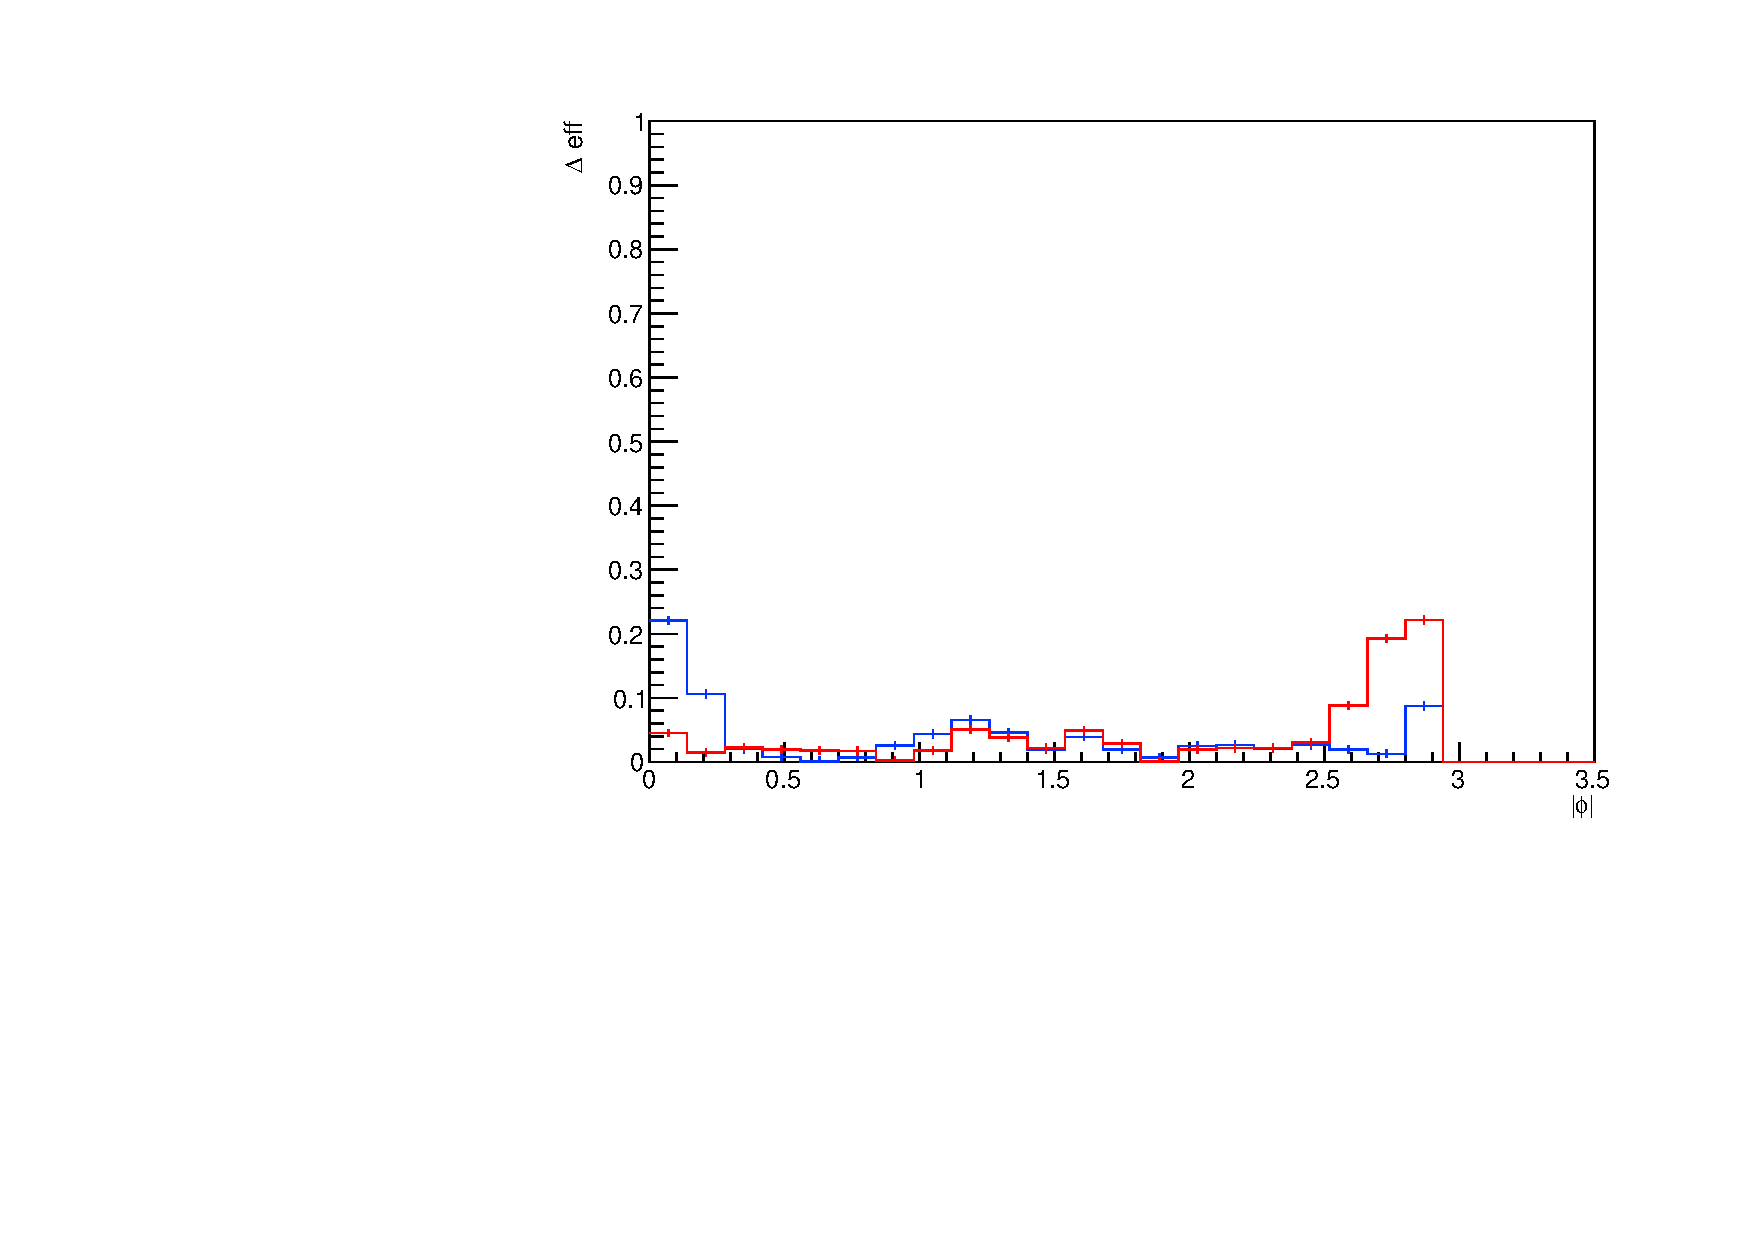
\includegraphics[width=0.9\textwidth]{first/up_pdf/test_u/h_phi_test_SPi_combined.pdf}
\end{subfigure}
\begin{subfigure}{0.45\textwidth}
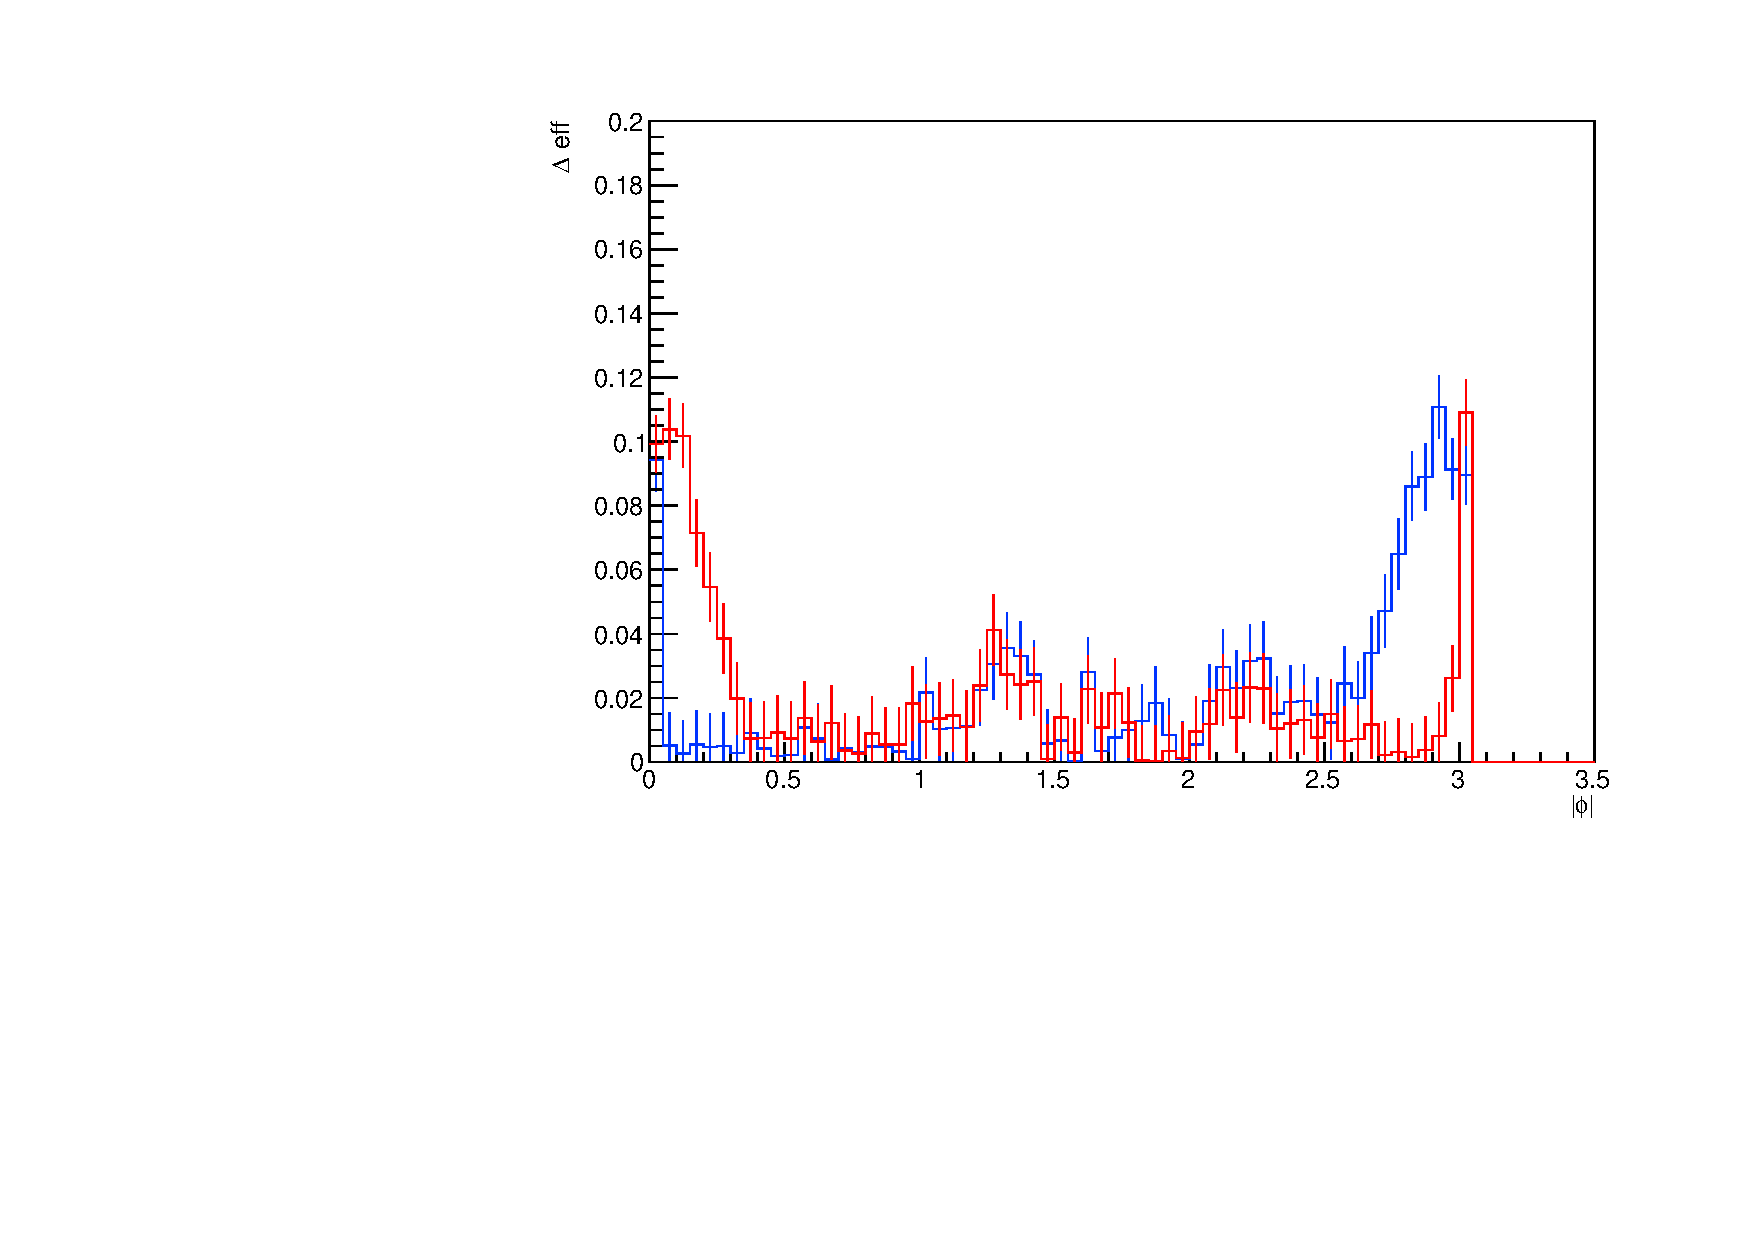
\includegraphics[width=0.9\textwidth]{first/down_pdf/test_d/h_phi_test_SPi_combined.pdf}
\end{subfigure}
\end{figure}
\end{frame}
\begin{frame}{Total Efficiencies - before cut}
\begin{table}
\resizebox{\textwidth}{!}{
	\begin{tabular}{cS[table-format=2.2]@{${}\pm{}$}S[table-format=1.2]S[table-format=2.2]@{${}\pm{}$}S[table-format=1.2]S[table-format=2.2]@{${}\pm{}$}S[table-format=1.2]S[table-format=2.2]@{${}\pm{}$}S[table-format=1.2]S[table-format=2.2]@{${}\pm{}$}S[table-format=1.2]}
		\toprule
		{Polarity} & \multicolumn{2}{c}{$\epsilon_{\pi} $} & \multicolumn{2}{c}{$\epsilon_{K} $} & \multicolumn{2}{c}{$ \epsilon_{\pi,s} $} & \multicolumn{2}{c}{$\epsilon_{D^0} $} & \multicolumn{2}{c}{$\epsilon_{D^*} $} \\
		\midrule
		$UP$ & 86.65 & 0.01 & 84.63 & 0.01 & 76.65 & 0.02 & 73.34 & 0.02 & 56.31 & 0.02\\
		$DOWN$ & 86.68 & 0.01 & 84.67 & 0.01 & 76.66 & 0.02 & 73.39 & 0.02 & 56.35 & 0.02\\
		\bottomrule
	\end{tabular}}
\end{table}
\end{frame}

\begin{frame}{Total Efficiencies - after cut}
\begin{table}
\resizebox{\textwidth}{!}{
	\begin{tabular}{cS[table-format=2.2]@{${}\pm{}$}S[table-format=1.2]S[table-format=2.2]@{${}\pm{}$}S[table-format=1.2]S[table-format=2.2]@{${}\pm{}$}S[table-format=1.2]S[table-format=2.2]@{${}\pm{}$}S[table-format=1.2]S[table-format=2.2]@{${}\pm{}$}S[table-format=1.2]}
		\toprule
		{Polarity} & \multicolumn{2}{c}{$\epsilon_{\pi} $} & \multicolumn{2}{c}{$\epsilon_{K} $} & \multicolumn{2}{c}{$ \epsilon_{\pi,s} $} & \multicolumn{2}{c}{$\epsilon_{D^0} $} & \multicolumn{2}{c}{$\epsilon_{D^*} $} \\
		\midrule
		$UP$ & 86.65 & 0.01 & 84.63 & 0.01 & 50.23 & 0.02 & 73.34 & 0.02 & 36.61 & 0.02\\
		$DOWN$ & 86.68 & 0.01 & 84.67 & 0.01 & 50.25 & 0.02 & 73.39 & 0.02 & 36.58 & 0.02\\
		\bottomrule
	\end{tabular}}
\end{table}
\end{frame}
\begin{frame}
\begin{LARGE}
\textbf{Charge: +}
\end{LARGE}
\end{frame}
\begin{frame}{Numbers - before cut}
\begin{table}
\resizebox{\textwidth}{!}{
%	\caption{UP Polarity - reconstructed vs. total number of events}
	\begin{tabular}{cS[table-format=6.0]S[table-format=6.0]S[table-format=6.0]S[table-format=6.0]S[table-format=6.0]}
		\toprule
		{UP} & {$\pi $} & {$K $} & {$ soft\, \pi $} & {$D^0 $} & {$D^* $} \\
		\midrule
		$N_\text{reco}$ & 2669990 & 2620280 & 2352910 & 2249370 & 1720940 \\
		$N_\text{tot}$ & 3000000 & 3000000 & 3000000 & 3000000 & 3000000 \\
		\bottomrule
	\end{tabular}}
\resizebox{\textwidth}{!}{
%	\caption{DOWN Polarity - reconstructed vs. total number of events}
	\begin{tabular}{cS[table-format=6.0]S[table-format=6.0]S[table-format=6.0]S[table-format=6.0]S[table-format=6.0]}
		\toprule
		{DOWN} & {$\pi $} & {$K $} & {$ soft\, \pi $} & {$D^0 $} & {$D^* $} \\
		\midrule
		$N_\text{reco}$ & 2674000 & 2626350 & 2374360 & 2253370 & 1737460 \\
		$N_\text{tot}$ & 3000000 & 3000000 & 3000000 & 3000000 & 3000000 \\
		\bottomrule
	\end{tabular}}
\end{table}
\end{frame}
\begin{frame}{Numbers - after cut}
\begin{table}
\resizebox{\textwidth}{!}{
%	\caption{UP Polarity - reconstructed vs. total number of events}
	\begin{tabular}{cS[table-format=6.0]S[table-format=6.0]S[table-format=6.0]S[table-format=6.0]S[table-format=6.0]}
		\toprule
		{UP} & {$\pi $} & {$K $} & {$ soft\, \pi $} & {$D^0 $} & {$D^* $} \\
		\midrule
		$N_\text{reco}$ & 2669990 & 2620280 & 1546670 & 2249370 & 1121530 \\
		$N_\text{tot}$ & 3000000 & 3000000 & 1961330 & 3000000 & 1961330 \\
		%$N_\text{reco}$ & 2669990 & 2620280 & 1706180 & 2249370 & 1241100 \\
		%$N_\text{tot}$ & 3000000 & 3000000 & 2157840 & 3000000 & 2157840 \\
		\bottomrule
	\end{tabular}}
\resizebox{\textwidth}{!}{
%	\caption{DOWN Polarity - reconstructed vs. total number of events}
	\begin{tabular}{cS[table-format=6.0]S[table-format=6.0]S[table-format=6.0]S[table-format=6.0]S[table-format=6.0]}
		\toprule
		{DOWN} & {$\pi $} & {$K $} & {$ soft\, \pi $} & {$D^0 $} & {$D^* $} \\
		\midrule
		$N_\text{reco}$ & 2674000 & 2626350 & 1552010 & 2253370 & 1125280 \\
		$N_\text{tot}$ & 3000000 & 3000000 & 1963510 & 3000000 & 1963510 \\
		%$N_\text{reco}$ & 2674000 & 2626350 & 1697140 & 2253370 & 1234900 \\
		%$N_\text{tot}$ & 3000000 & 3000000 & 2159820 & 3000000 & 2159820 \\
		\bottomrule
	\end{tabular}}
\end{table}
\end{frame}
\begin{frame}
\begin{LARGE}
\textbf{Charge: -}
\end{LARGE}
\end{frame}
\begin{frame}{Numbers - before cut}
\begin{table}
\resizebox{\textwidth}{!}{
%	\caption{UP Polarity - reconstructed vs. total number of events}
	\begin{tabular}{cS[table-format=6.0]S[table-format=6.0]S[table-format=6.0]S[table-format=6.0]S[table-format=6.0]}
		\toprule
		{UP} & {$\pi $} & {$K $} & {$ soft\, \pi $} & {$D^0 $} & {$D^* $} \\
		\midrule
		$N_\text{reco}$ & 2669990 & 2620280 & 2352910 & 2249370 & 1720940 \\
		$N_\text{tot}$ & 3000000 & 3000000 & 3000000 & 3000000 & 3000000 \\
		\bottomrule
	\end{tabular}}
\resizebox{\textwidth}{!}{
%	\caption{DOWN Polarity - reconstructed vs. total number of events}
	\begin{tabular}{cS[table-format=6.0]S[table-format=6.0]S[table-format=6.0]S[table-format=6.0]S[table-format=6.0]}
		\toprule
		{DOWN} & {$\pi $} & {$K $} & {$ soft\, \pi $} & {$D^0 $} & {$D^* $} \\
		\midrule
		$N_\text{reco}$ & 2674000 & 2626350 & 2374360 & 2253370 & 1737460 \\
		$N_\text{tot}$ & 3000000 & 3000000 & 3000000 & 3000000 & 3000000 \\
		\bottomrule
	\end{tabular}}
\end{table}
\end{frame}
\begin{frame}{Numbers - after cut}
\begin{table}
\resizebox{\textwidth}{!}{
%	\caption{UP Polarity - reconstructed vs. total number of events}
	\begin{tabular}{cS[table-format=6.0]S[table-format=6.0]S[table-format=6.0]S[table-format=6.0]S[table-format=6.0]}
		\toprule
		{UP} & {$\pi $} & {$K $} & {$ soft\, \pi $} & {$D^0 $} & {$D^* $} \\
		\midrule
		$N_\text{reco}$ & 2669990 & 2620280 & 1549090 & 2249370 & 1132970 \\
		$N_\text{tot}$ & 3000000 & 3000000 & 1960630 & 3000000 & 1960630 \\
		\bottomrule
	\end{tabular}}
\resizebox{\textwidth}{!}{
%	\caption{DOWN Polarity - reconstructed vs. total number of events}
	\begin{tabular}{cS[table-format=6.0]S[table-format=6.0]S[table-format=6.0]S[table-format=6.0]S[table-format=6.0]}
		\toprule
		{DOWN} & {$\pi $} & {$K $} & {$ soft\, \pi $} & {$D^0 $} & {$D^* $} \\
		\midrule
		$N_\text{reco}$ & 2674000 & 2626350 & 1549160 & 2253370 & 1134370 \\
		$N_\text{tot}$ & 3000000 & 3000000 & 1964560 & 3000000 & 1964560 \\
		\bottomrule
	\end{tabular}}
\end{table}
\end{frame}
\begin{frame}{Deviation before \& after cut}
\begin{table}
	\caption{The deviation $\frac{N_+ - N_-}{N_+ + N_-}/10^{-3}$}
	\resizebox{\textwidth}{!}{
	\begin{tabular}{cS[table-format=1.1]@{${}\pm{}$}S[table-format=1.1]S[table-format=1.1]@{${}\pm{}$}S[table-format=1.1]S[table-format=1.1]@{${}\pm{}$}S[table-format=1.1]S[table-format=1.1]@{${}\pm{}$}S[table-format=1.1]S[table-format=1.1]@{${}\pm{}$}S[table-format=1.1]}
		\toprule
		{Polarity} & \multicolumn{2}{c}{$\pi $} & \multicolumn{2}{c}{$ K $} & \multicolumn{2}{c}{$ soft \pi $} & \multicolumn{2}{c}{$ D^0 $} & \multicolumn{2}{c}{$ D^* $} \\
		\midrule
		$UP$ & -0.1 & 0.4 & 4.7 & 0.4 & -3.8 & 0.5 & -4.7 & 0.5 & -8.2 & 0.5 \\
		$DOWN$ & -0.3 & 0.4 & 5.2 & 0.4 & 3.7 & 0.5 & -5.0 & 0.5 & -0.8 & 0.5\\
		\bottomrule
	\end{tabular}}
	\resizebox{\textwidth}{!}{
	\begin{tabular}{cS[table-format=1.1]@{${}\pm{}$}S[table-format=1.1]S[table-format=1.1]@{${}\pm{}$}S[table-format=1.1]S[table-format=1.1]@{${}\pm{}$}S[table-format=1.1]S[table-format=1.1]@{${}\pm{}$}S[table-format=1.1]S[table-format=1.1]@{${}\pm{}$}S[table-format=1.1]}
		\toprule
		{Polarity} & \multicolumn{2}{c}{$\pi $} & \multicolumn{2}{c}{$ K $} & \multicolumn{2}{c}{$ soft \pi $} & \multicolumn{2}{c}{$ D^0 $} & \multicolumn{2}{c}{$ D^* $} \\
		\midrule
		$UP$ & -0.1 & 0.4 & 4.7 & 0.4 & -0.8 & 0.6 & -4.7 & 0.5 & -5.1 & 0.7\\
		$DOWN$ & -0.3 & 0.4 & 5.2 & 0.4 & 0.9 & 0.5 & -5.0 & 0.5 & -4.0 & 0.7\\
		\bottomrule
	\end{tabular}}
\end{table}
\begin{itemize}
\item deviation in $\pi$ gets smaller, in $D^*$ equals out
\item $\approx 33\%$ of events is rejected
\end{itemize}
\end{frame}
\begin{frame}{Comparison of different charges with $UP$ polarity - soft $\pi$}
\begin{figure}
\begin{subfigure}{0.45\textwidth}
\includegraphics[width=0.9\textwidth]{first/up_pdf/combined/h_pt_reco_SPi.pdf}
\end{subfigure}
\begin{subfigure}{0.45\textwidth}
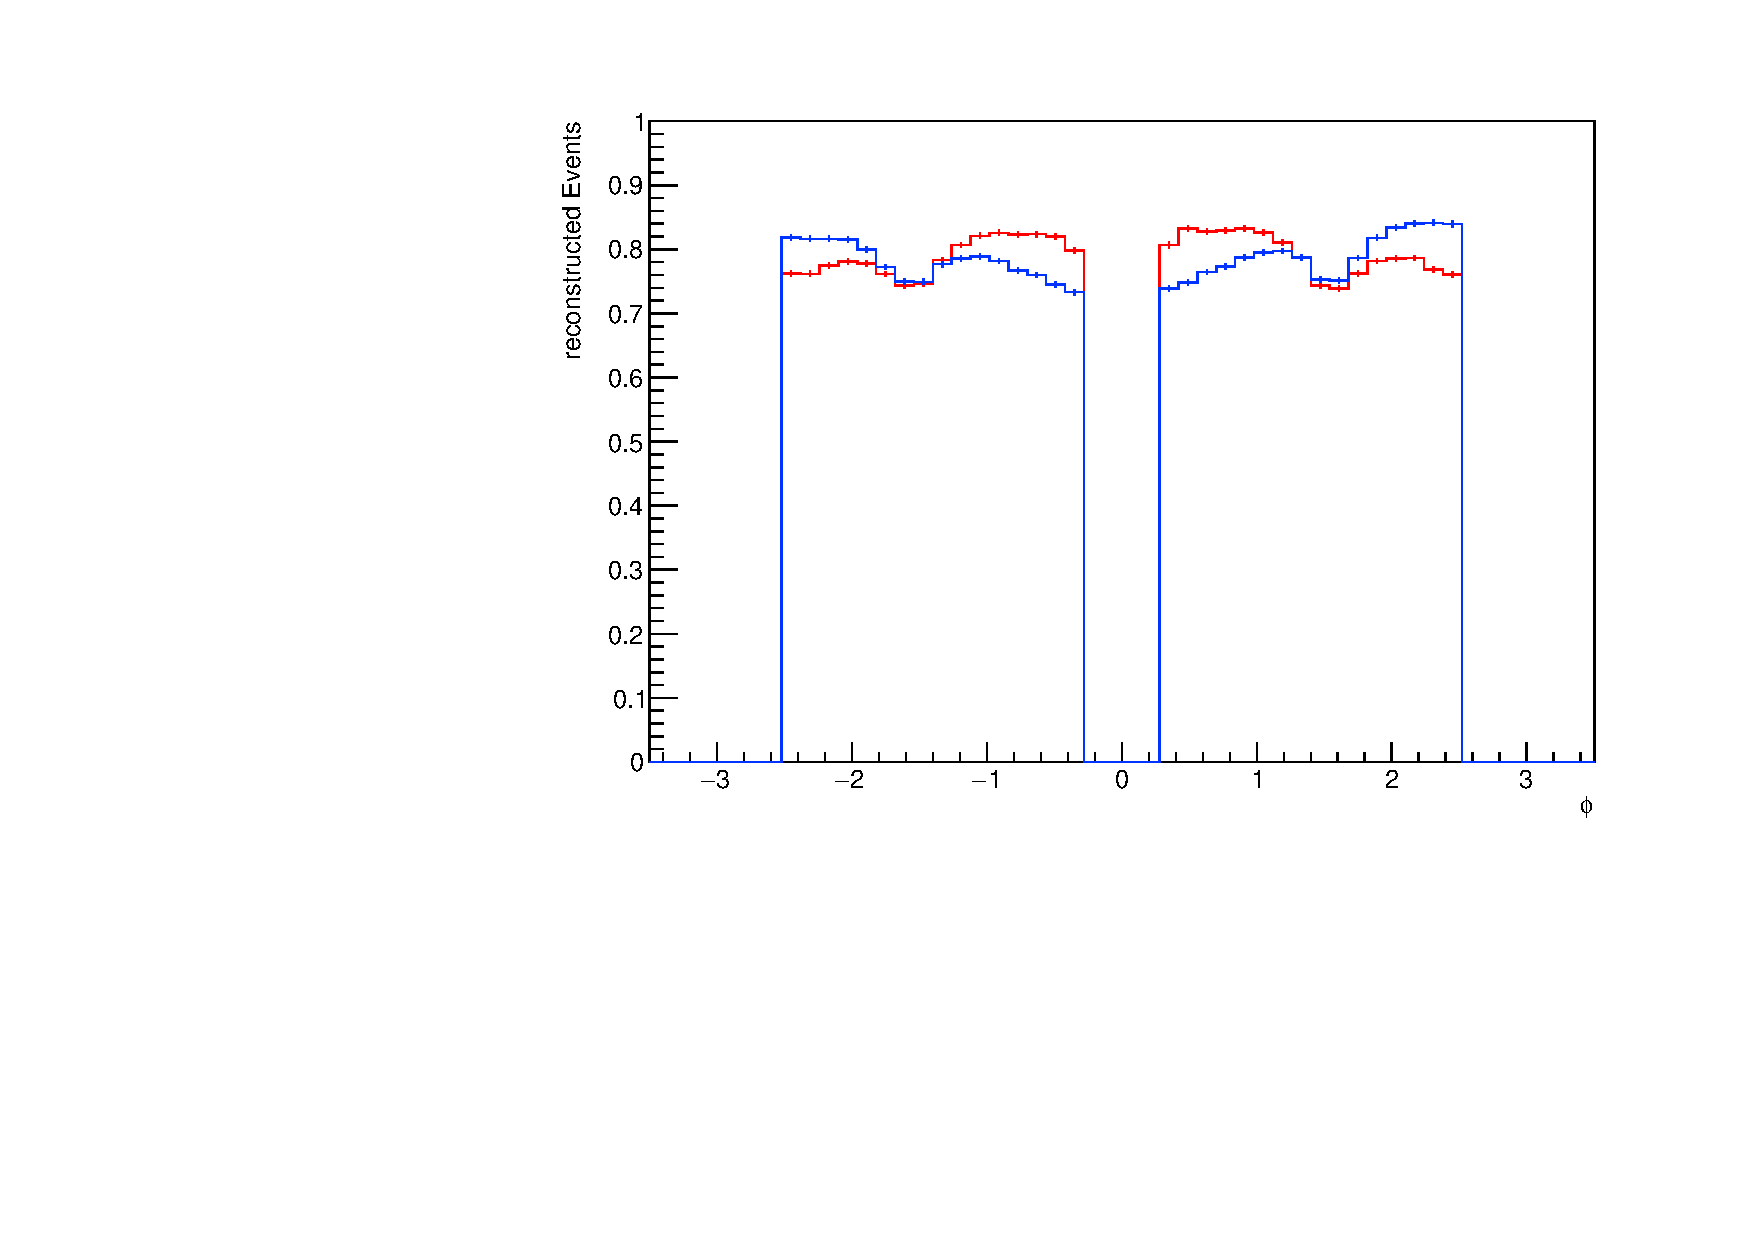
\includegraphics[width=0.9\textwidth]{first/up_pdf/combined/h_phi_reco_SPi.pdf}
\end{subfigure}
\begin{subfigure}{0.45\textwidth}
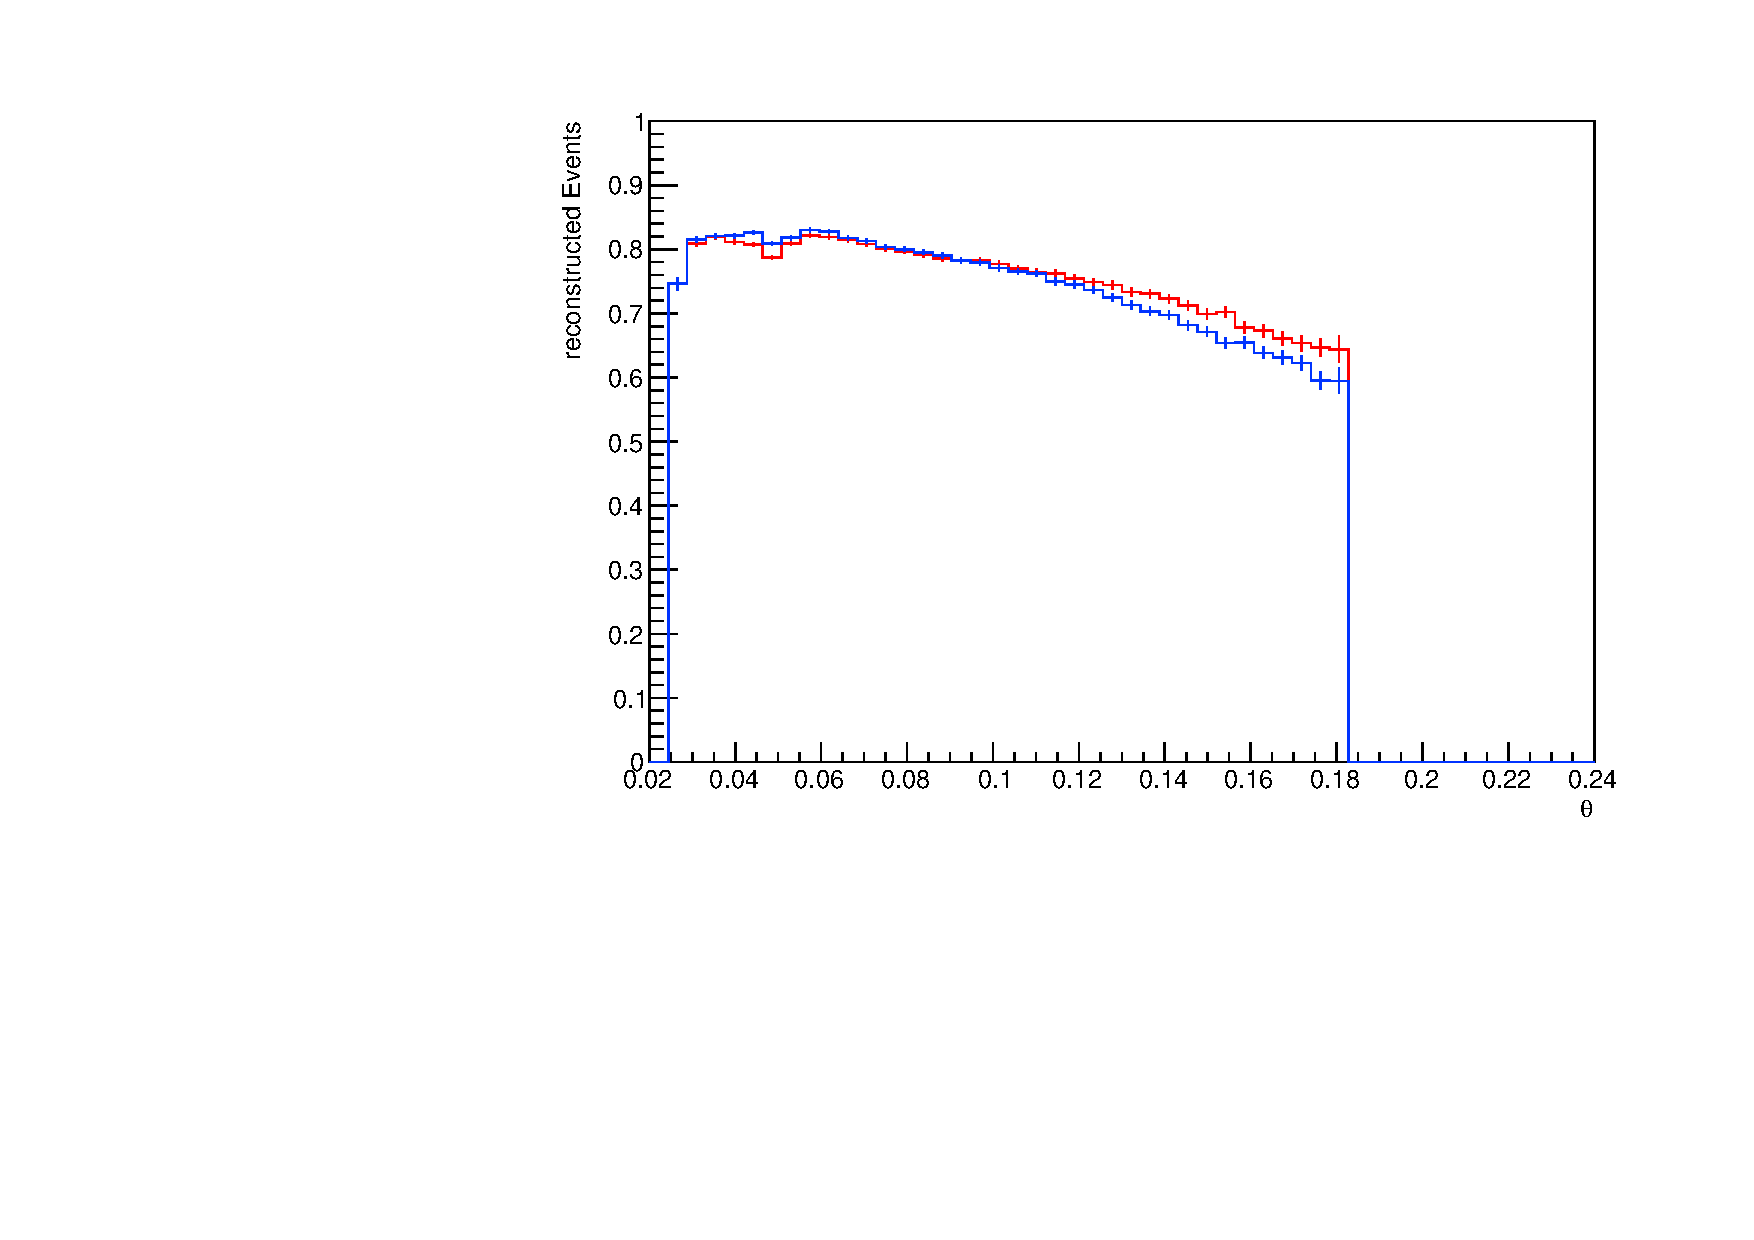
\includegraphics[width=0.9\textwidth]{first/up_pdf/combined/h_theta_reco_SPi.pdf}
\end{subfigure}
\begin{subfigure}{0.45\textwidth}
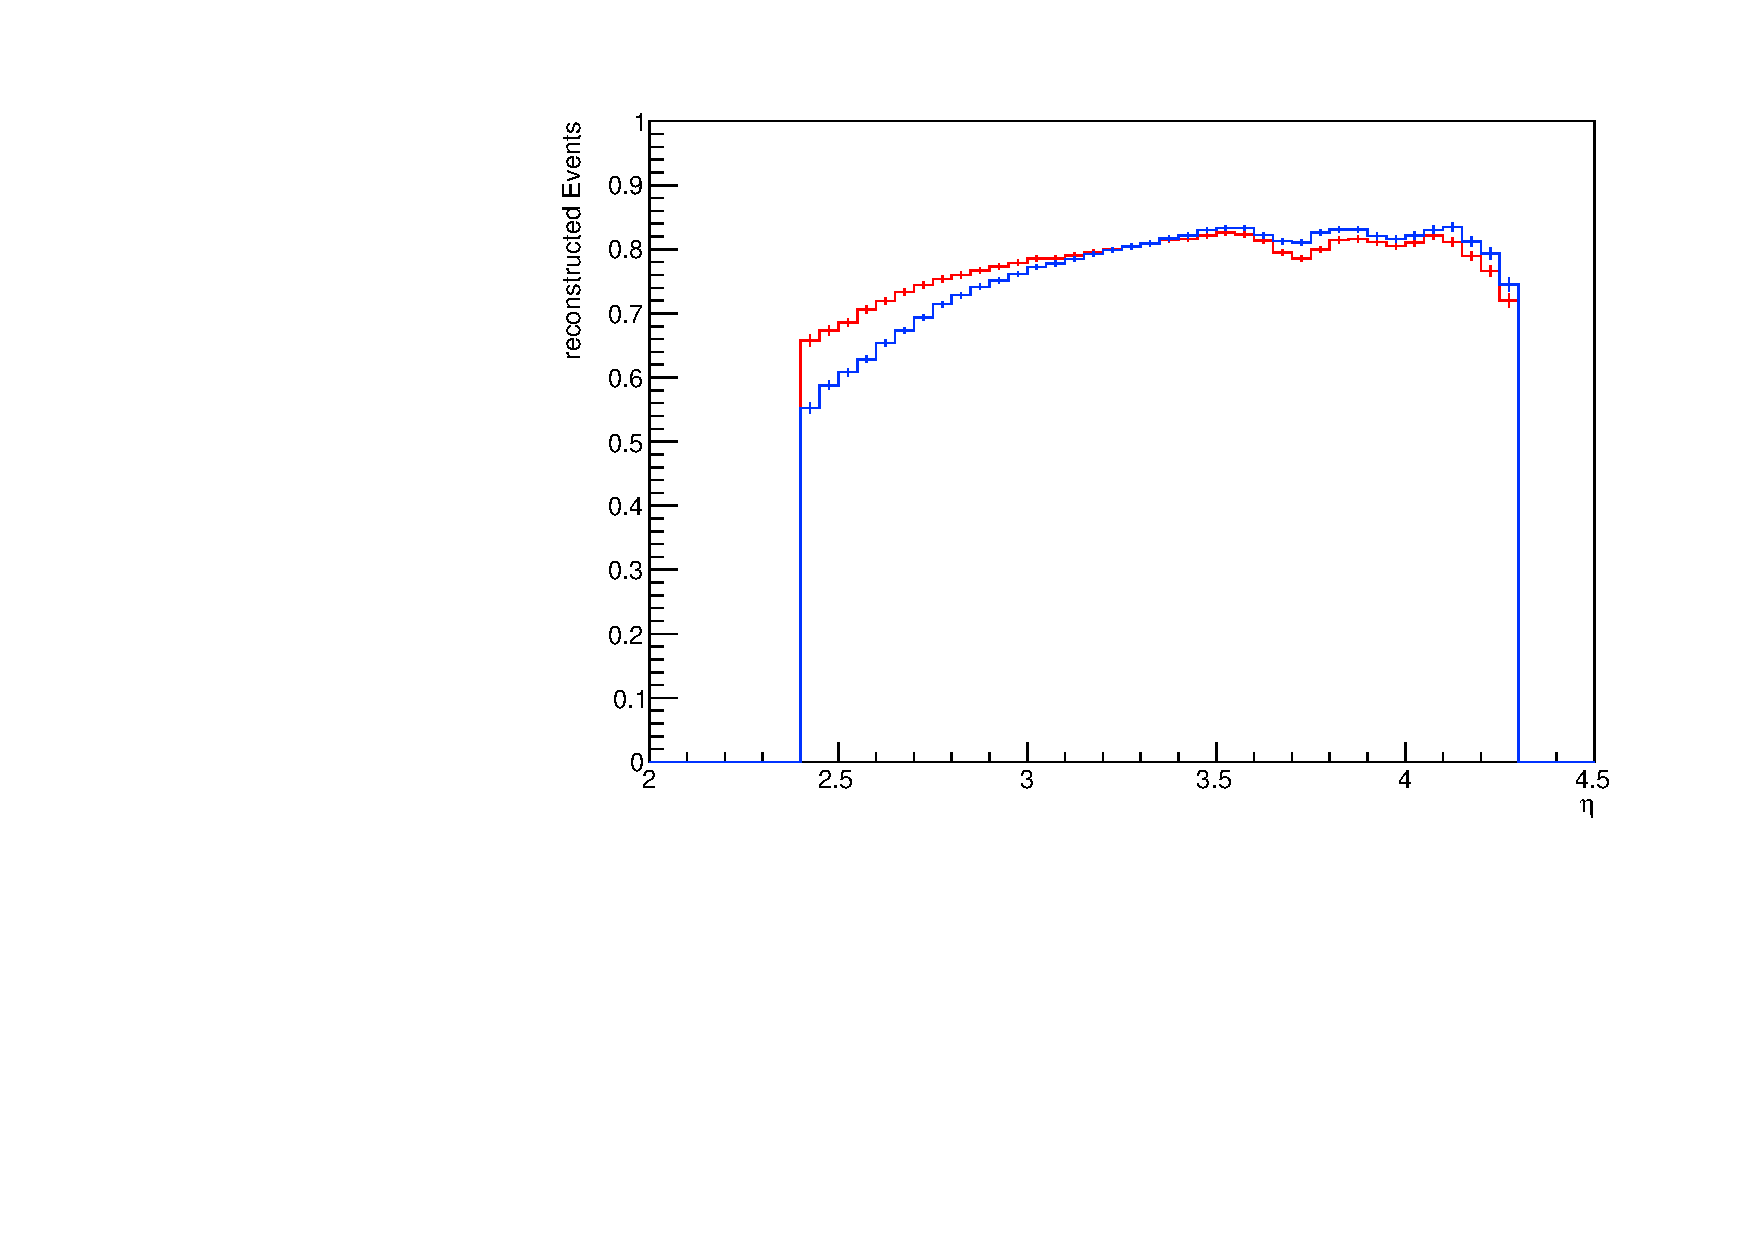
\includegraphics[width=0.9\textwidth]{first/up_pdf/combined/h_eta_reco_SPi.pdf}
\end{subfigure}
\end{figure}
\end{frame}
\begin{frame}{Comparison of different charges with $DOWN$ polarity - soft $\pi$}
\begin{figure}
\begin{subfigure}{0.45\textwidth}
\includegraphics[width=0.9\textwidth]{first/down_pdf/combined/h_pt_reco_SPi.pdf}
\end{subfigure}
\begin{subfigure}{0.45\textwidth}
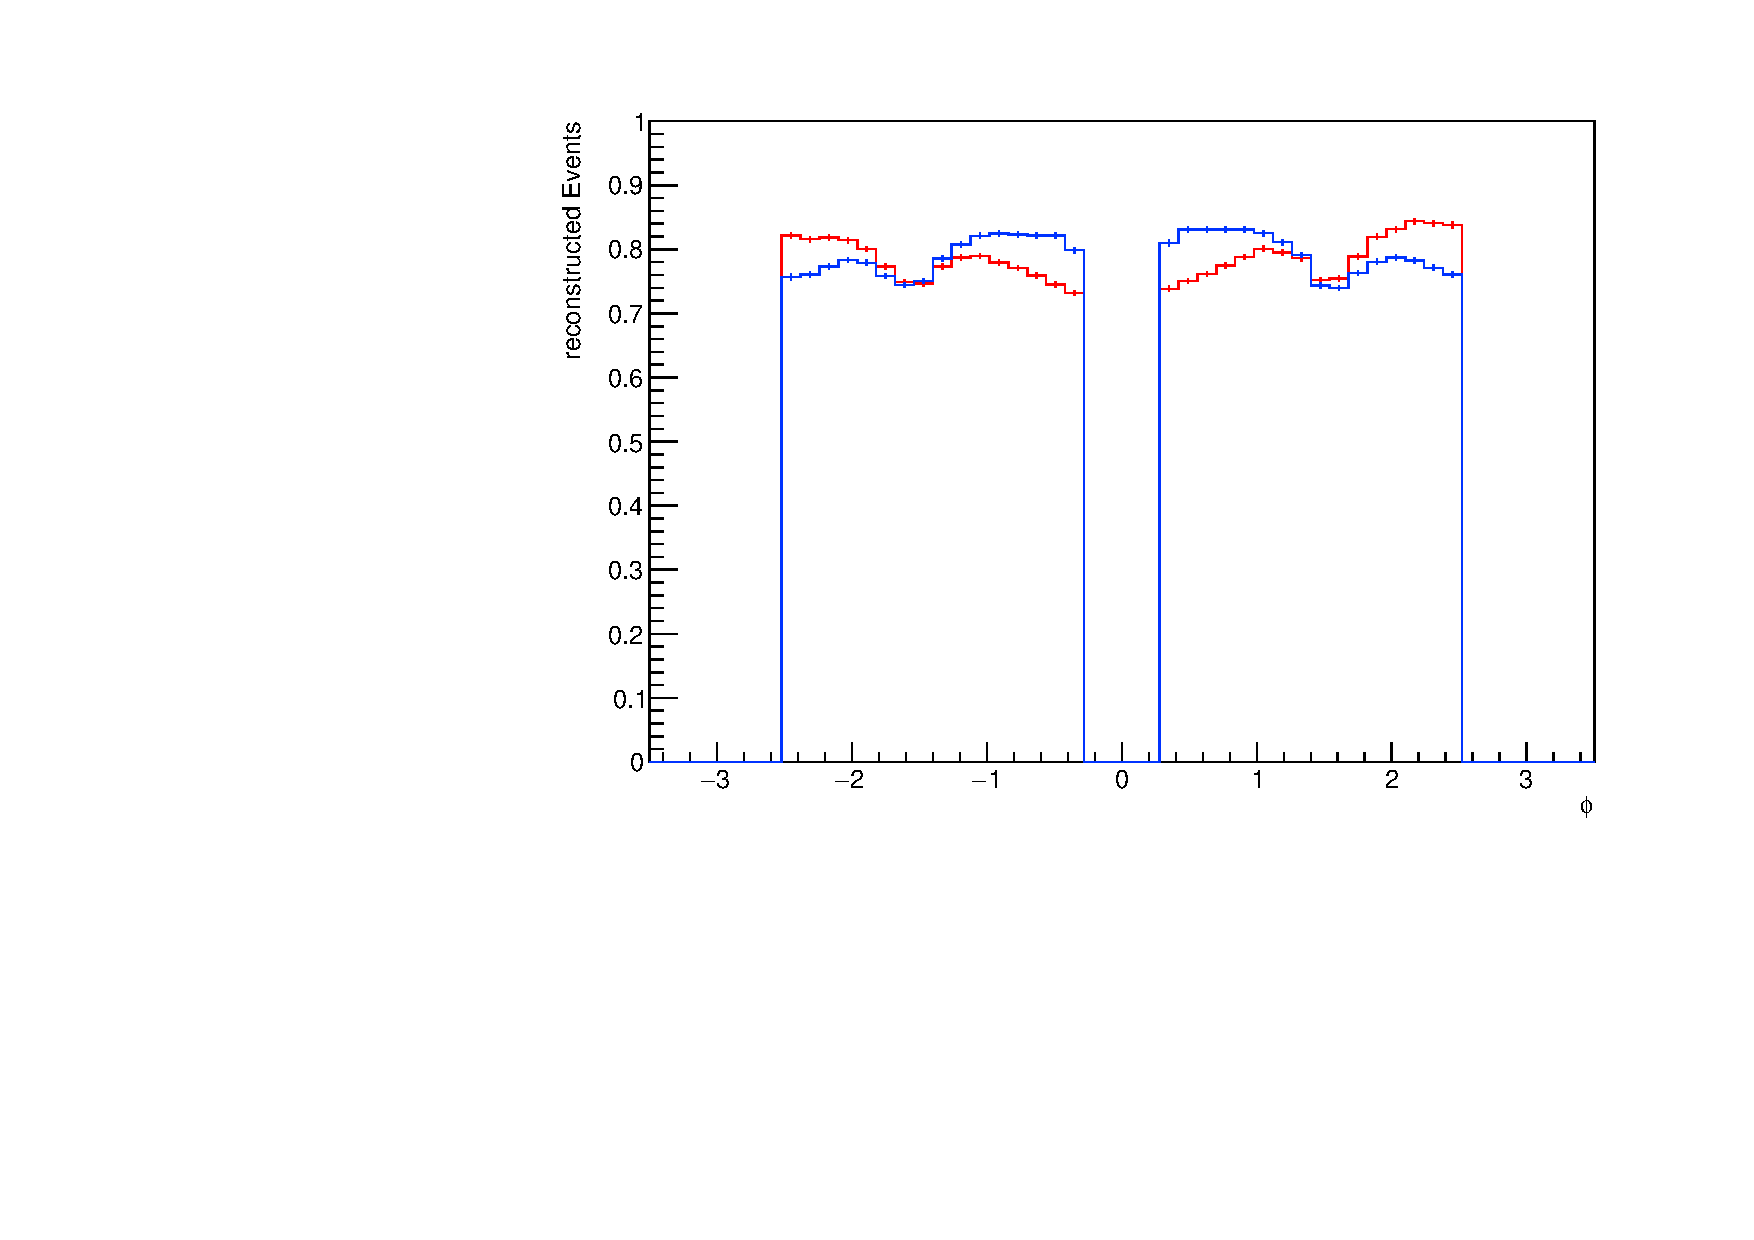
\includegraphics[width=0.9\textwidth]{first/down_pdf/combined/h_phi_reco_SPi.pdf}
\end{subfigure}
\begin{subfigure}{0.45\textwidth}
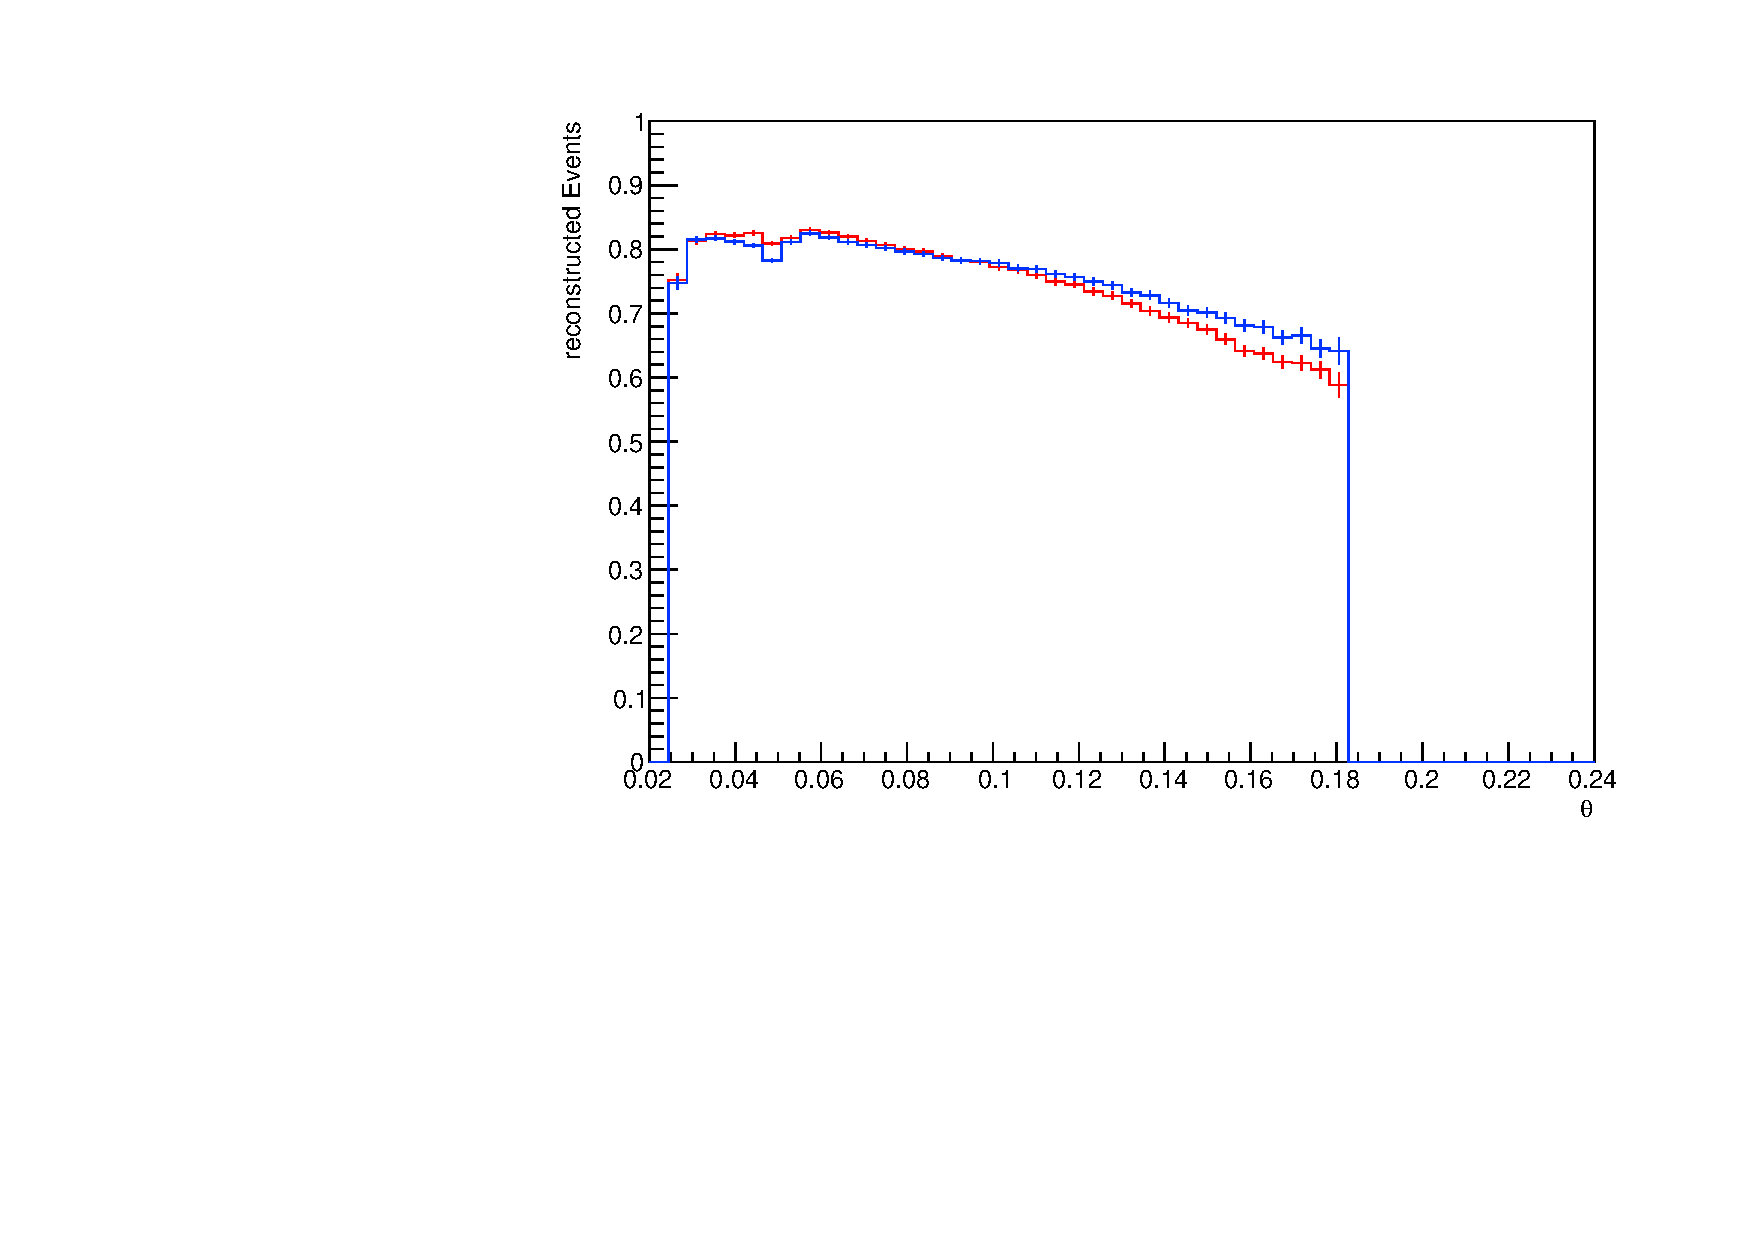
\includegraphics[width=0.9\textwidth]{first/down_pdf/combined/h_theta_reco_SPi.pdf}
\end{subfigure}
\begin{subfigure}{0.45\textwidth}
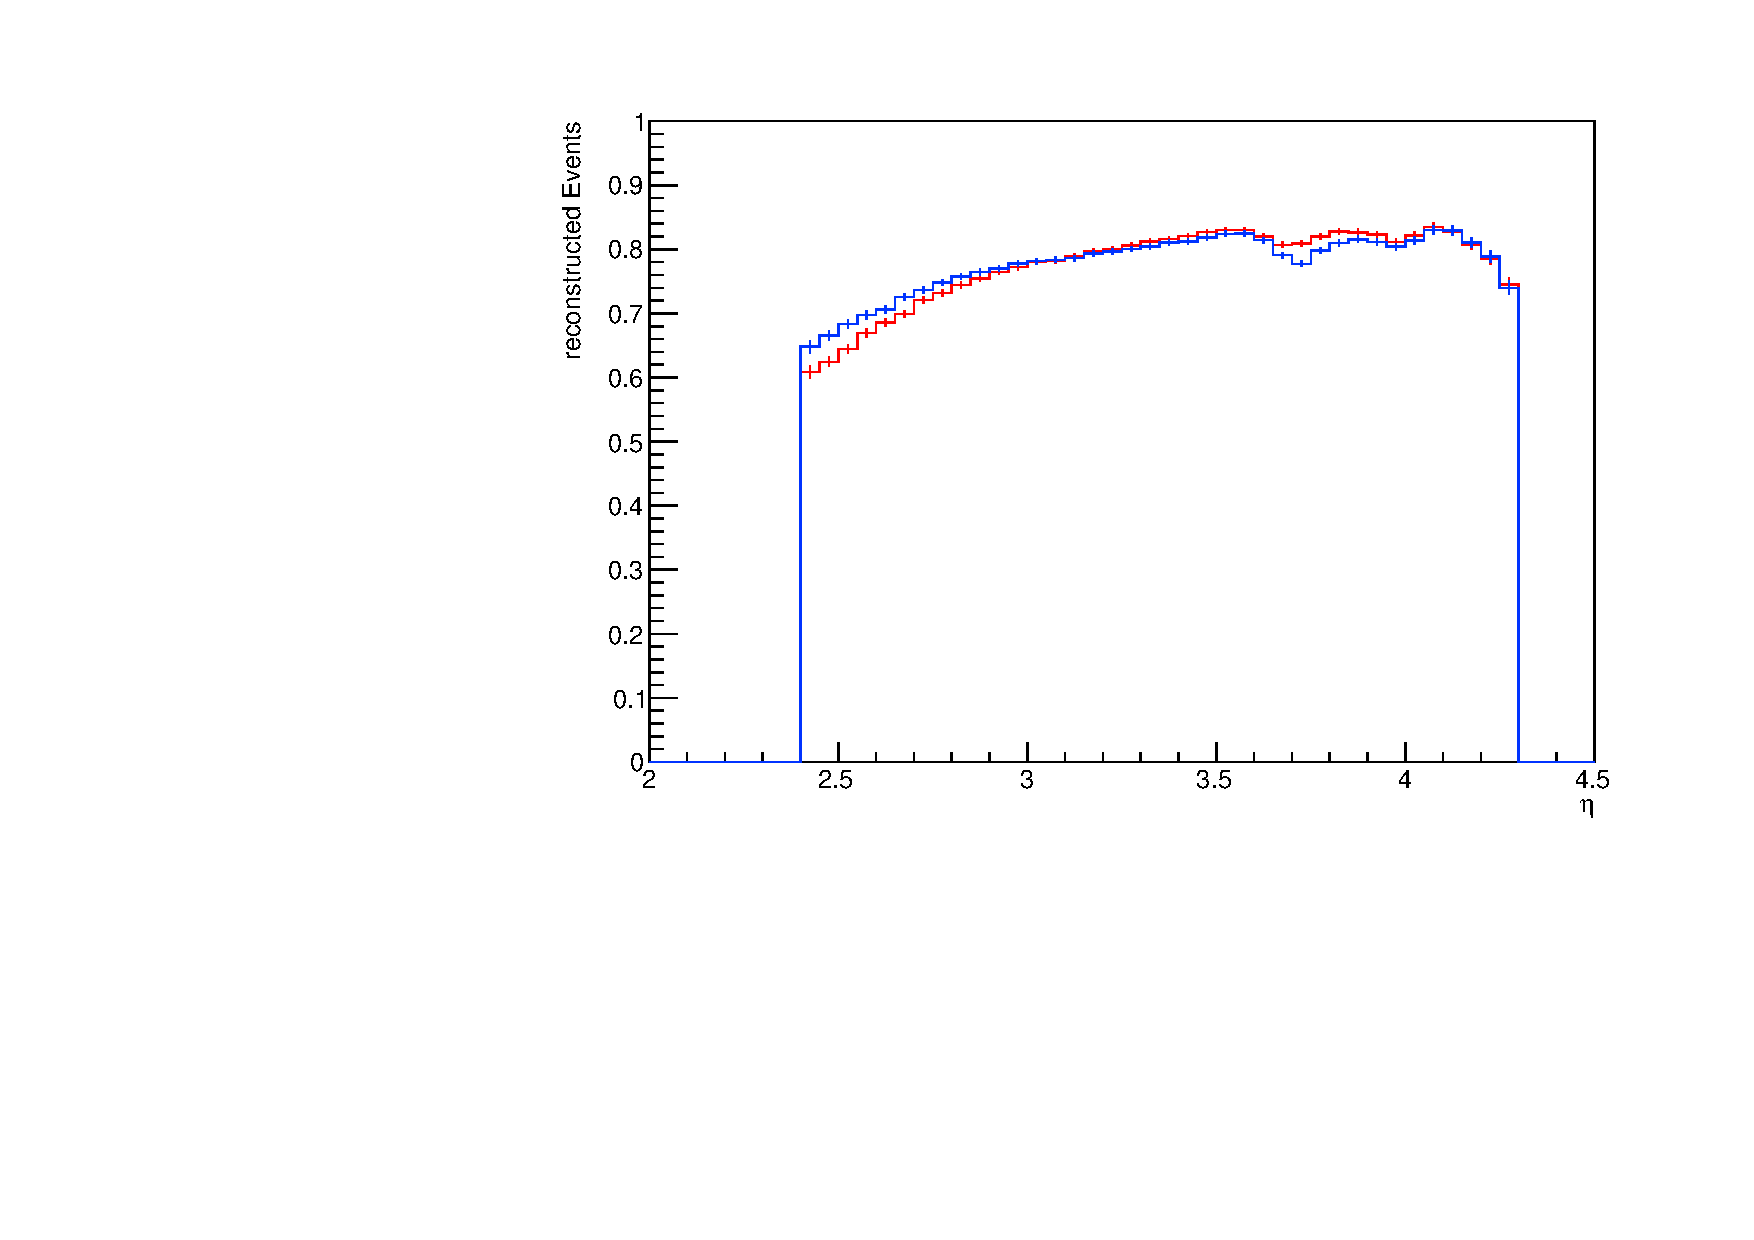
\includegraphics[width=0.9\textwidth]{first/down_pdf/combined/h_eta_reco_SPi.pdf}
\end{subfigure}
\end{figure}
\end{frame}
\begin{frame}{Comparison - soft $\pi p_\text{T}$}
\centering
\includegraphics[width=0.48\textwidth]{first/up_pdf/combined/h_pt_reco_SPi.pdf}
\includegraphics[width=0.48\textwidth]{first/down_pdf/combined/h_pt_reco_SPi.pdf}
\end{frame}
\begin{frame}{Comparison - soft $\pi \phi$}
\centering
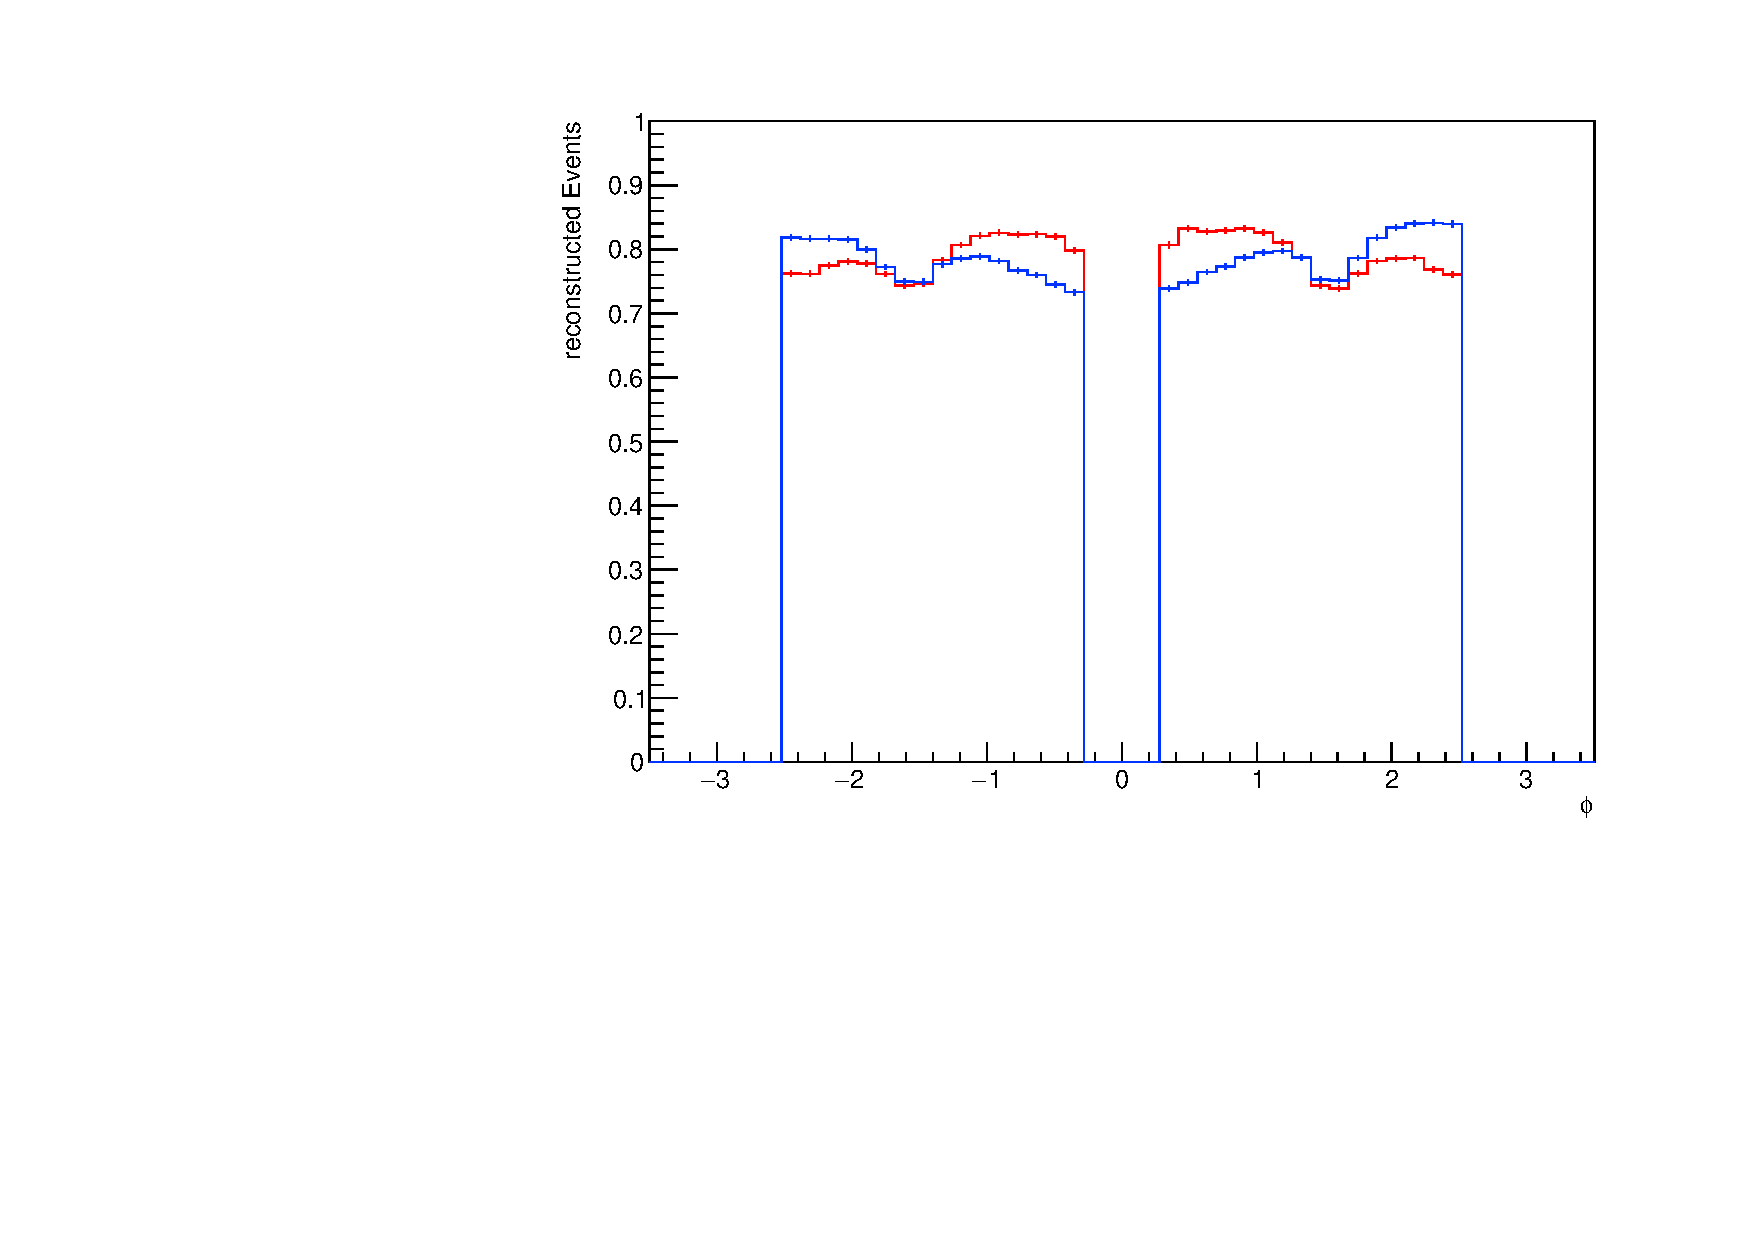
\includegraphics[width=0.48\textwidth]{first/up_pdf/combined/h_phi_reco_SPi.pdf}
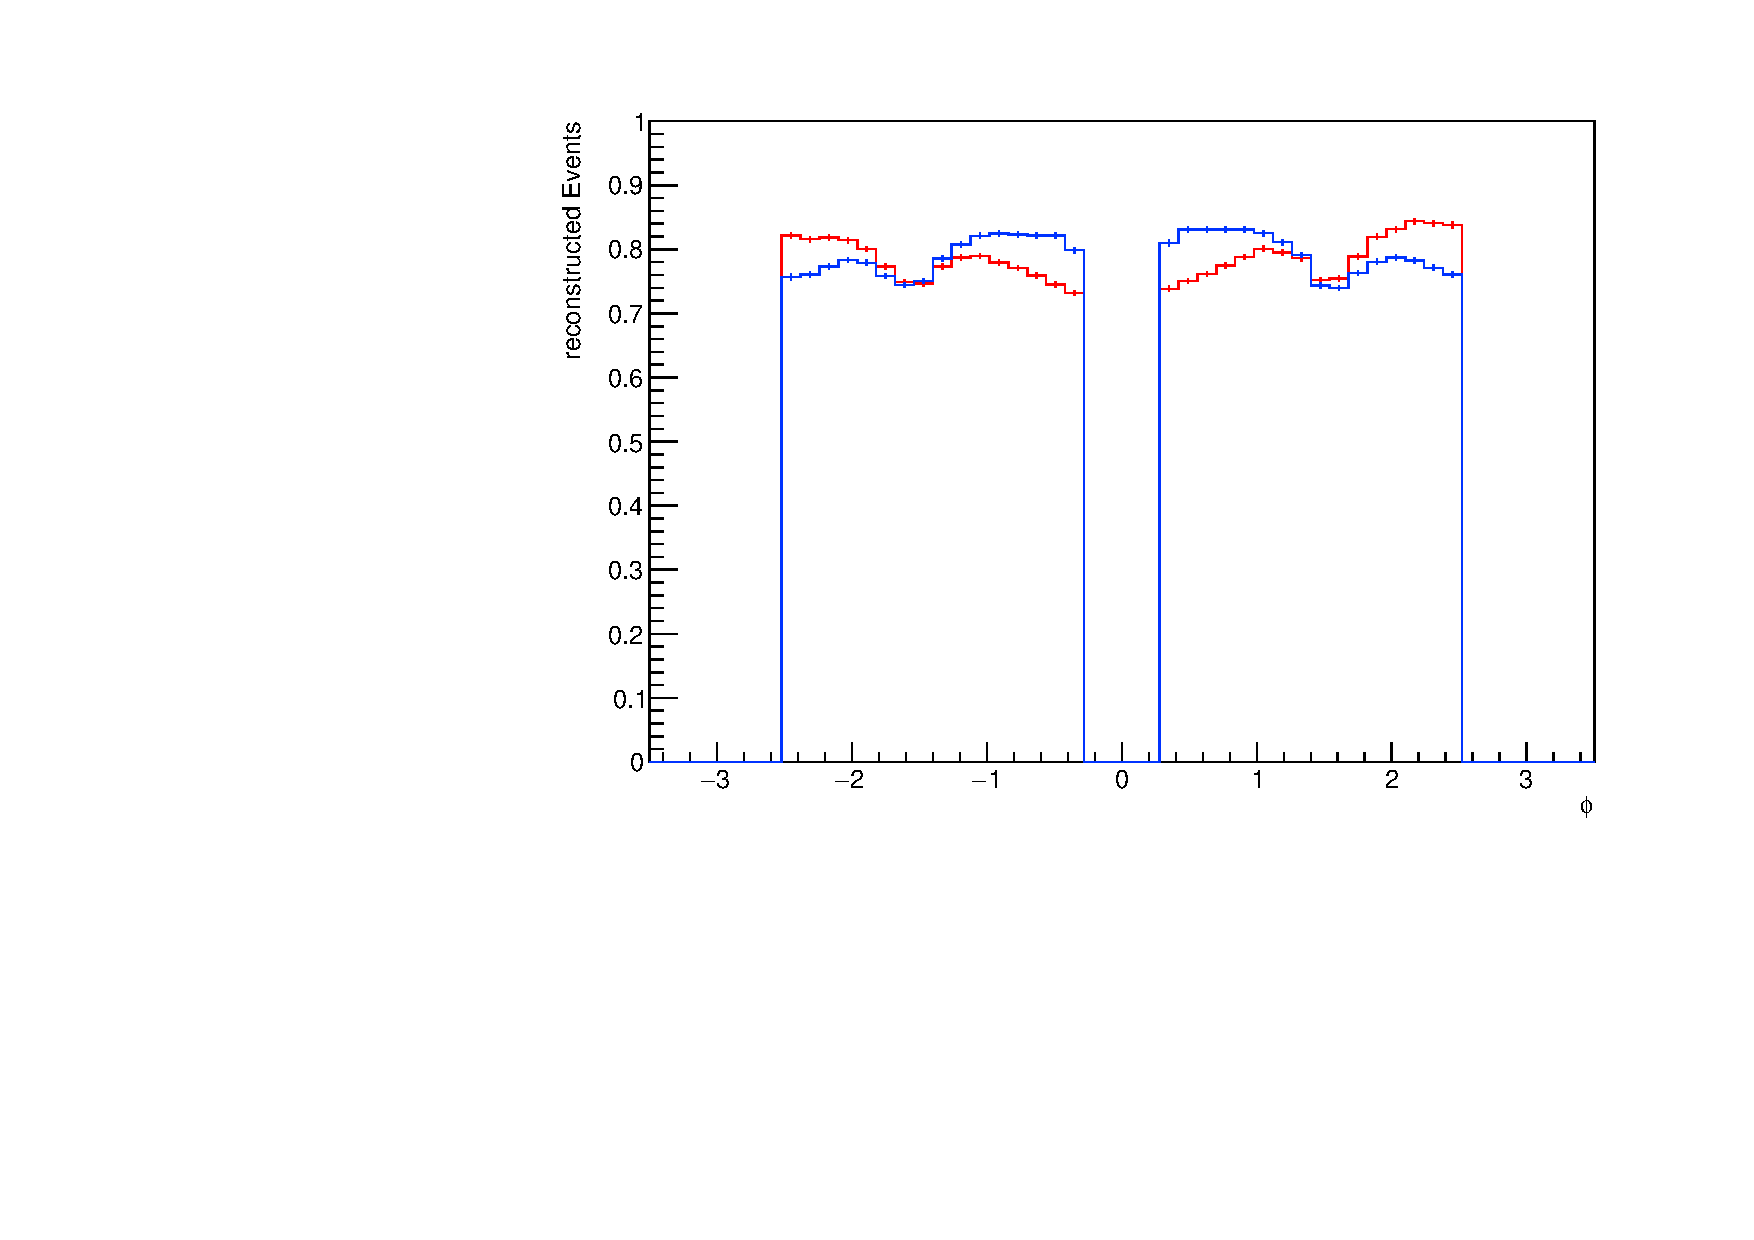
\includegraphics[width=0.48\textwidth]{first/down_pdf/combined/h_phi_reco_SPi.pdf}
\end{frame}
\begin{frame}{Comparison - soft $\pi \theta$}
\centering
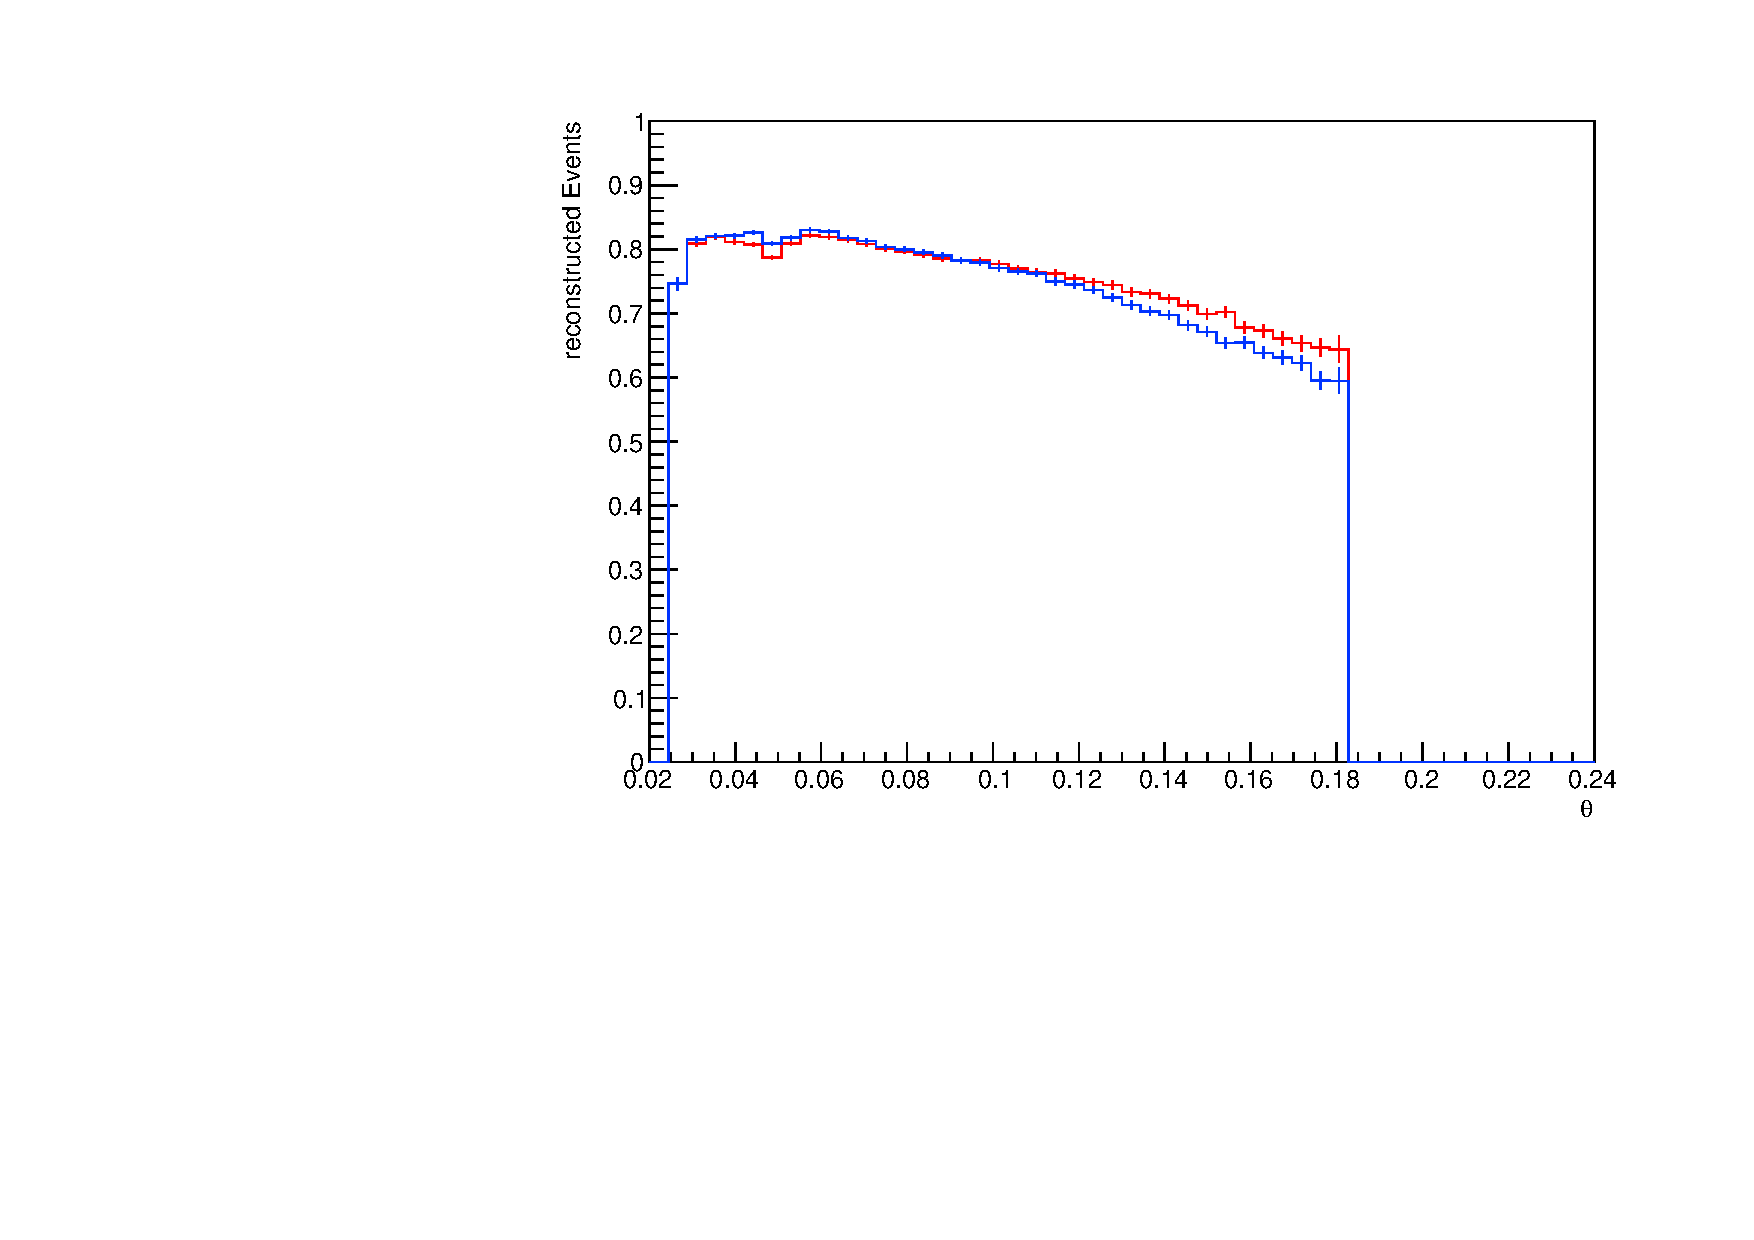
\includegraphics[width=0.48\textwidth]{first/up_pdf/combined/h_theta_reco_SPi.pdf}
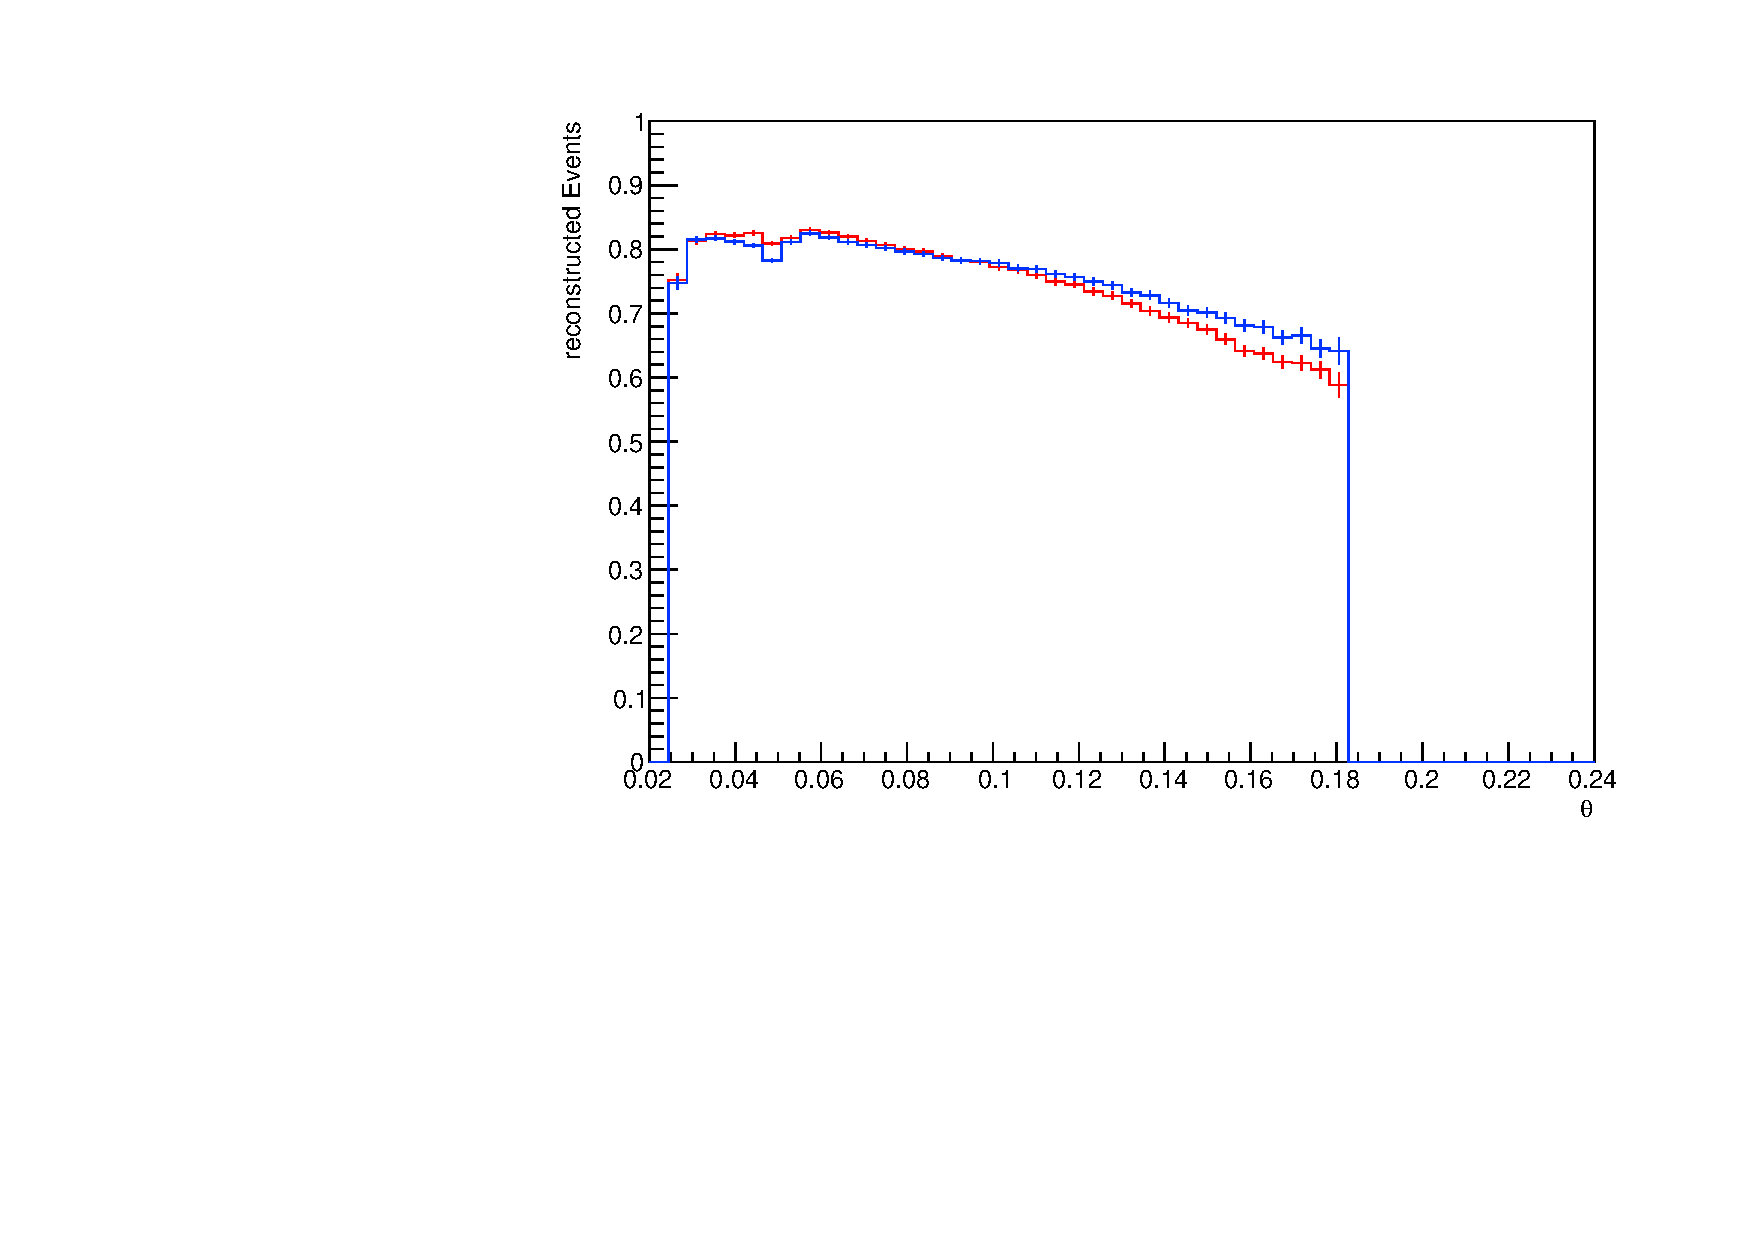
\includegraphics[width=0.48\textwidth]{first/down_pdf/combined/h_theta_reco_SPi.pdf}
\end{frame}
\begin{frame}{Comparison - soft $\pi \eta$}
\centering
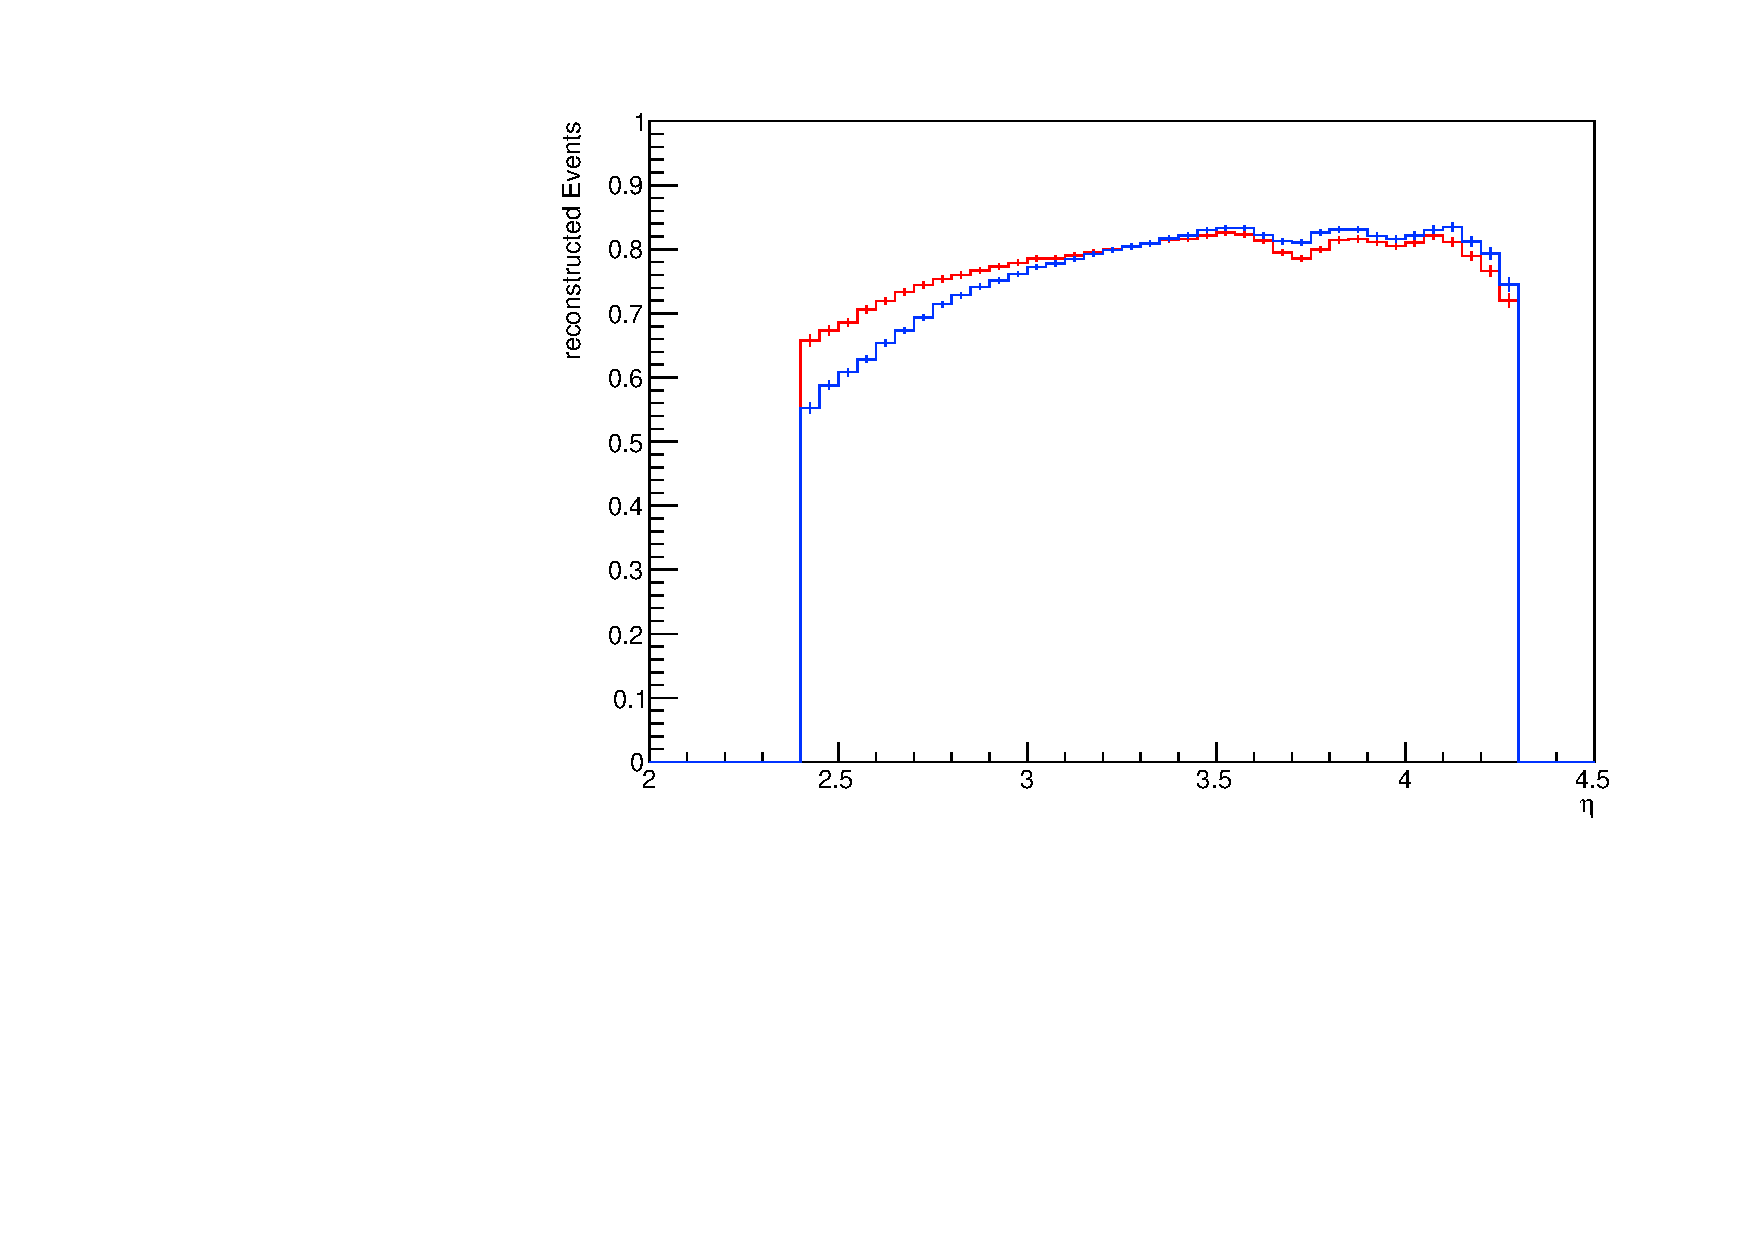
\includegraphics[width=0.48\textwidth]{first/up_pdf/combined/h_eta_reco_SPi.pdf}
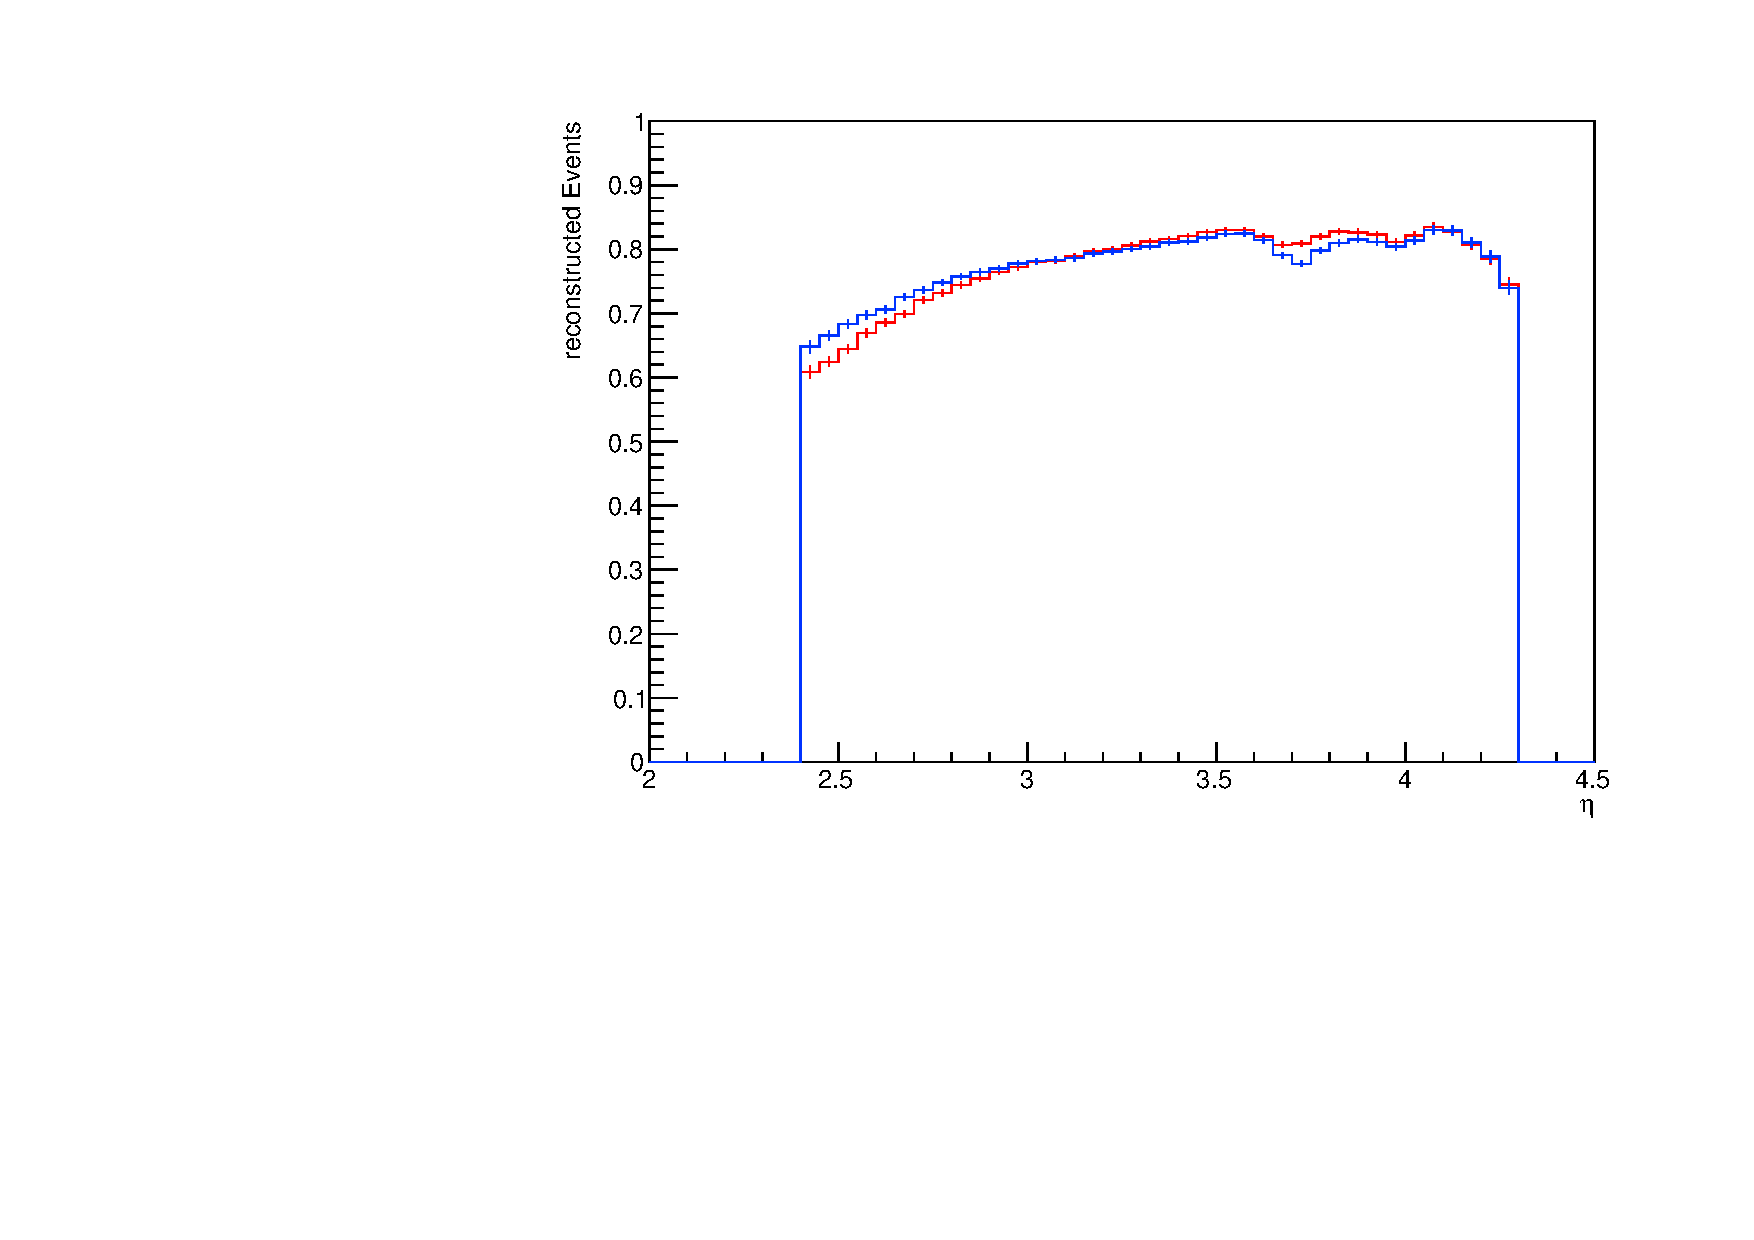
\includegraphics[width=0.48\textwidth]{first/down_pdf/combined/h_eta_reco_SPi.pdf}
\end{frame}
\begin{frame}{soft $\pi$ deviation dependencies - $UP$ polarity}
\begin{figure}
\begin{subfigure}{0.45\textwidth}
\includegraphics[width=0.9\textwidth]{first/up_pdf/deviation/h_pt_reco_SPi_pos_dev.pdf}
\end{subfigure}
\begin{subfigure}{0.45\textwidth}
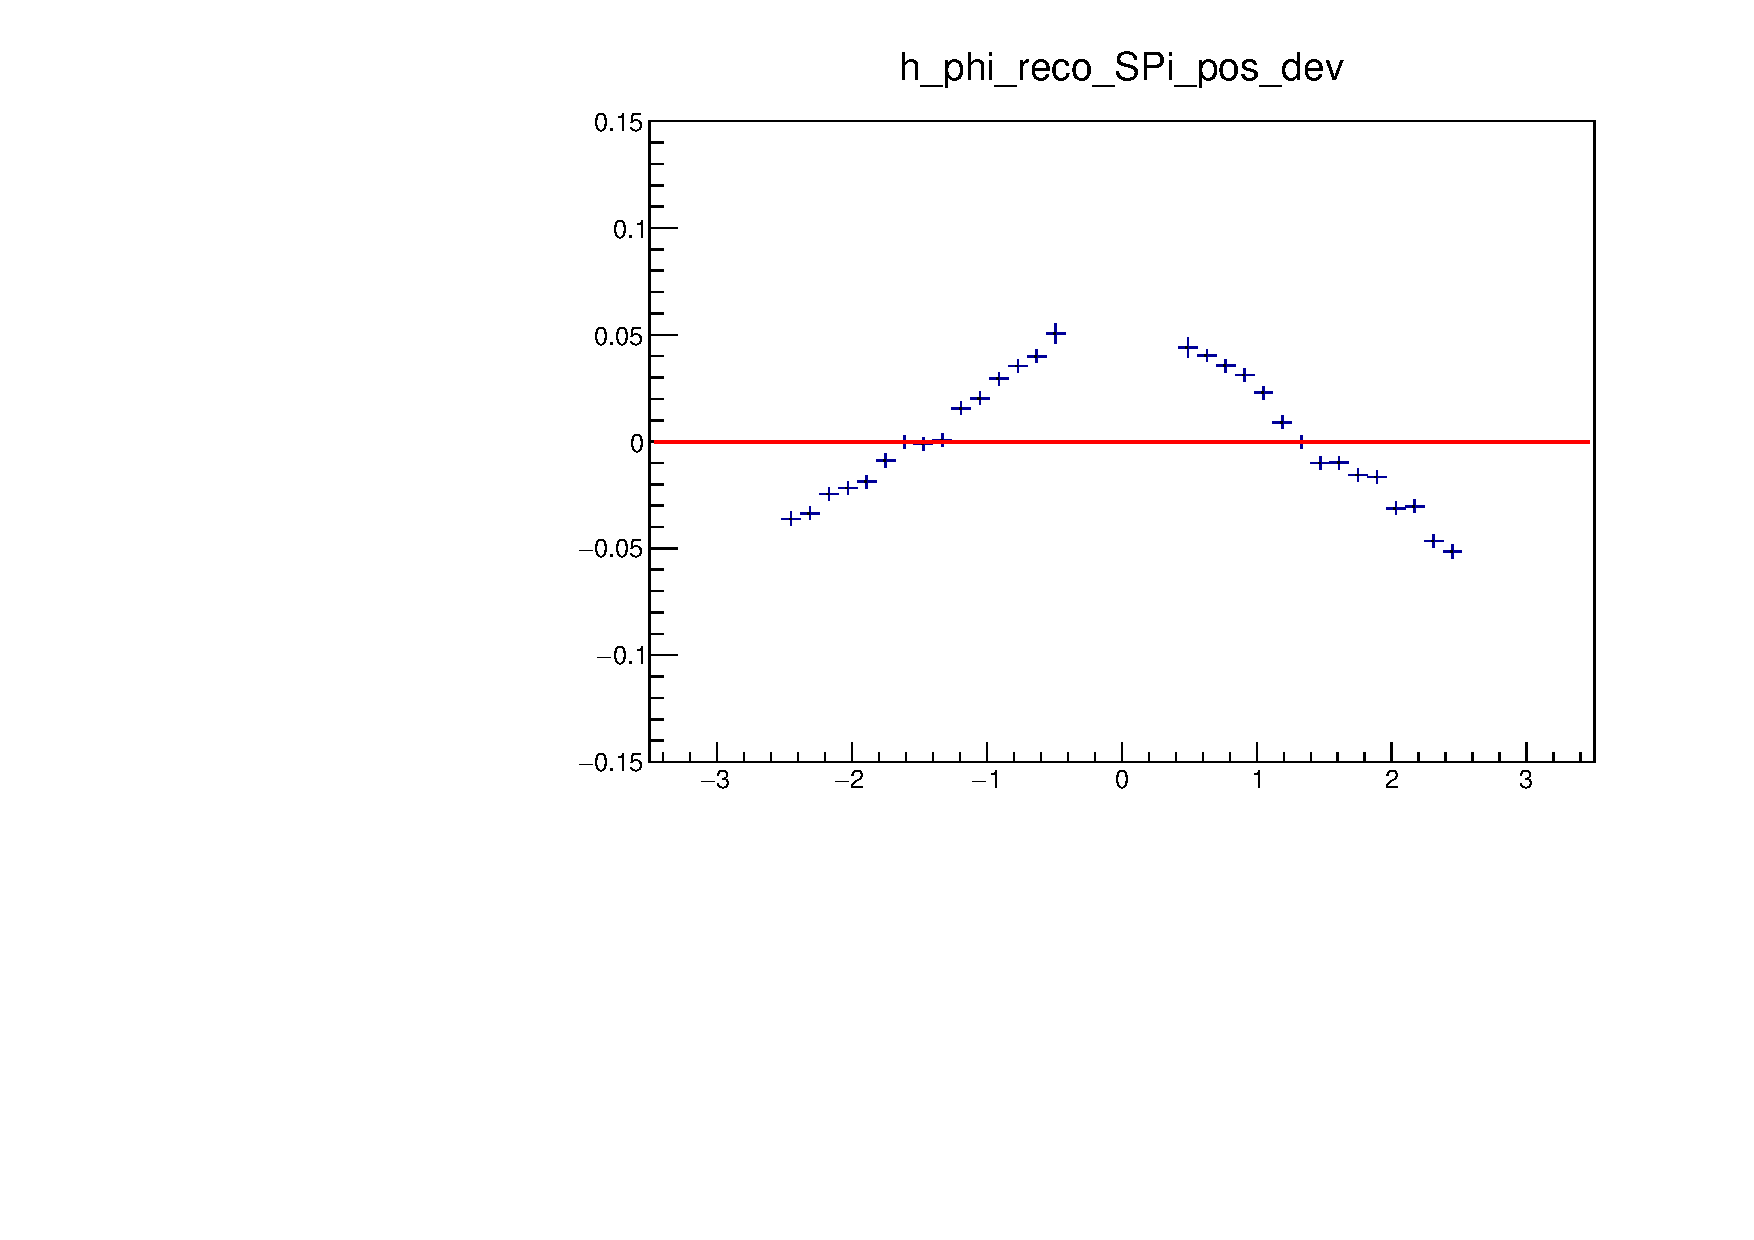
\includegraphics[width=0.9\textwidth]{first/up_pdf/deviation/h_phi_reco_SPi_pos_dev.pdf}
\end{subfigure}
\begin{subfigure}{0.45\textwidth}
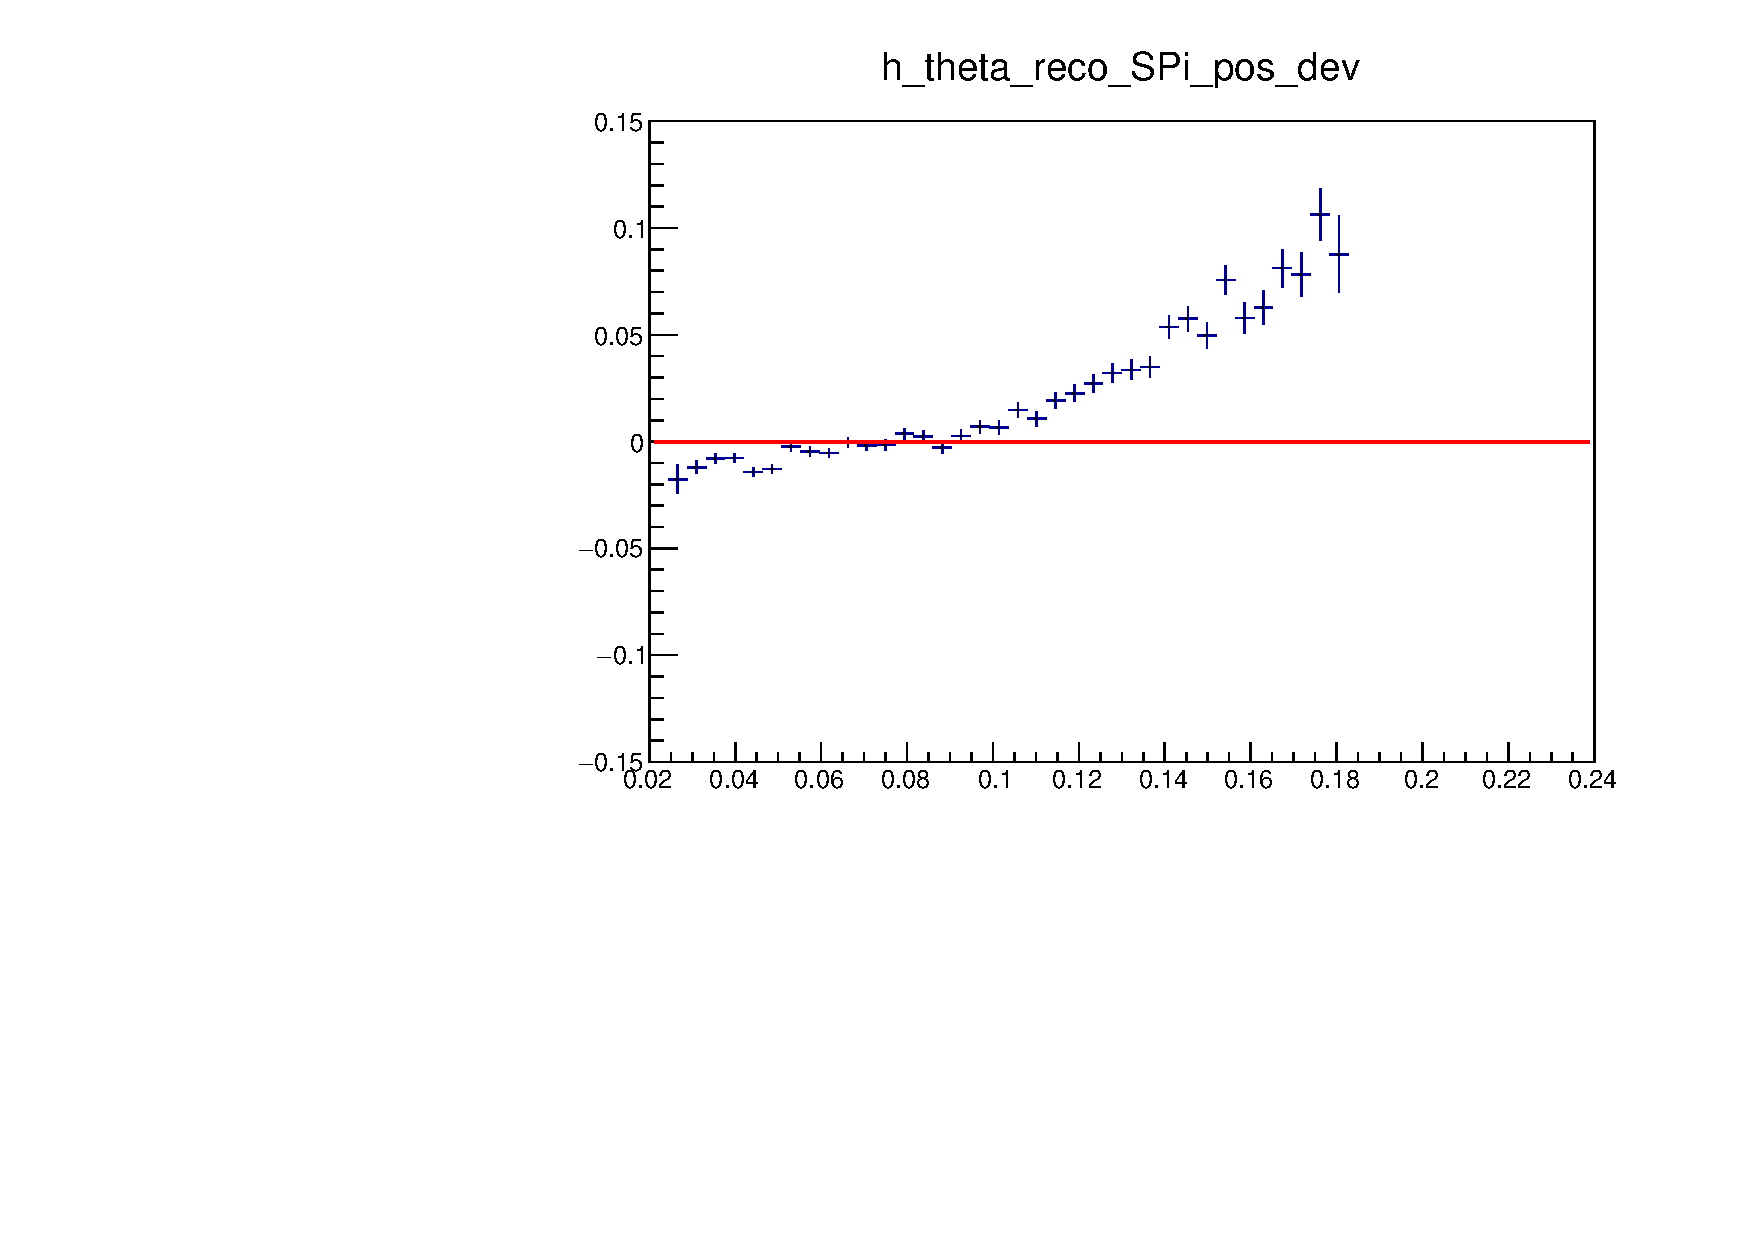
\includegraphics[width=0.9\textwidth]{first/up_pdf/deviation/h_theta_reco_SPi_pos_dev.pdf}
\end{subfigure}
\begin{subfigure}{0.45\textwidth}
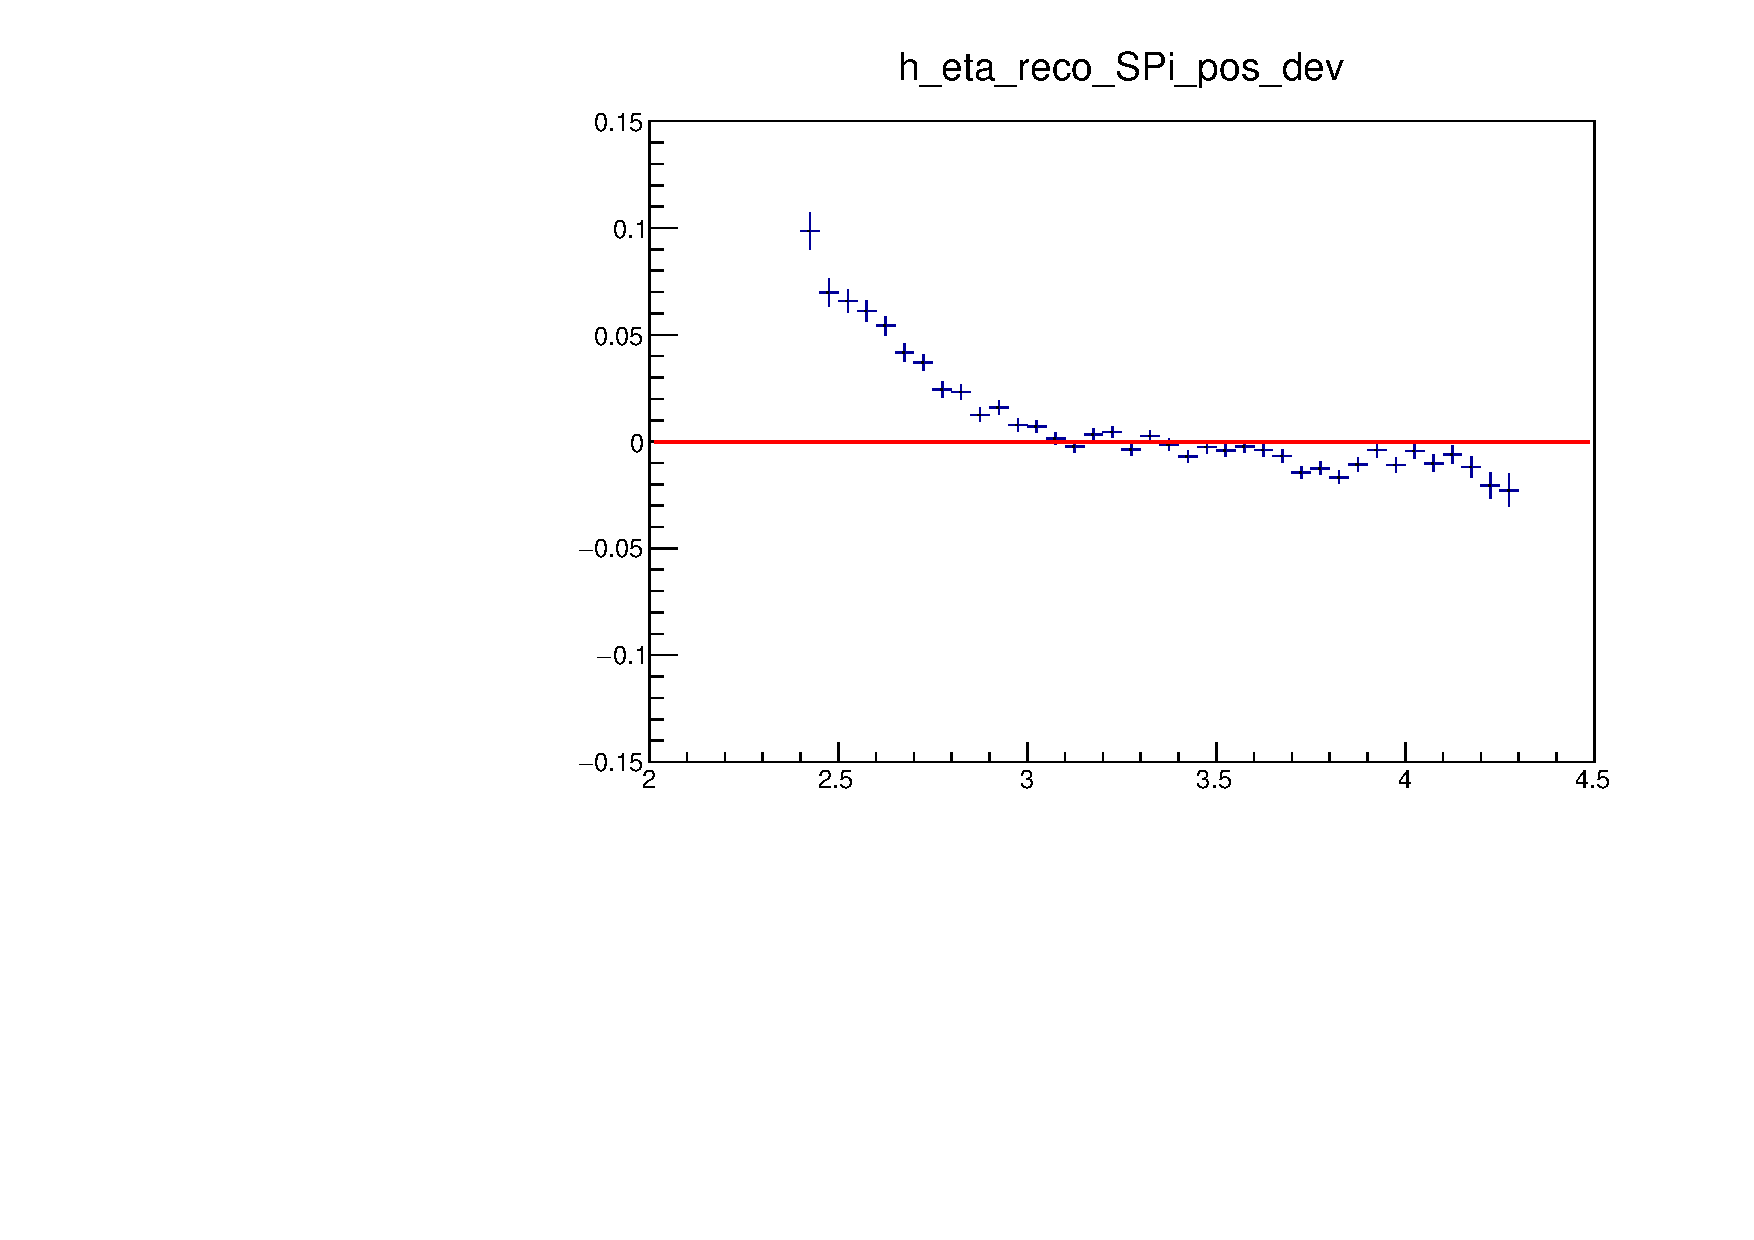
\includegraphics[width=0.9\textwidth]{first/up_pdf/deviation/h_eta_reco_SPi_pos_dev.pdf}
\end{subfigure}
\end{figure}
\end{frame}
\begin{frame}{soft $\pi$ deviation dependencies - $DOWN$ polarity}
\begin{figure}
\begin{subfigure}{0.45\textwidth}
\includegraphics[width=0.9\textwidth]{first/down_pdf/deviation/h_pt_reco_SPi_pos_dev.pdf}
\end{subfigure}
\begin{subfigure}{0.45\textwidth}
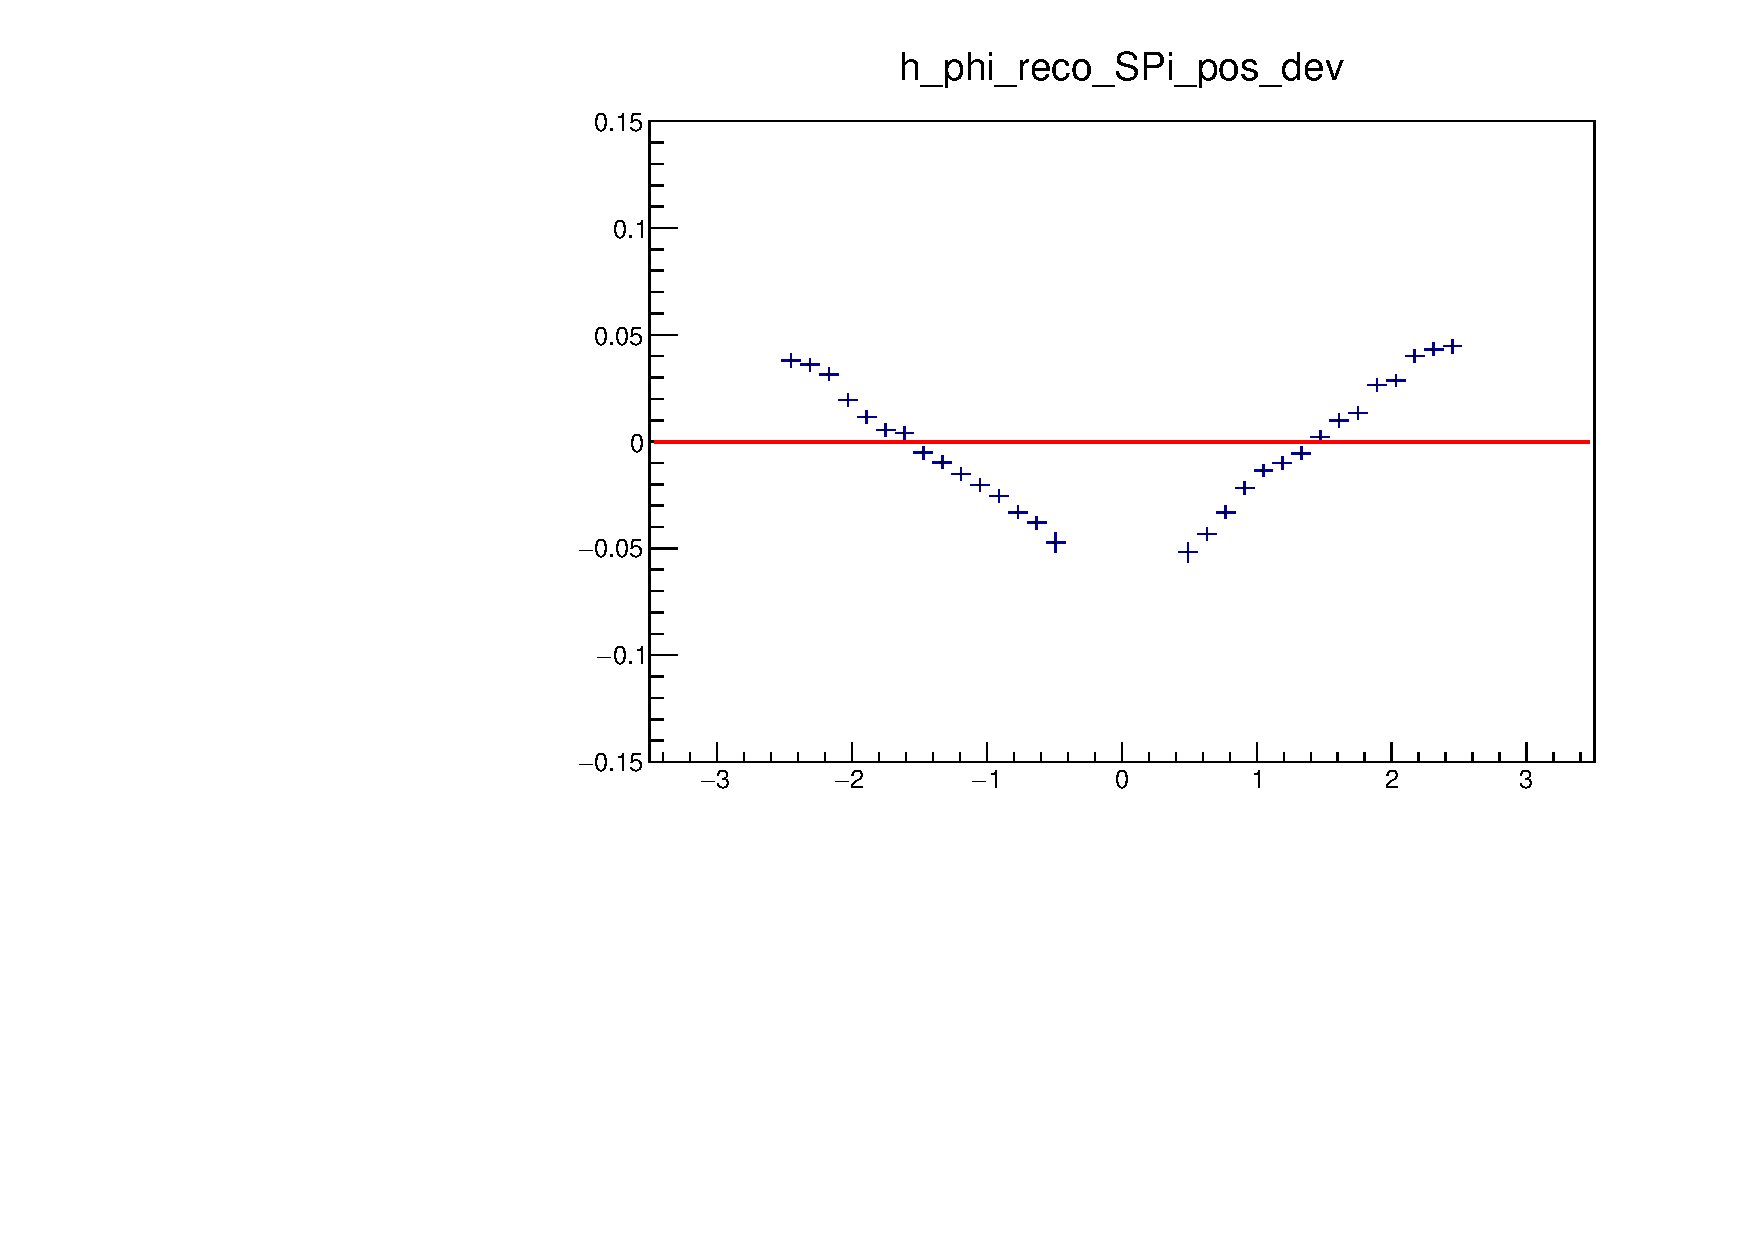
\includegraphics[width=0.9\textwidth]{first/down_pdf/deviation/h_phi_reco_SPi_pos_dev.pdf}
\end{subfigure}
\begin{subfigure}{0.45\textwidth}
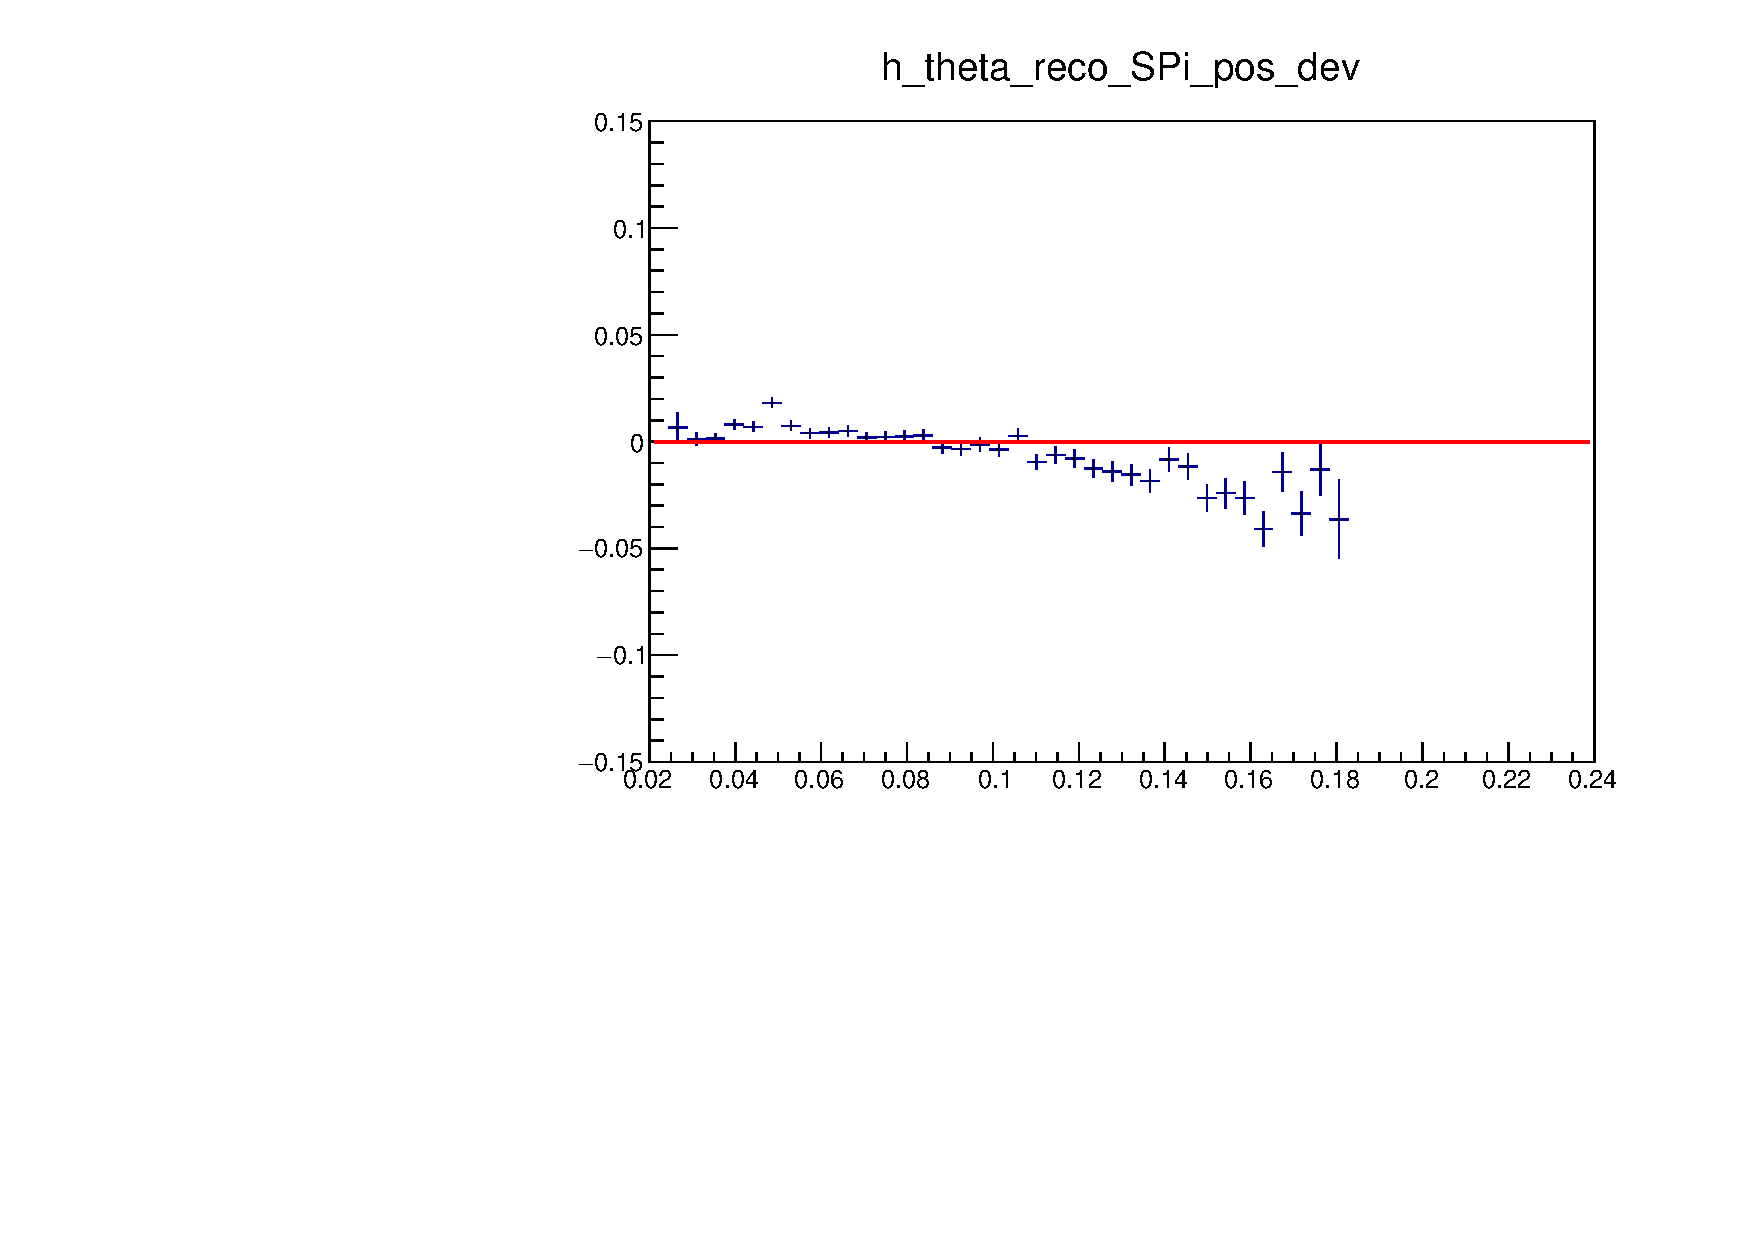
\includegraphics[width=0.9\textwidth]{first/down_pdf/deviation/h_theta_reco_SPi_pos_dev.pdf}
\end{subfigure}
\begin{subfigure}{0.45\textwidth}
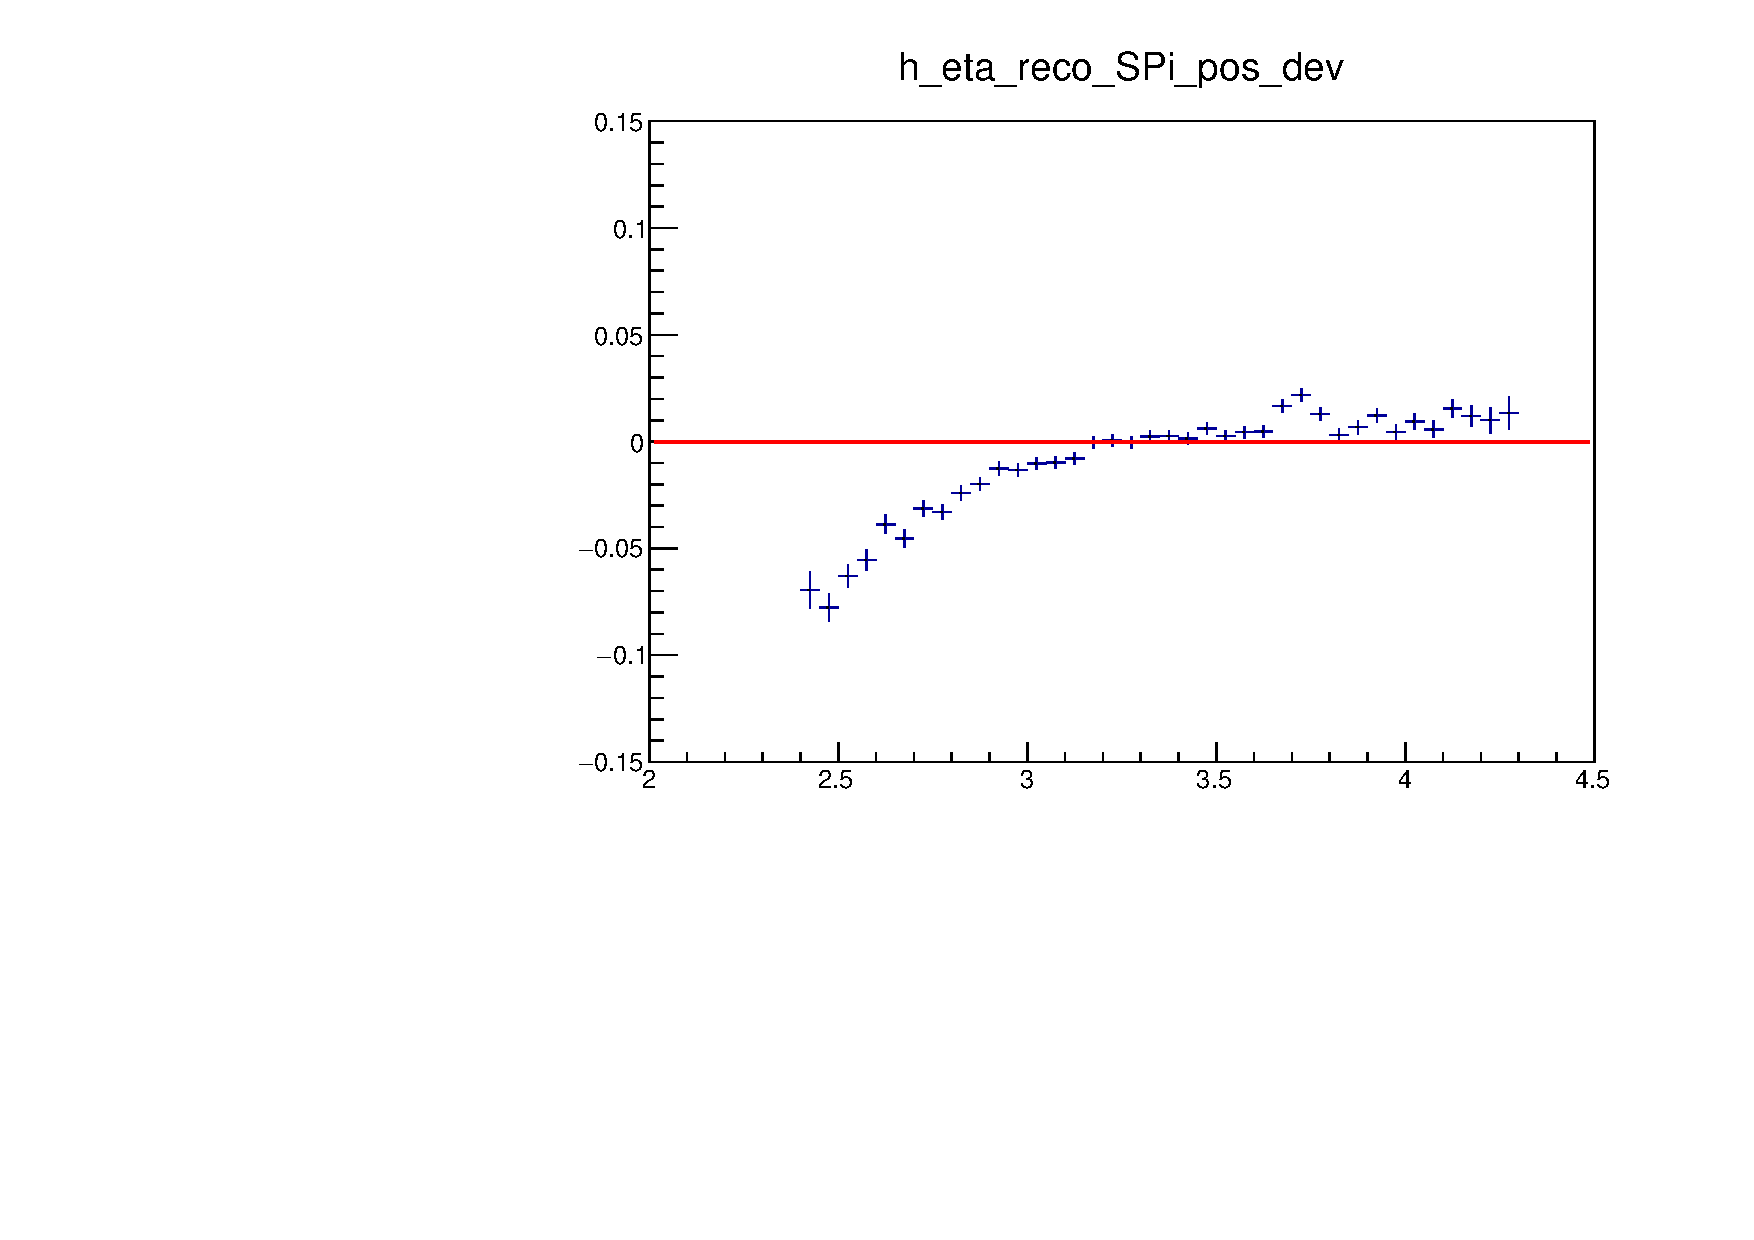
\includegraphics[width=0.9\textwidth]{first/down_pdf/deviation/h_eta_reco_SPi_pos_dev.pdf}
\end{subfigure}
\end{figure}
\end{frame}
\begin{frame}{soft $\pi$ deviation - $\phi$}
\centering
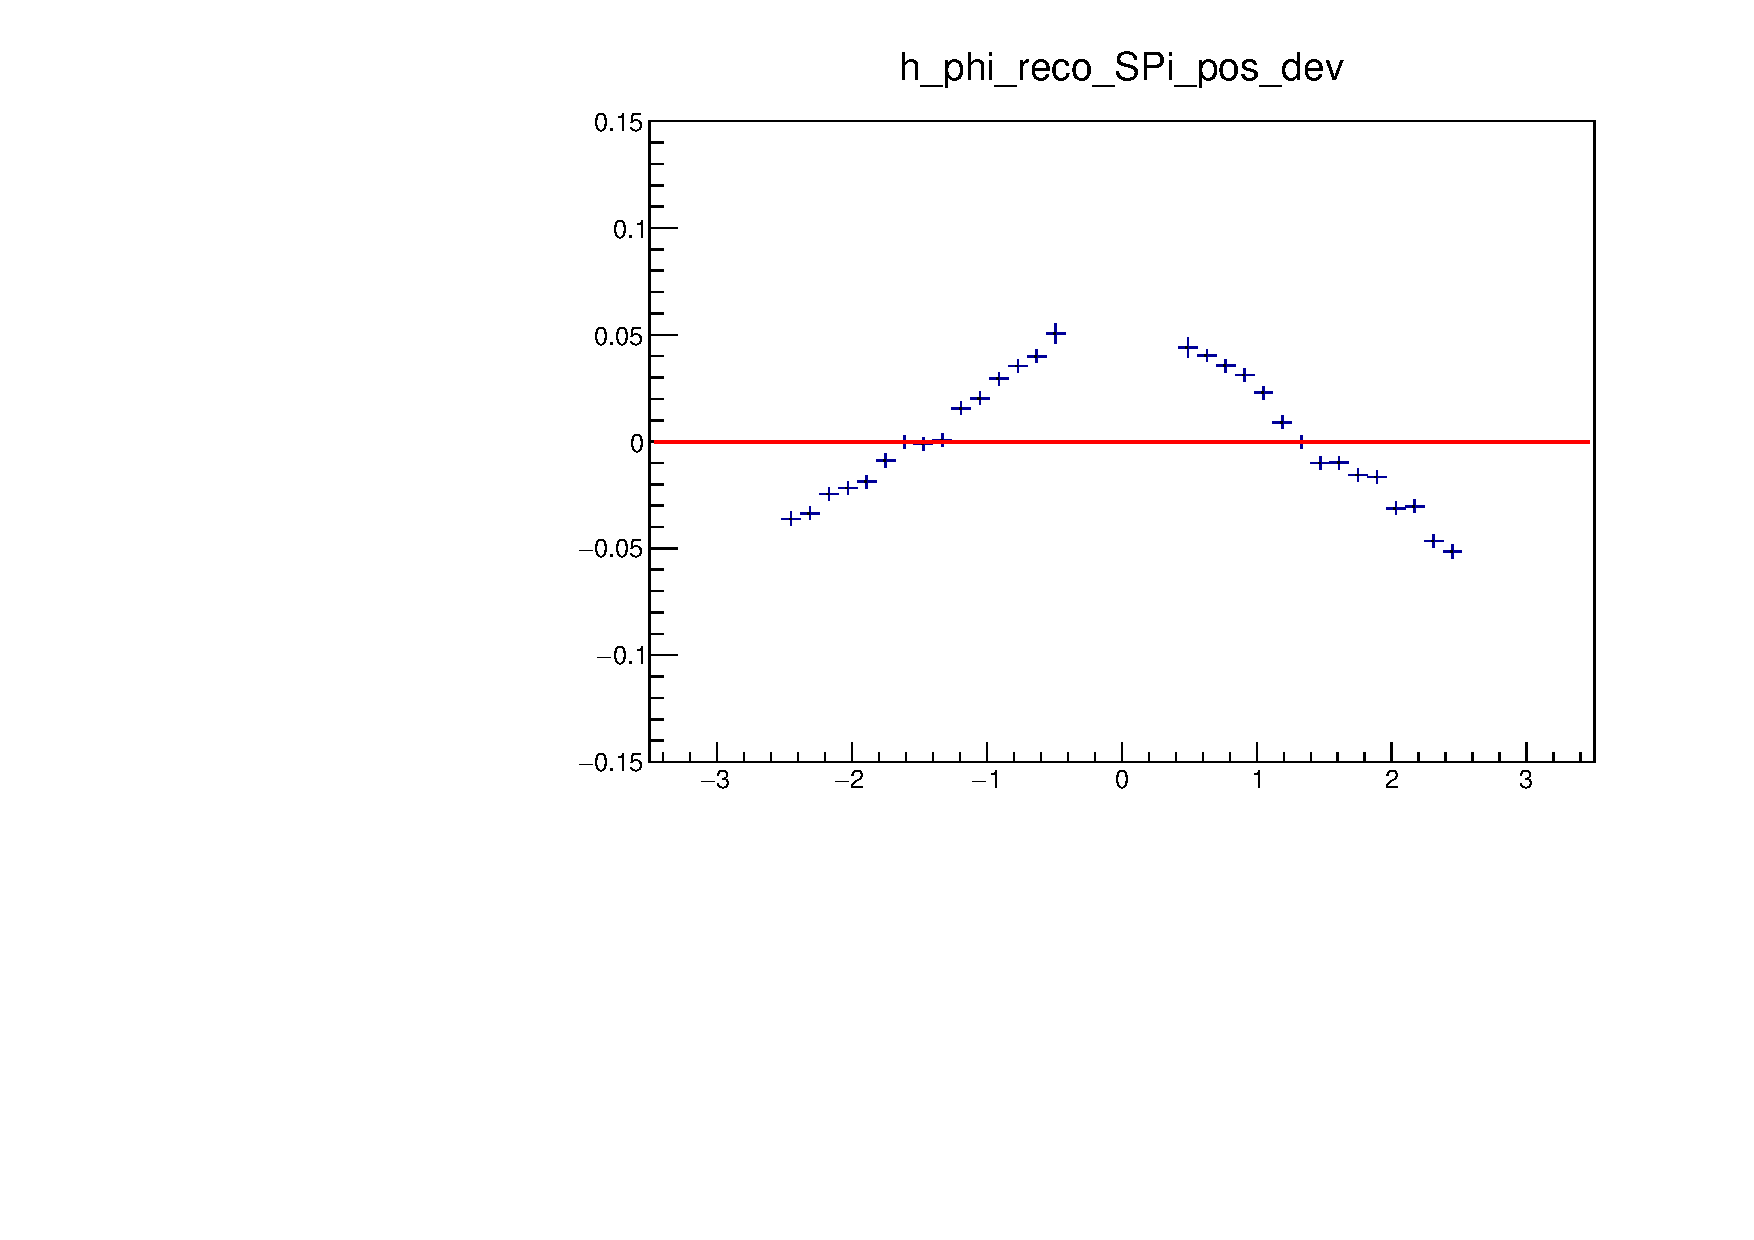
\includegraphics[width=0.48\textwidth]{first/up_pdf/deviation/h_phi_reco_SPi_pos_dev.pdf}
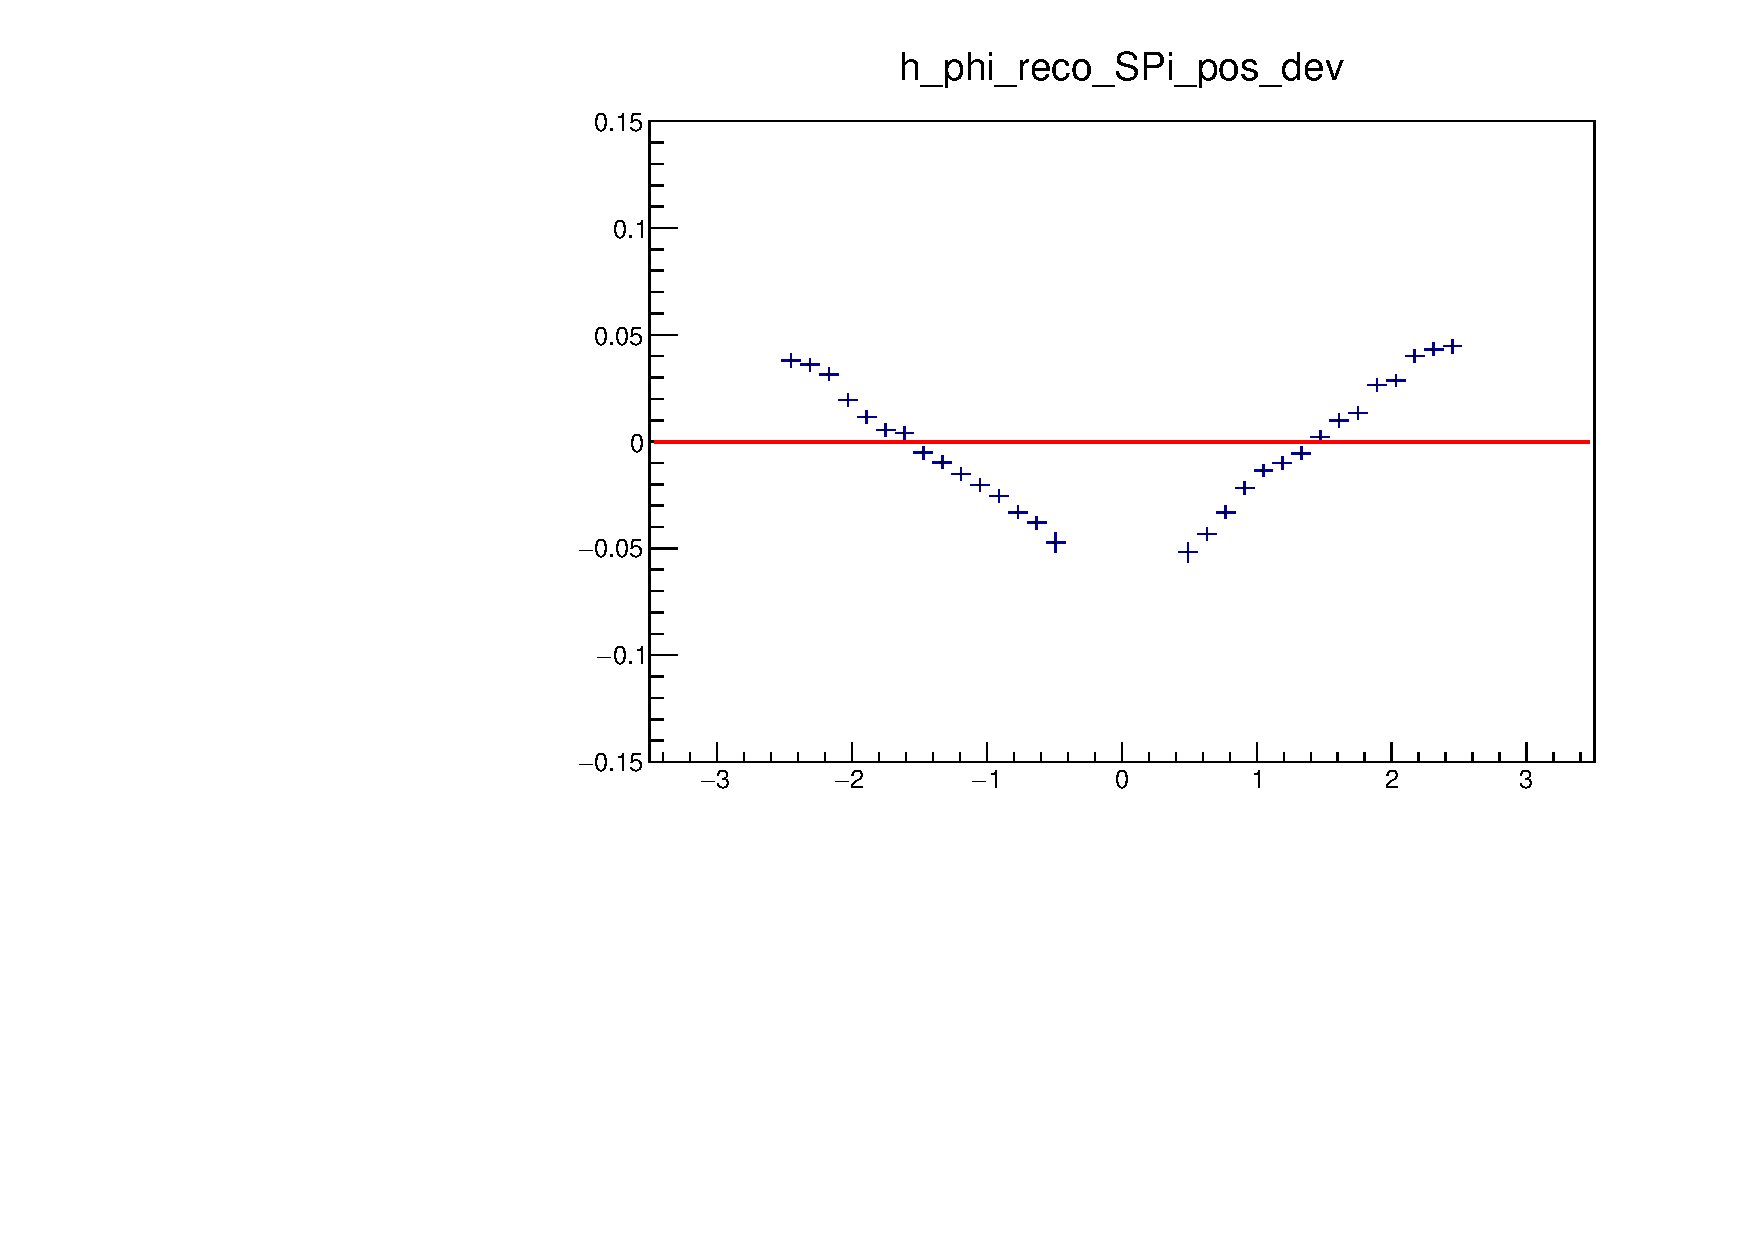
\includegraphics[width=0.48\textwidth]{first/down_pdf/deviation/h_phi_reco_SPi_pos_dev.pdf}
\end{frame}
\begin{frame}{soft $\pi$ deviation UP+DOWN}
\begin{figure}
\begin{subfigure}{0.45\textwidth}
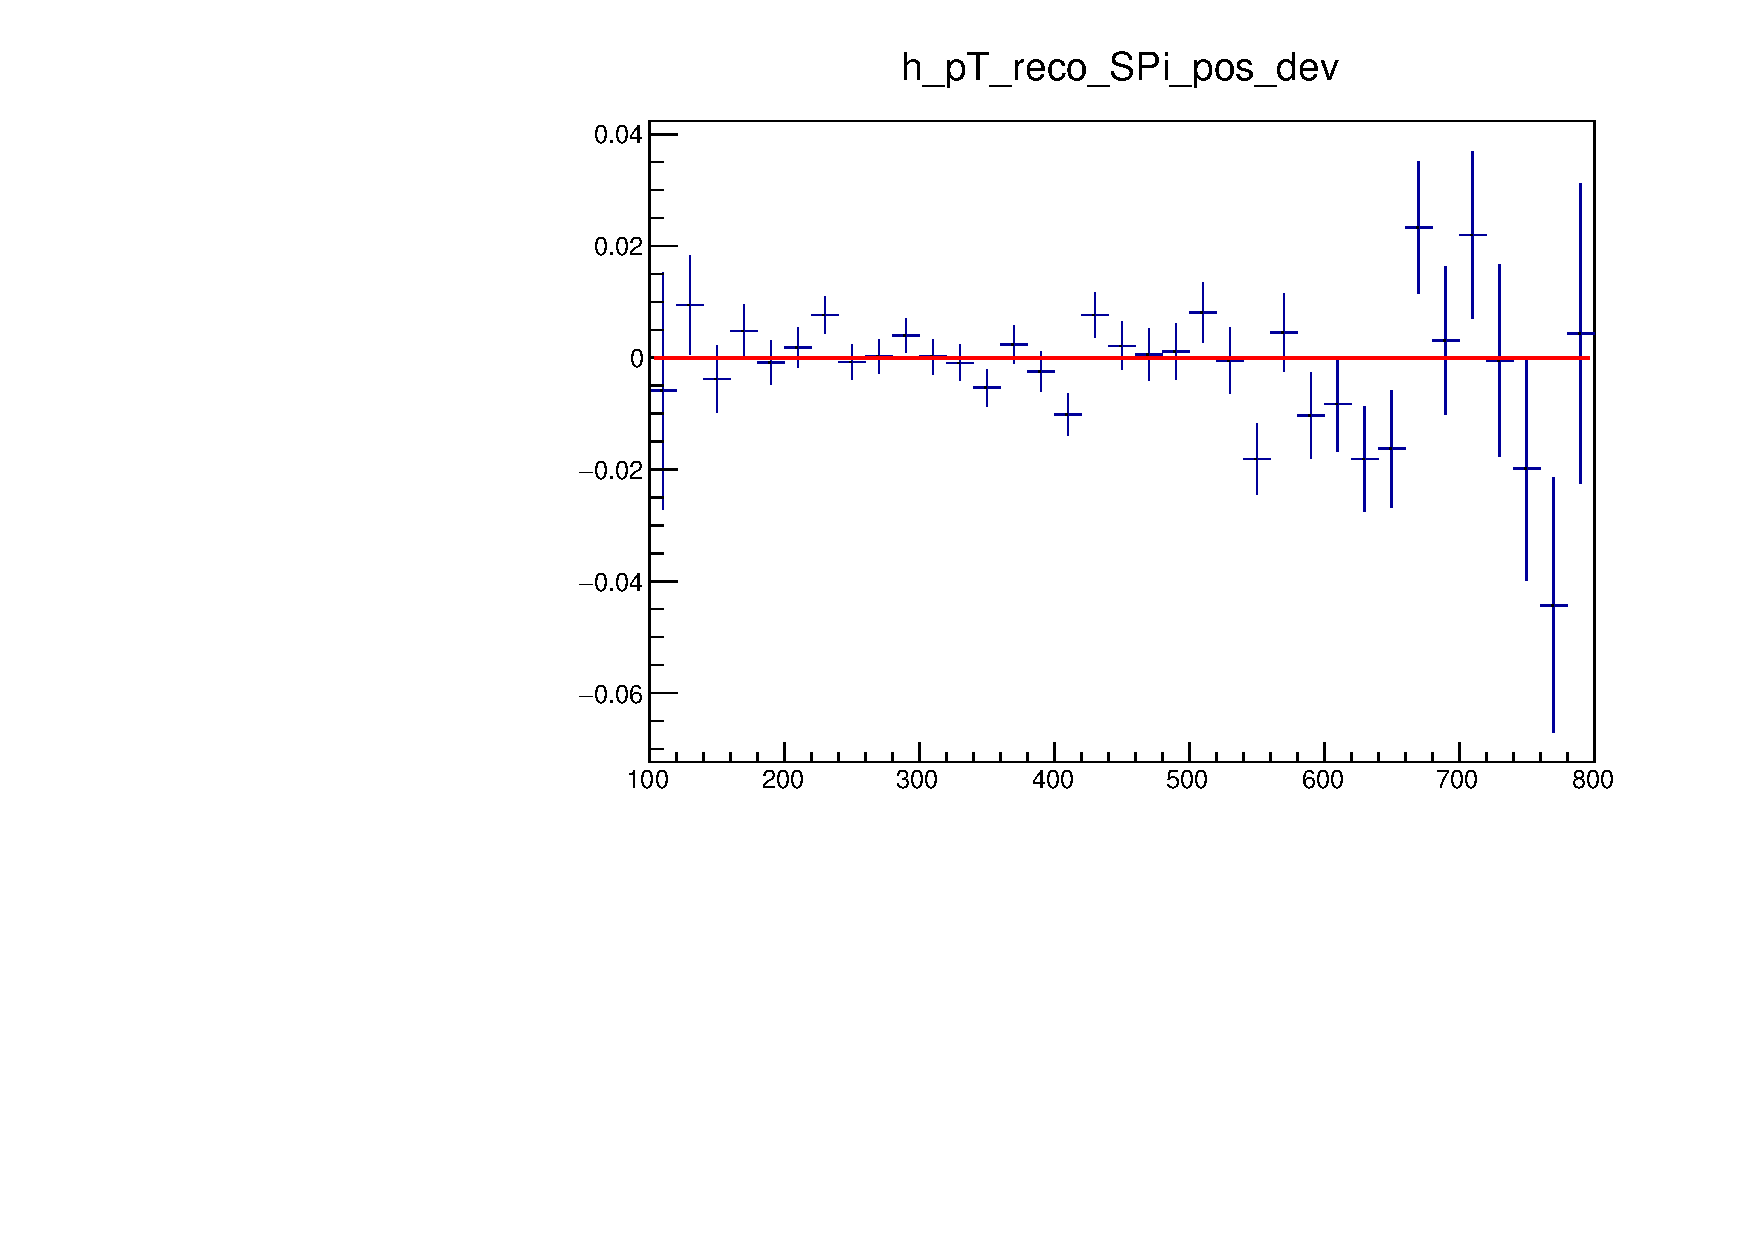
\includegraphics[width=0.9\textwidth]{first/up_plus_down_pdf/pT_2.pdf}
\end{subfigure}
\begin{subfigure}{0.45\textwidth}
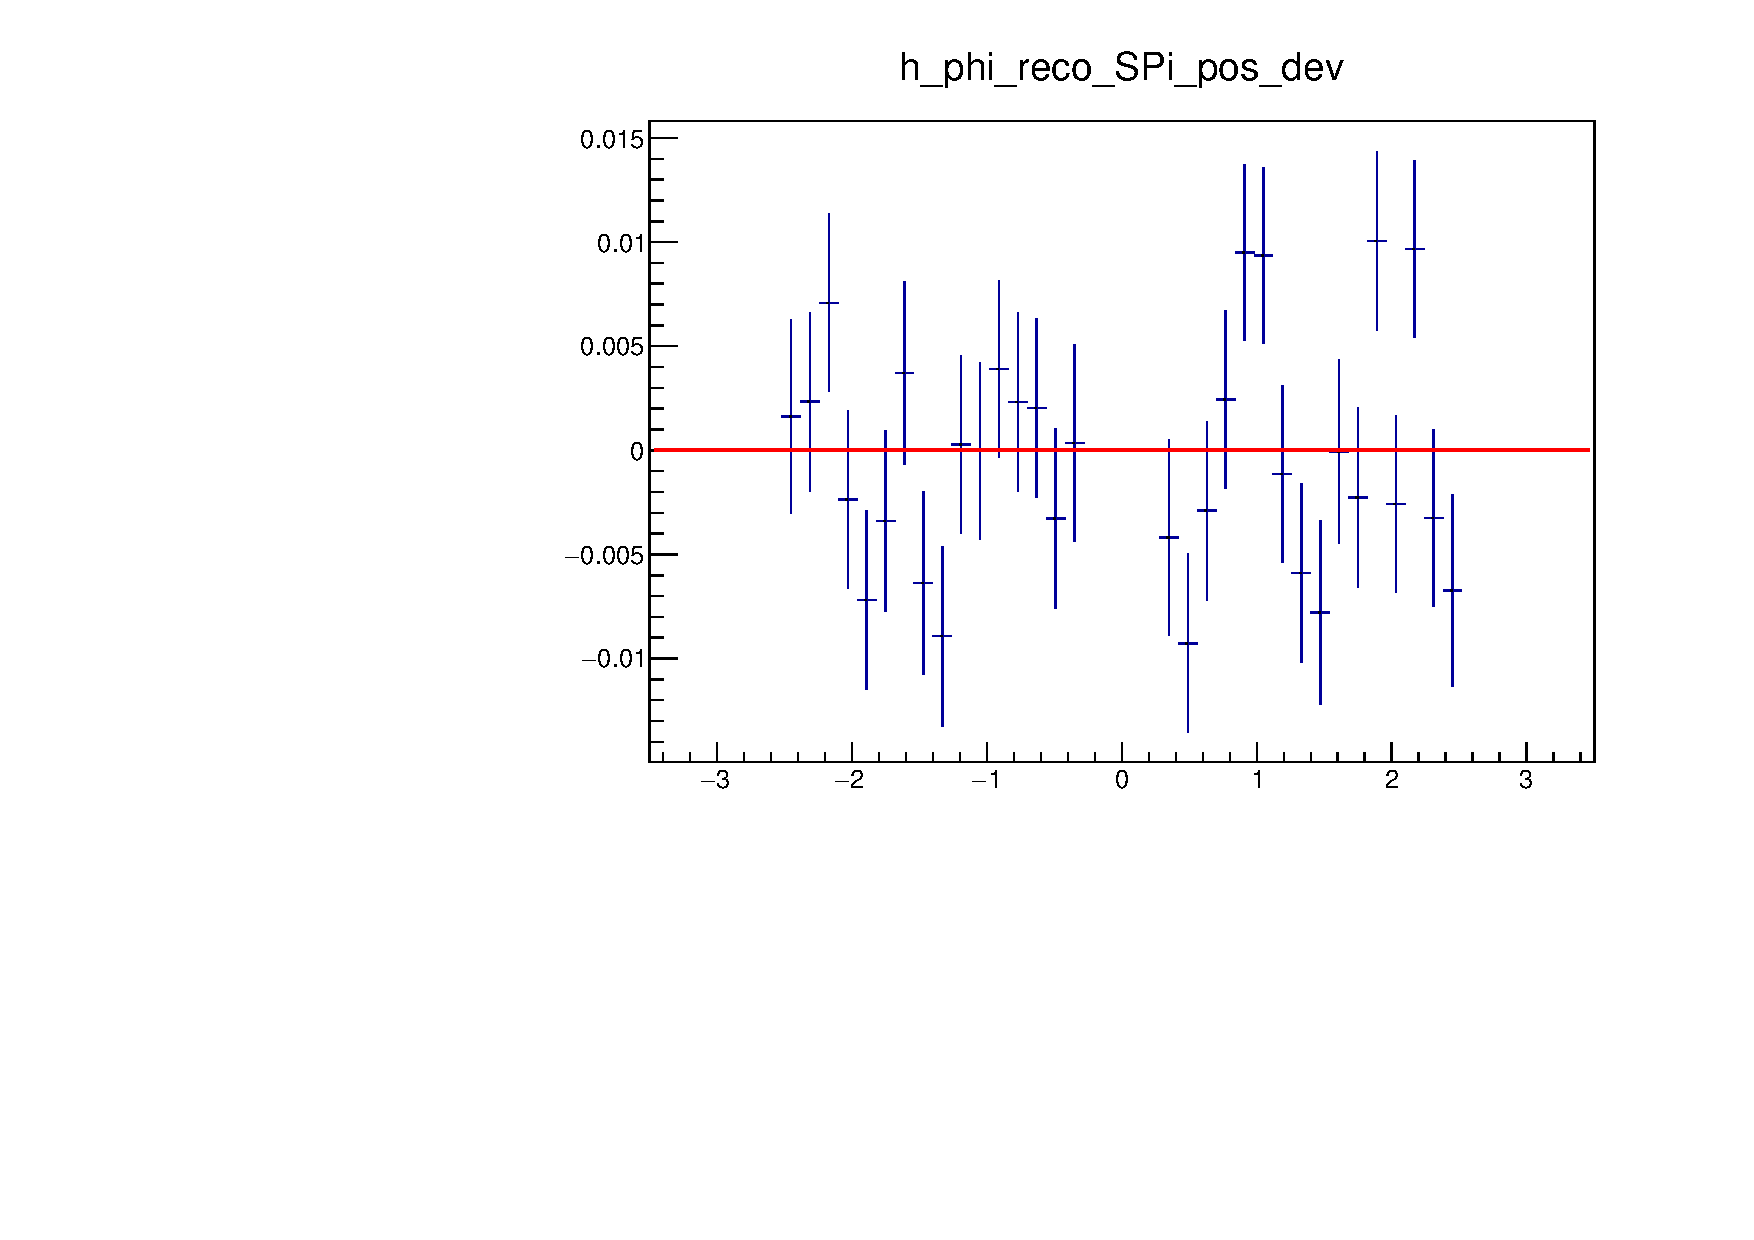
\includegraphics[width=0.9\textwidth]{first/up_plus_down_pdf/phi_2.pdf}
\end{subfigure}
\begin{subfigure}{0.45\textwidth}
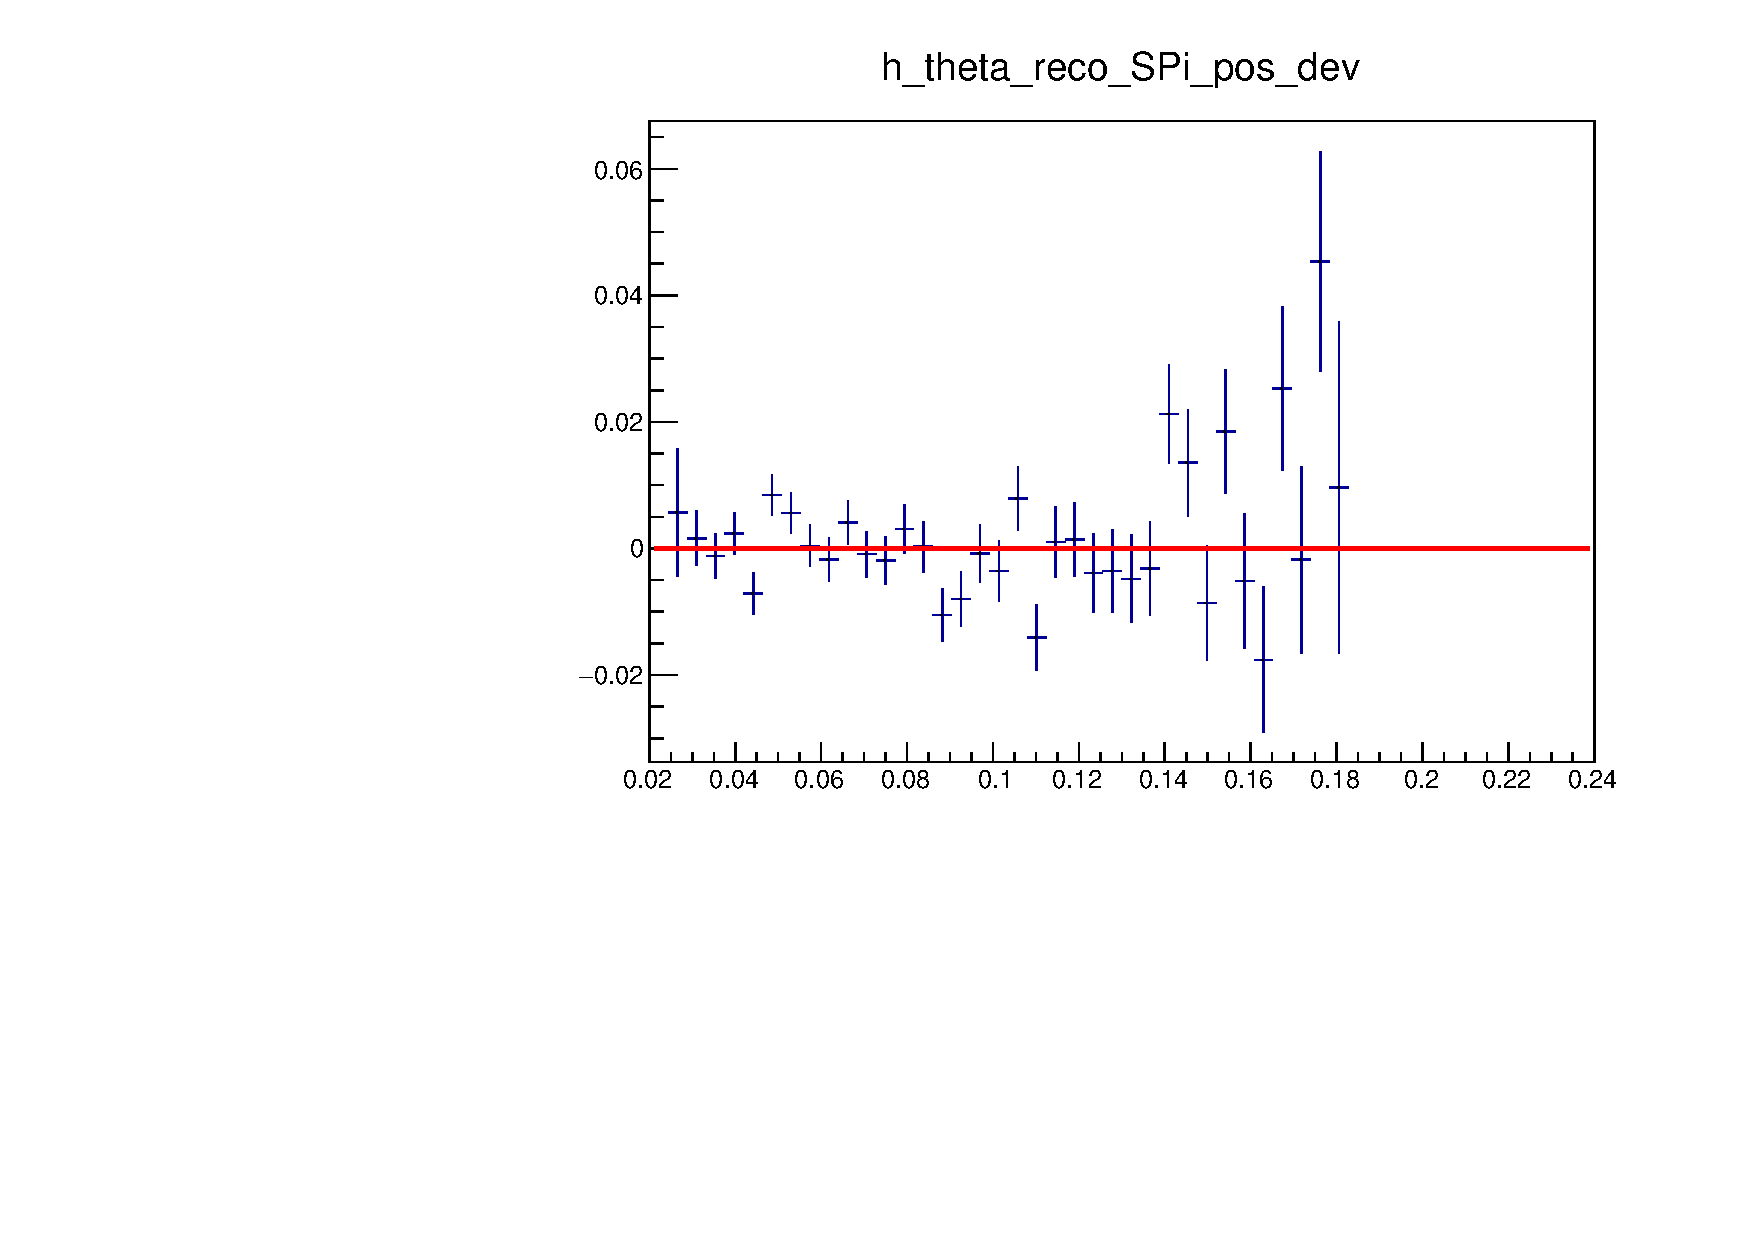
\includegraphics[width=0.9\textwidth]{first/up_plus_down_pdf/theta_2.pdf}
\end{subfigure}
\begin{subfigure}{0.45\textwidth}
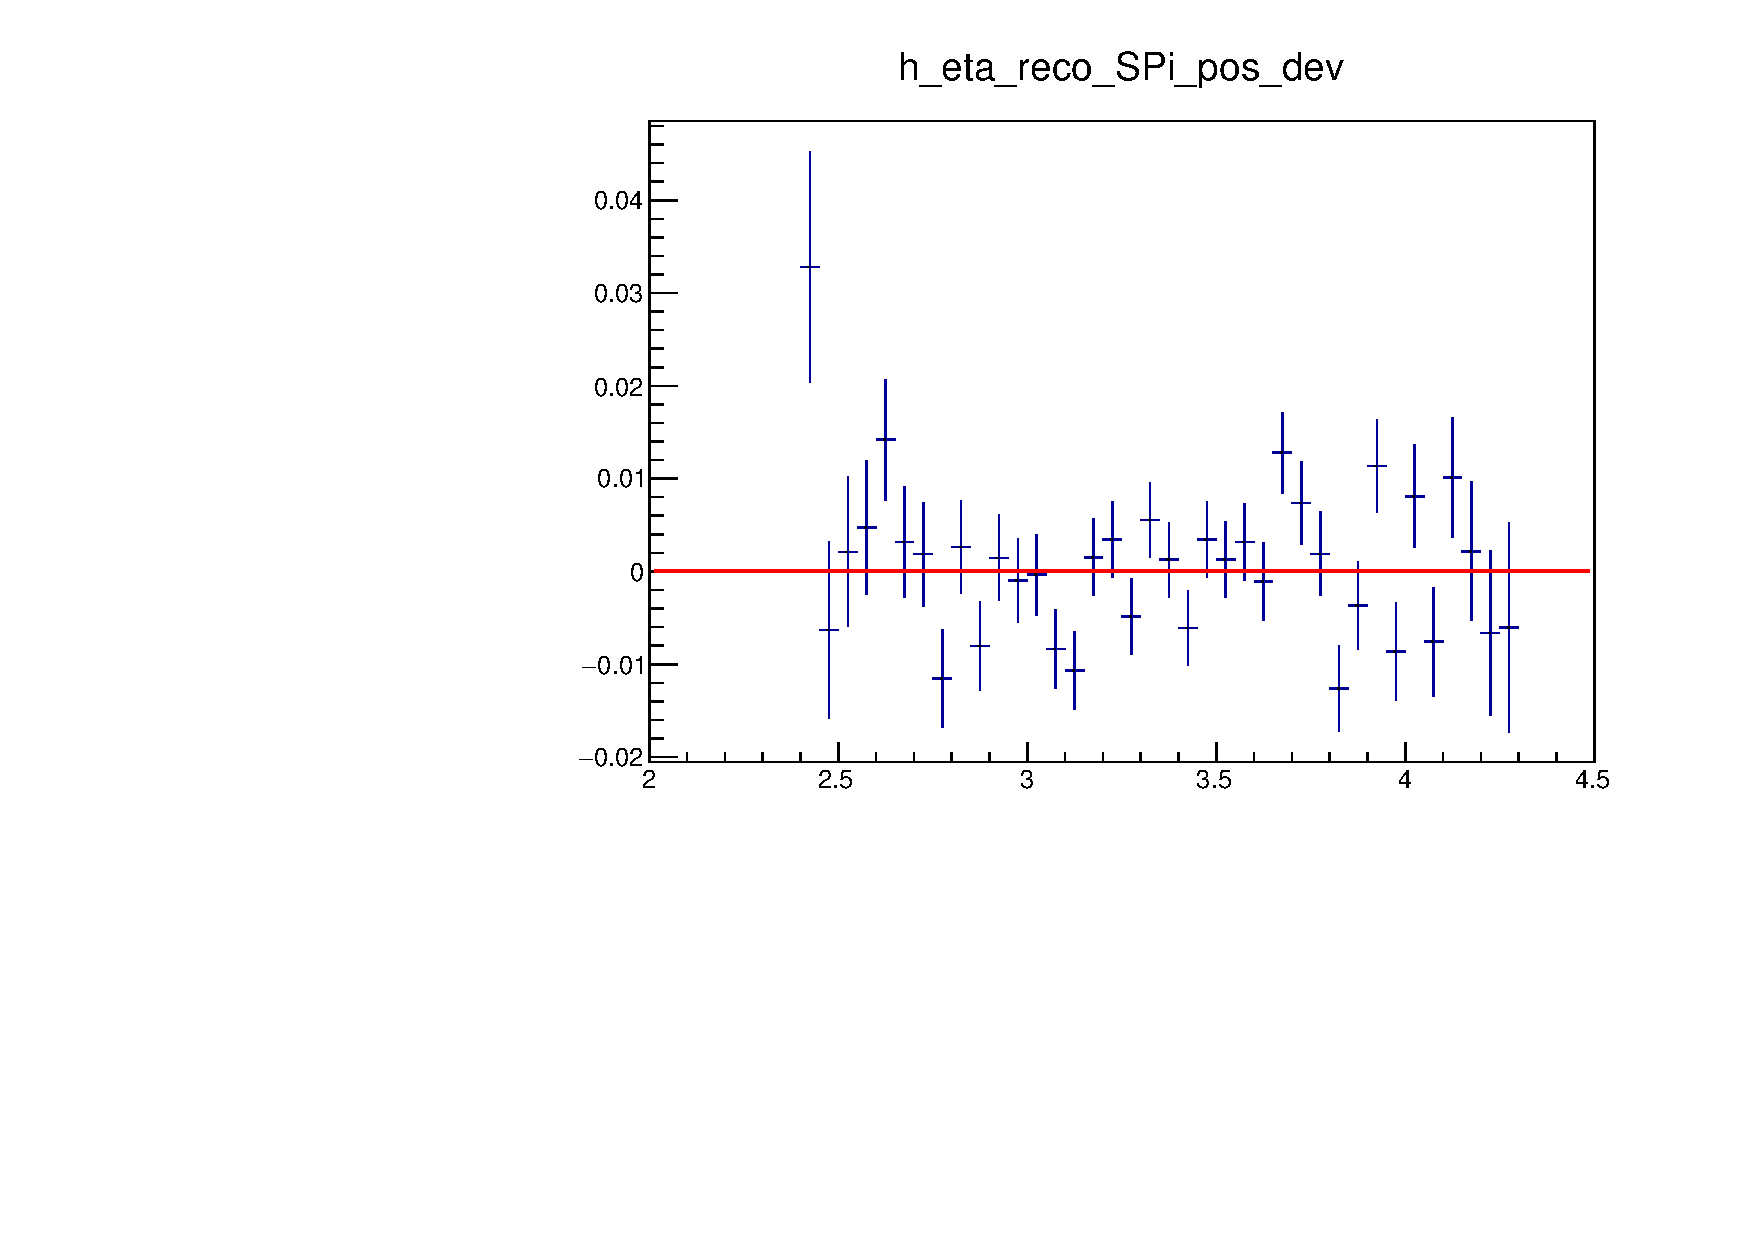
\includegraphics[width=0.9\textwidth]{first/up_plus_down_pdf/eta_2.pdf}
\end{subfigure}
\end{figure}
\end{frame}
\begin{frame}{Idea 2}
\begin{itemize}
\item $|\phi| < 0.3 \& |\phi| > 2.5$ \& $\eta > 3$
\end{itemize}
\begin{figure}
\begin{subfigure}{0.45\textwidth}
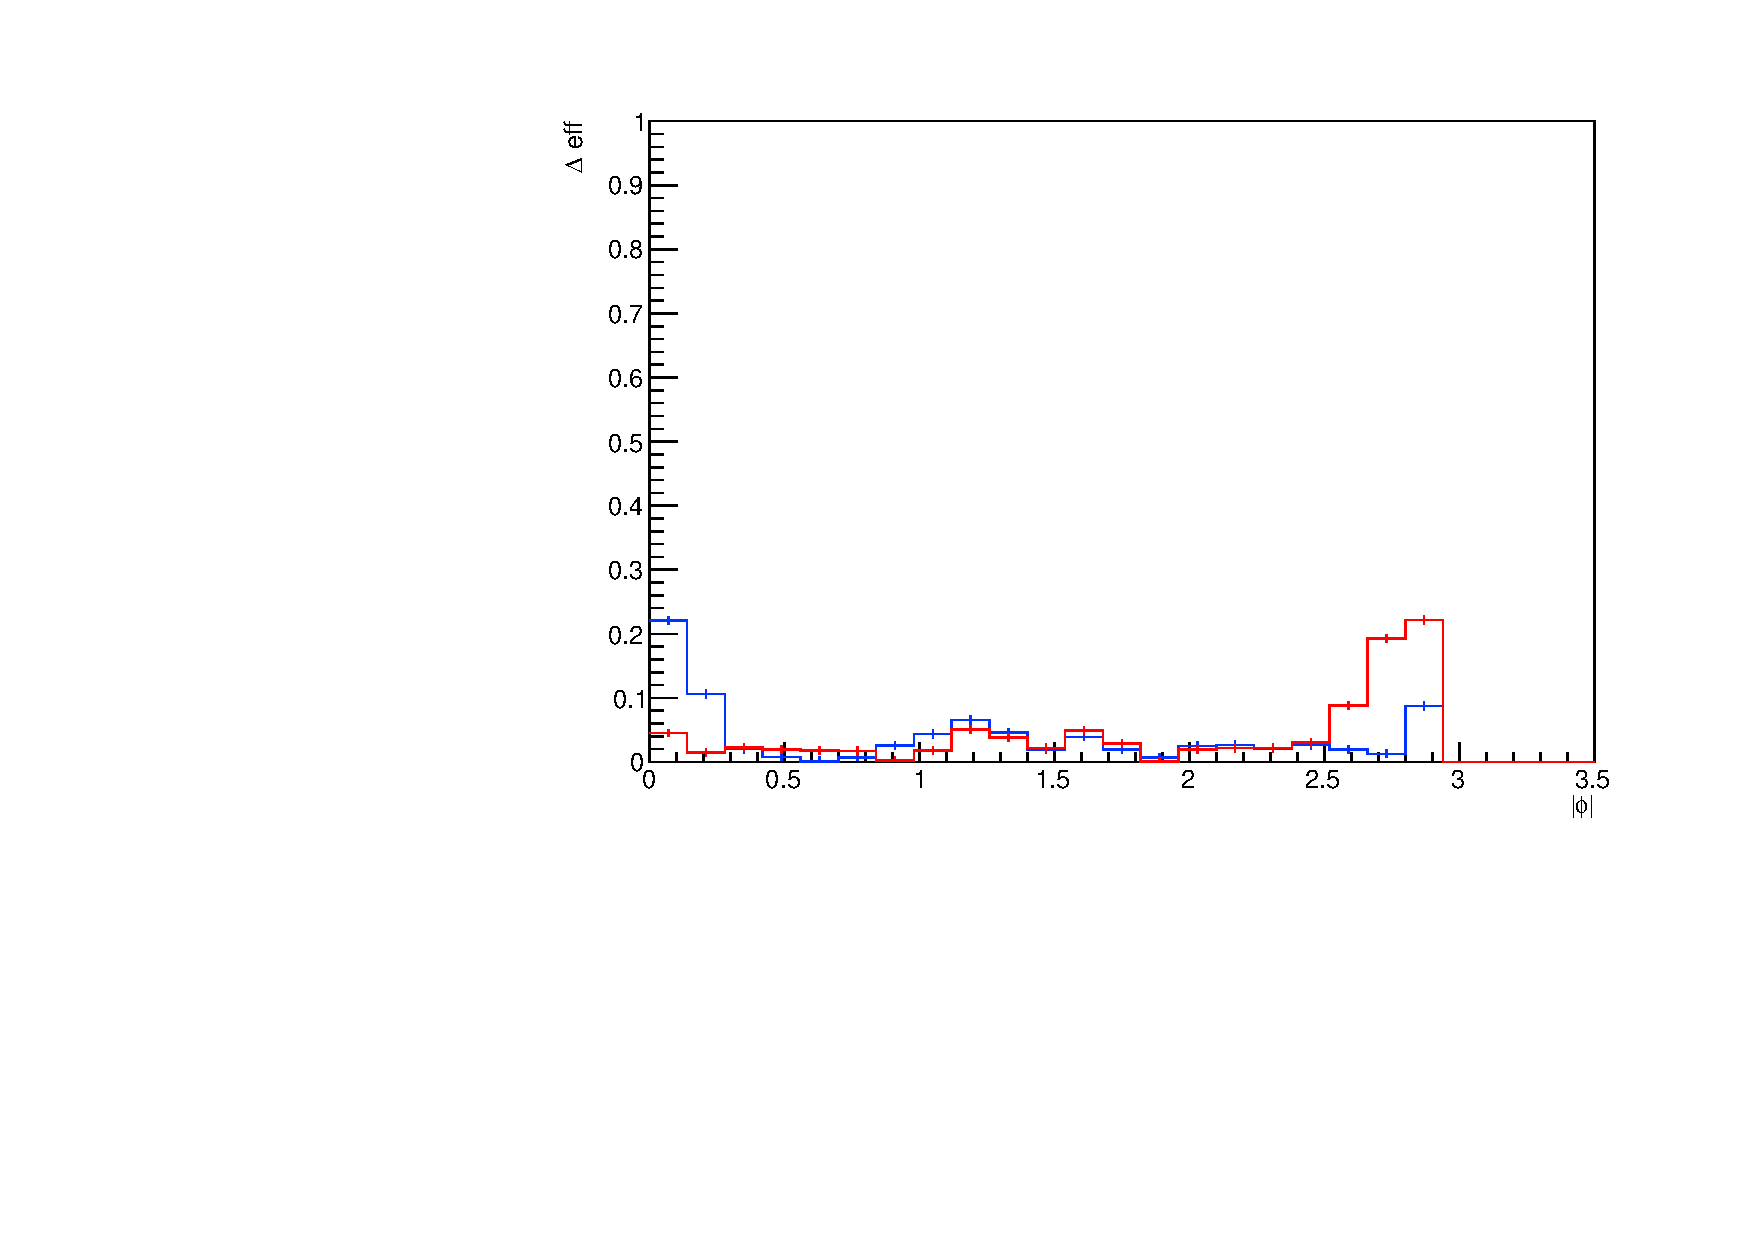
\includegraphics[width=0.9\textwidth]{first/up_pdf/test_u/h_phi_test_SPi_combined.pdf}
\end{subfigure}
\begin{subfigure}{0.45\textwidth}
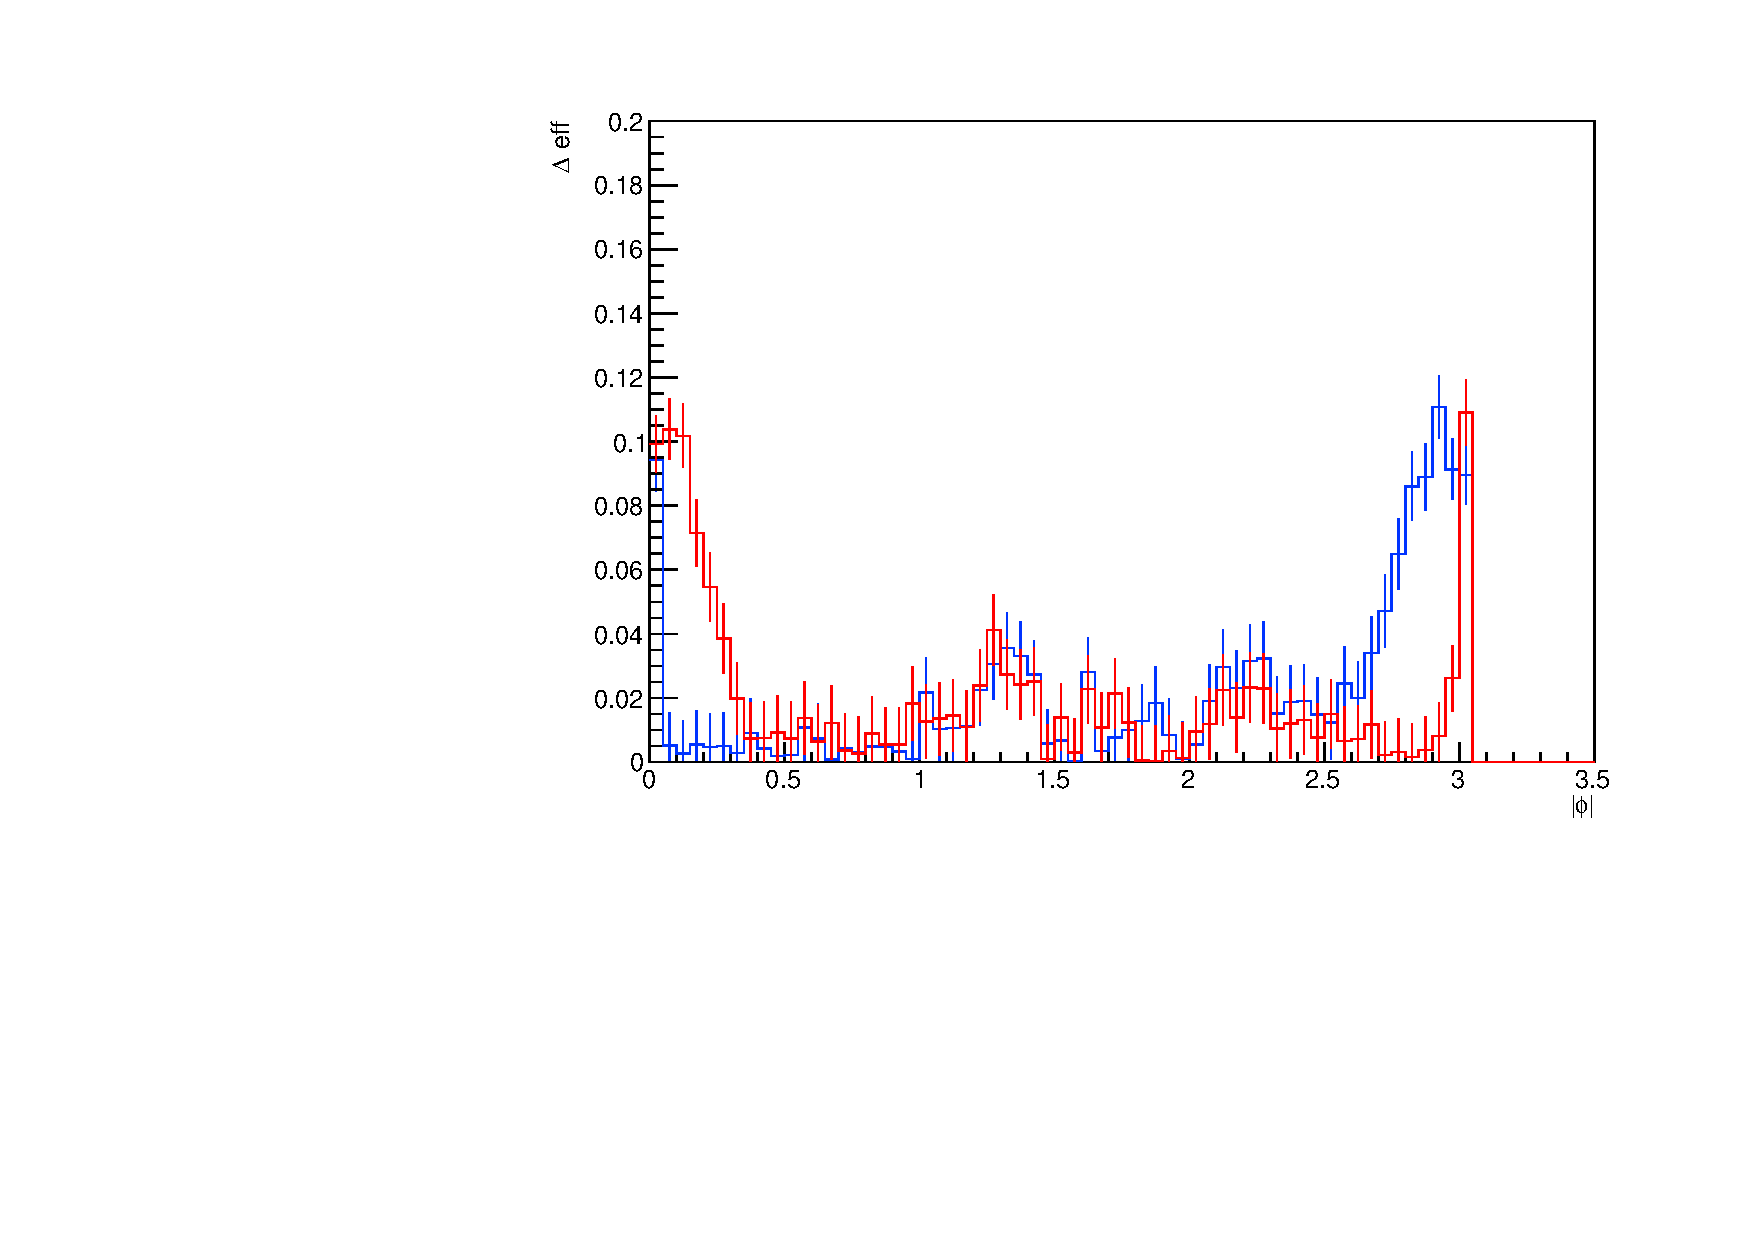
\includegraphics[width=0.9\textwidth]{first/down_pdf/test_d/h_phi_test_SPi_combined.pdf}
\end{subfigure}
\end{figure}
\end{frame}
%\begin{frame}{Total Efficiencies - before cut}
%\begin{table}
%\resizebox{\textwidth}{!}{
%	\begin{tabular}{cS[table-format=2.2]@{${}\pm{}$}S[table-format=1.2]S[table-format=2.2]@{${}\pm{}$}S[table-format=1.2]S[table-format=2.2]@{${}\pm{}$}S[table-format=1.2]S[table-format=2.2]@{${}\pm{}$}S[table-format=1.2]S[table-format=2.2]@{${}\pm{}$}S[table-format=1.2]}
%		\toprule
%		{Polarity} & \multicolumn{2}{c}{$\epsilon_{\pi} $} & \multicolumn{2}{c}{$\epsilon_{K} $} & \multicolumn{2}{c}{$ \epsilon_{\pi,s} $} & \multicolumn{2}{c}{$\epsilon_{D^0} $} & \multicolumn{2}{c}{$\epsilon_{D^*} $} \\
%		\midrule
%		$UP$ & 86.65 & 0.01 & 84.63 & 0.01 & 76.65 & 0.02 & 73.34 & 0.02 & 56.31 & 0.02\\
%		$DOWN$ & 86.68 & 0.01 & 84.67 & 0.01 & 76.66 & 0.02 & 73.39 & 0.02 & 56.35 & 0.02\\
%		\bottomrule
%	\end{tabular}}
%\end{table}
%\end{frame}
%
%\begin{frame}{Total Efficiencies - after cut}
%\begin{table}
%\resizebox{\textwidth}{!}{
%	\begin{tabular}{cS[table-format=2.2]@{${}\pm{}$}S[table-format=1.2]S[table-format=2.2]@{${}\pm{}$}S[table-format=1.2]S[table-format=2.2]@{${}\pm{}$}S[table-format=1.2]S[table-format=2.2]@{${}\pm{}$}S[table-format=1.2]S[table-format=2.2]@{${}\pm{}$}S[table-format=1.2]}
%		\toprule
%		{Polarity} & \multicolumn{2}{c}{$\epsilon_{\pi} $} & \multicolumn{2}{c}{$\epsilon_{K} $} & \multicolumn{2}{c}{$ \epsilon_{\pi,s} $} & \multicolumn{2}{c}{$\epsilon_{D^0} $} & \multicolumn{2}{c}{$\epsilon_{D^*} $} \\
%		\midrule
%		$UP$ & 86.65 & 0.01 & 84.63 & 0.01 & 50.23 & 0.02 & 73.34 & 0.02 & 36.61 & 0.02\\
%		$DOWN$ & 86.68 & 0.01 & 84.67 & 0.01 & 42.87 & 0.02 & 73.39 & 0.02 & 31.29 & 0.02\\
%		\bottomrule
%	\end{tabular}}
%\end{table}
%\end{frame}
%\begin{frame}
%\begin{LARGE}
%\textbf{Charge: +}
%\end{LARGE}
%\end{frame}
%\begin{frame}{Numbers - before cut}
%\begin{table}
%\resizebox{\textwidth}{!}{
%%	\caption{UP Polarity - reconstructed vs. total number of events}
%	\begin{tabular}{cS[table-format=6.0]S[table-format=6.0]S[table-format=6.0]S[table-format=6.0]S[table-format=6.0]}
%		\toprule
%		{UP} & {$\pi $} & {$K $} & {$ soft\, \pi $} & {$D^0 $} & {$D^* $} \\
%		\midrule
%		$N_\text{reco}$ & 2669990 & 2620280 & 2352910 & 2249370 & 1720940 \\
%		$N_\text{tot}$ & 3000000 & 3000000 & 3000000 & 3000000 & 3000000 \\
%		\bottomrule
%	\end{tabular}}
%\resizebox{\textwidth}{!}{
%%	\caption{DOWN Polarity - reconstructed vs. total number of events}
%	\begin{tabular}{cS[table-format=6.0]S[table-format=6.0]S[table-format=6.0]S[table-format=6.0]S[table-format=6.0]}
%		\toprule
%		{DOWN} & {$\pi $} & {$K $} & {$ soft\, \pi $} & {$D^0 $} & {$D^* $} \\
%		\midrule
%		$N_\text{reco}$ & 2674000 & 2626350 & 2374360 & 2253370 & 1737460 \\
%		$N_\text{tot}$ & 3000000 & 3000000 & 3000000 & 3000000 & 3000000 \\
%		\bottomrule
%	\end{tabular}}
%\end{table}
%\end{frame}
%\begin{frame}{Numbers - after cut}
%\begin{table}
%\resizebox{\textwidth}{!}{
%%	\caption{UP Polarity - reconstructed vs. total number of events}
%	\begin{tabular}{cS[table-format=6.0]S[table-format=6.0]S[table-format=6.0]S[table-format=6.0]S[table-format=6.0]}
%		\toprule
%		{UP} & {$\pi $} & {$K $} & {$ soft\, \pi $} & {$D^0 $} & {$D^* $} \\
%		\midrule
%		$N_\text{reco}$ & 2669990 & 2620280 & 1546670 & 2249370 & 1121530 \\
%		$N_\text{tot}$ & 3000000 & 3000000 & 1961330 & 3000000 & 1961330 \\
%		\bottomrule
%	\end{tabular}}
%\resizebox{\textwidth}{!}{
%%	\caption{DOWN Polarity - reconstructed vs. total number of events}
%	\begin{tabular}{cS[table-format=6.0]S[table-format=6.0]S[table-format=6.0]S[table-format=6.0]S[table-format=6.0]}
%		\toprule
%		{DOWN} & {$\pi $} & {$K $} & {$ soft\, \pi $} & {$D^0 $} & {$D^* $} \\
%		\midrule
%		$N_\text{reco}$ & 2674000 & 2626350 & 1328280 & 2253370 & 965441 \\
%		$N_\text{tot}$ & 3000000 & 3000000 & 1634750 & 3000000 & 1634750 \\
%		\bottomrule
%	\end{tabular}}
%\end{table}
%\end{frame}
%\begin{frame}
%\begin{LARGE}
%\textbf{Charge: -}
%\end{LARGE}
%\end{frame}
%\begin{frame}{Numbers - before cut}
%\begin{table}
%\resizebox{\textwidth}{!}{
%%	\caption{UP Polarity - reconstructed vs. total number of events}
%	\begin{tabular}{cS[table-format=6.0]S[table-format=6.0]S[table-format=6.0]S[table-format=6.0]S[table-format=6.0]}
%		\toprule
%		{UP} & {$\pi $} & {$K $} & {$ soft\, \pi $} & {$D^0 $} & {$D^* $} \\
%		\midrule
%		$N_\text{reco}$ & 2669990 & 2620280 & 2352910 & 2249370 & 1720940 \\
%		$N_\text{tot}$ & 3000000 & 3000000 & 3000000 & 3000000 & 3000000 \\
%		\bottomrule
%	\end{tabular}}
%\resizebox{\textwidth}{!}{
%%	\caption{DOWN Polarity - reconstructed vs. total number of events}
%	\begin{tabular}{cS[table-format=6.0]S[table-format=6.0]S[table-format=6.0]S[table-format=6.0]S[table-format=6.0]}
%		\toprule
%		{DOWN} & {$\pi $} & {$K $} & {$ soft\, \pi $} & {$D^0 $} & {$D^* $} \\
%		\midrule
%		$N_\text{reco}$ & 2674000 & 2626350 & 2374360 & 2253370 & 1737460 \\
%		$N_\text{tot}$ & 3000000 & 3000000 & 3000000 & 3000000 & 3000000 \\
%		\bottomrule
%	\end{tabular}}
%\end{table}
%\end{frame}
%\begin{frame}{Numbers - after cut}
%\begin{table}
%\resizebox{\textwidth}{!}{
%%	\caption{UP Polarity - reconstructed vs. total number of events}
%	\begin{tabular}{cS[table-format=6.0]S[table-format=6.0]S[table-format=6.0]S[table-format=6.0]S[table-format=6.0]}
%		\toprule
%		{UP} & {$\pi $} & {$K $} & {$ soft\, \pi $} & {$D^0 $} & {$D^* $} \\
%		\midrule
%		$N_\text{reco}$ & 2669990 & 2620280 & 1549090 & 2249370 & 1132970 \\
%		$N_\text{tot}$ & 3000000 & 3000000 & 1960630 & 3000000 & 1960630 \\
%		\bottomrule
%	\end{tabular}}
%\resizebox{\textwidth}{!}{
%%	\caption{DOWN Polarity - reconstructed vs. total number of events}
%	\begin{tabular}{cS[table-format=6.0]S[table-format=6.0]S[table-format=6.0]S[table-format=6.0]S[table-format=6.0]}
%		\toprule
%		{DOWN} & {$\pi $} & {$K $} & {$ soft\, \pi $} & {$D^0 $} & {$D^* $} \\
%		\midrule
%		$N_\text{reco}$ & 2674000 & 2626350 & 1549160 & 2253370 & 1134370 \\
%		$N_\text{tot}$ & 3000000 & 3000000 & 1636610 & 3000000 & 1636610 \\
%		\bottomrule
%	\end{tabular}}
%\end{table}
%\end{frame}
\begin{frame}{Deviation before \& after cut}
\begin{table}
	\caption{The deviation $\frac{N_+ - N_-}{N_+ + N_-}/10^{-3}$}
	\resizebox{\textwidth}{!}{
	\begin{tabular}{cS[table-format=1.1]@{${}\pm{}$}S[table-format=1.1]S[table-format=1.1]@{${}\pm{}$}S[table-format=1.1]S[table-format=1.1]@{${}\pm{}$}S[table-format=1.1]S[table-format=1.1]@{${}\pm{}$}S[table-format=1.1]S[table-format=1.1]@{${}\pm{}$}S[table-format=1.1]}
		\toprule
		{Polarity} & \multicolumn{2}{c}{$\pi $} & \multicolumn{2}{c}{$ K $} & \multicolumn{2}{c}{$ soft \pi $} & \multicolumn{2}{c}{$ D^0 $} & \multicolumn{2}{c}{$ D^* $} \\
		\midrule
		$UP$ & -0.1 & 0.4 & 4.7 & 0.4 & -3.8 & 0.5 & -4.7 & 0.5 & -8.2 & 0.5 \\
		$DOWN$ & -0.3 & 0.4 & 5.2 & 0.4 & 3.7 & 0.5 & -5.0 & 0.5 & -0.8 & 0.5\\
		\bottomrule
	\end{tabular}}
	\resizebox{\textwidth}{!}{
	\begin{tabular}{cS[table-format=1.1]@{${}\pm{}$}S[table-format=1.1]S[table-format=1.1]@{${}\pm{}$}S[table-format=1.1]S[table-format=1.1]@{${}\pm{}$}S[table-format=1.1]S[table-format=1.1]@{${}\pm{}$}S[table-format=1.1]S[table-format=1.1]@{${}\pm{}$}S[table-format=1.1]}
		\toprule
		{Polarity} & \multicolumn{2}{c}{$\pi $} & \multicolumn{2}{c}{$ K $} & \multicolumn{2}{c}{$ soft \pi $} & \multicolumn{2}{c}{$ D^0 $} & \multicolumn{2}{c}{$ D^* $} \\
		\midrule
		$UP$ & -0.1 & 0.4 & 4.7 & 0.4 & -4.4 & 0.6 & -4.7 & 0.5 & -8.7 & 0.7\\
		$DOWN$ & -0.3 & 0.4 & 5.2 & 0.4 & 4.1 & 0.6 & -5.0 & 0.5 & -0.2 & 0.7\\
		\bottomrule
	\end{tabular}}
\end{table}
\begin{itemize}
\item deviation is even worse than before
\item $\approx 50\%$ of events is rejected
\end{itemize}
\end{frame}
\begin{frame}{Comparison of different charges with $UP$ polarity - soft $\pi$}
\begin{figure}
\begin{subfigure}{0.45\textwidth}
\includegraphics[width=0.9\textwidth]{sec/up_pdf/combined/h_pt_reco_SPi.pdf}
\end{subfigure}
\begin{subfigure}{0.45\textwidth}
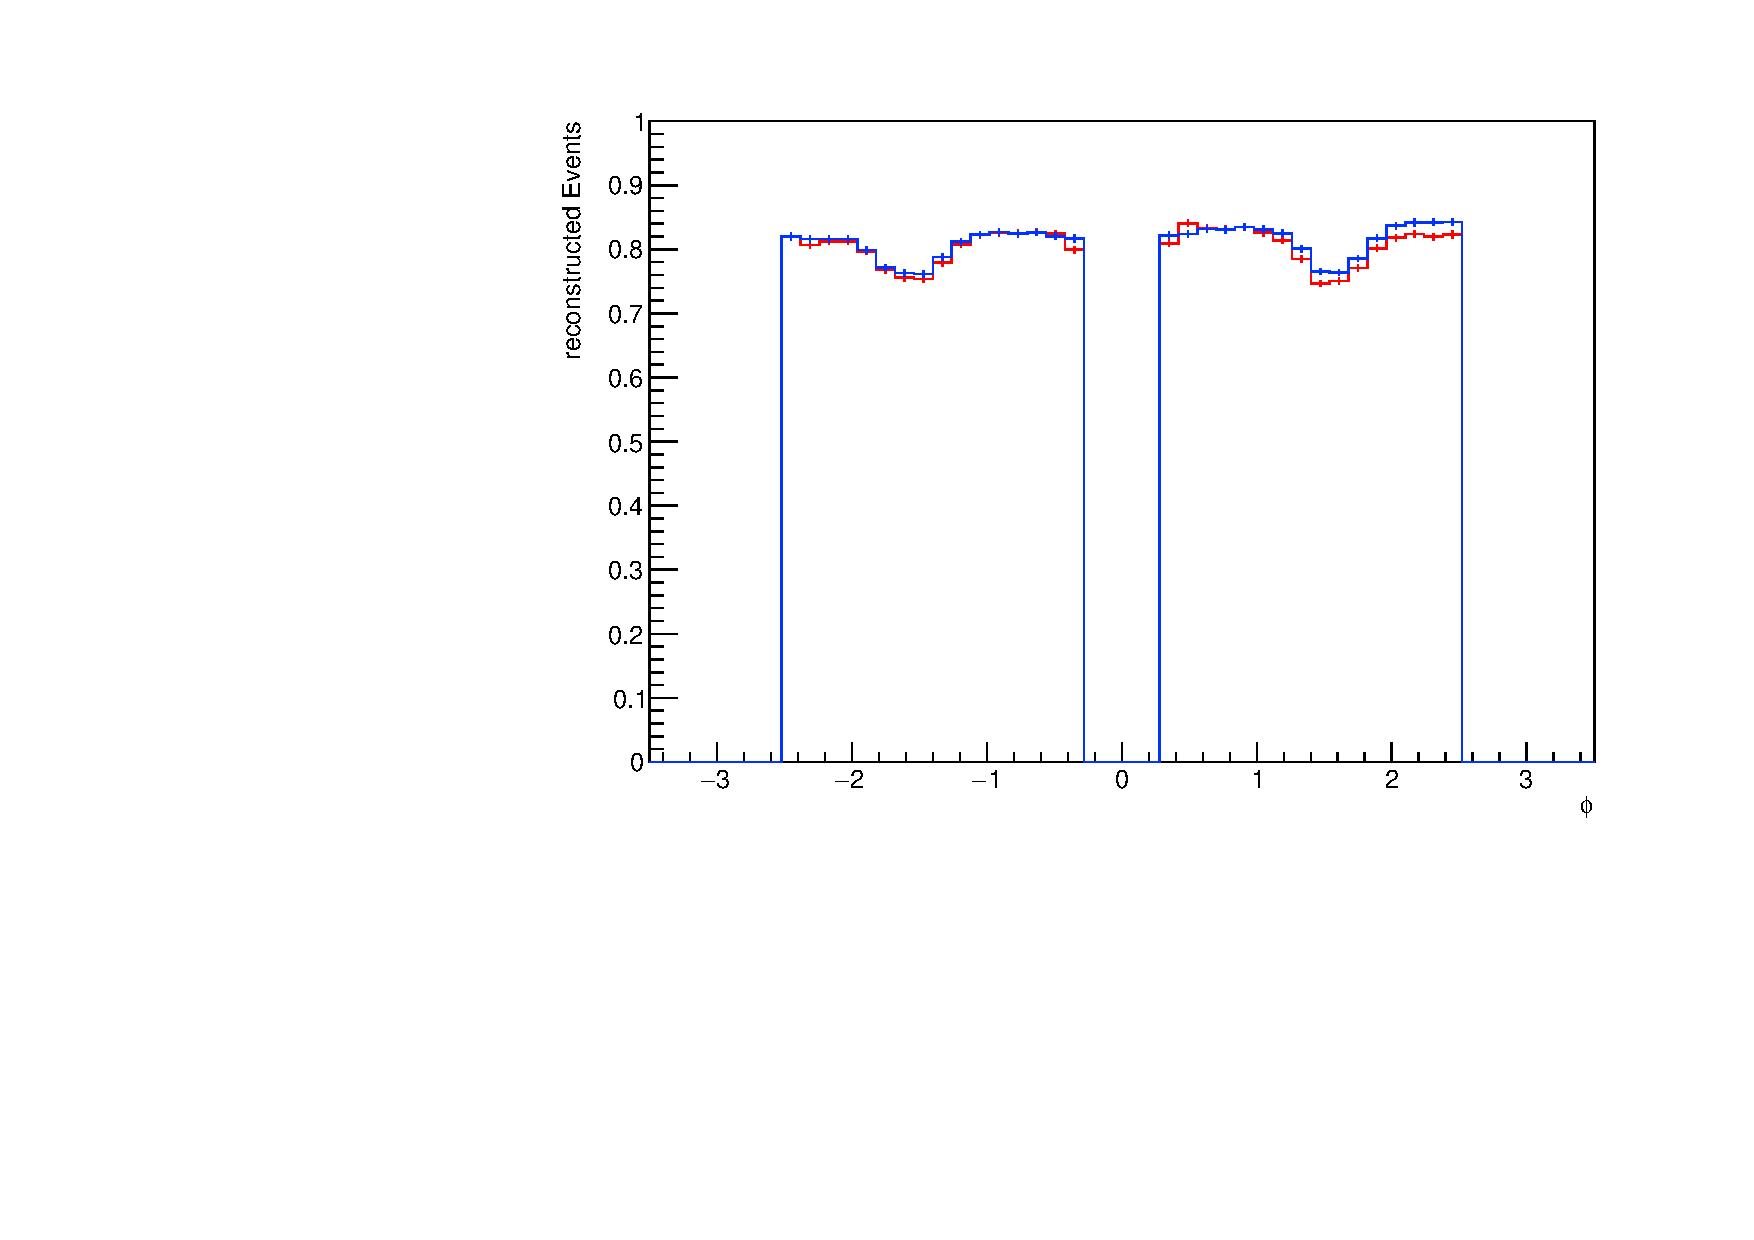
\includegraphics[width=0.9\textwidth]{sec/up_pdf/combined/h_phi_reco_SPi.pdf}
\end{subfigure}
\begin{subfigure}{0.45\textwidth}
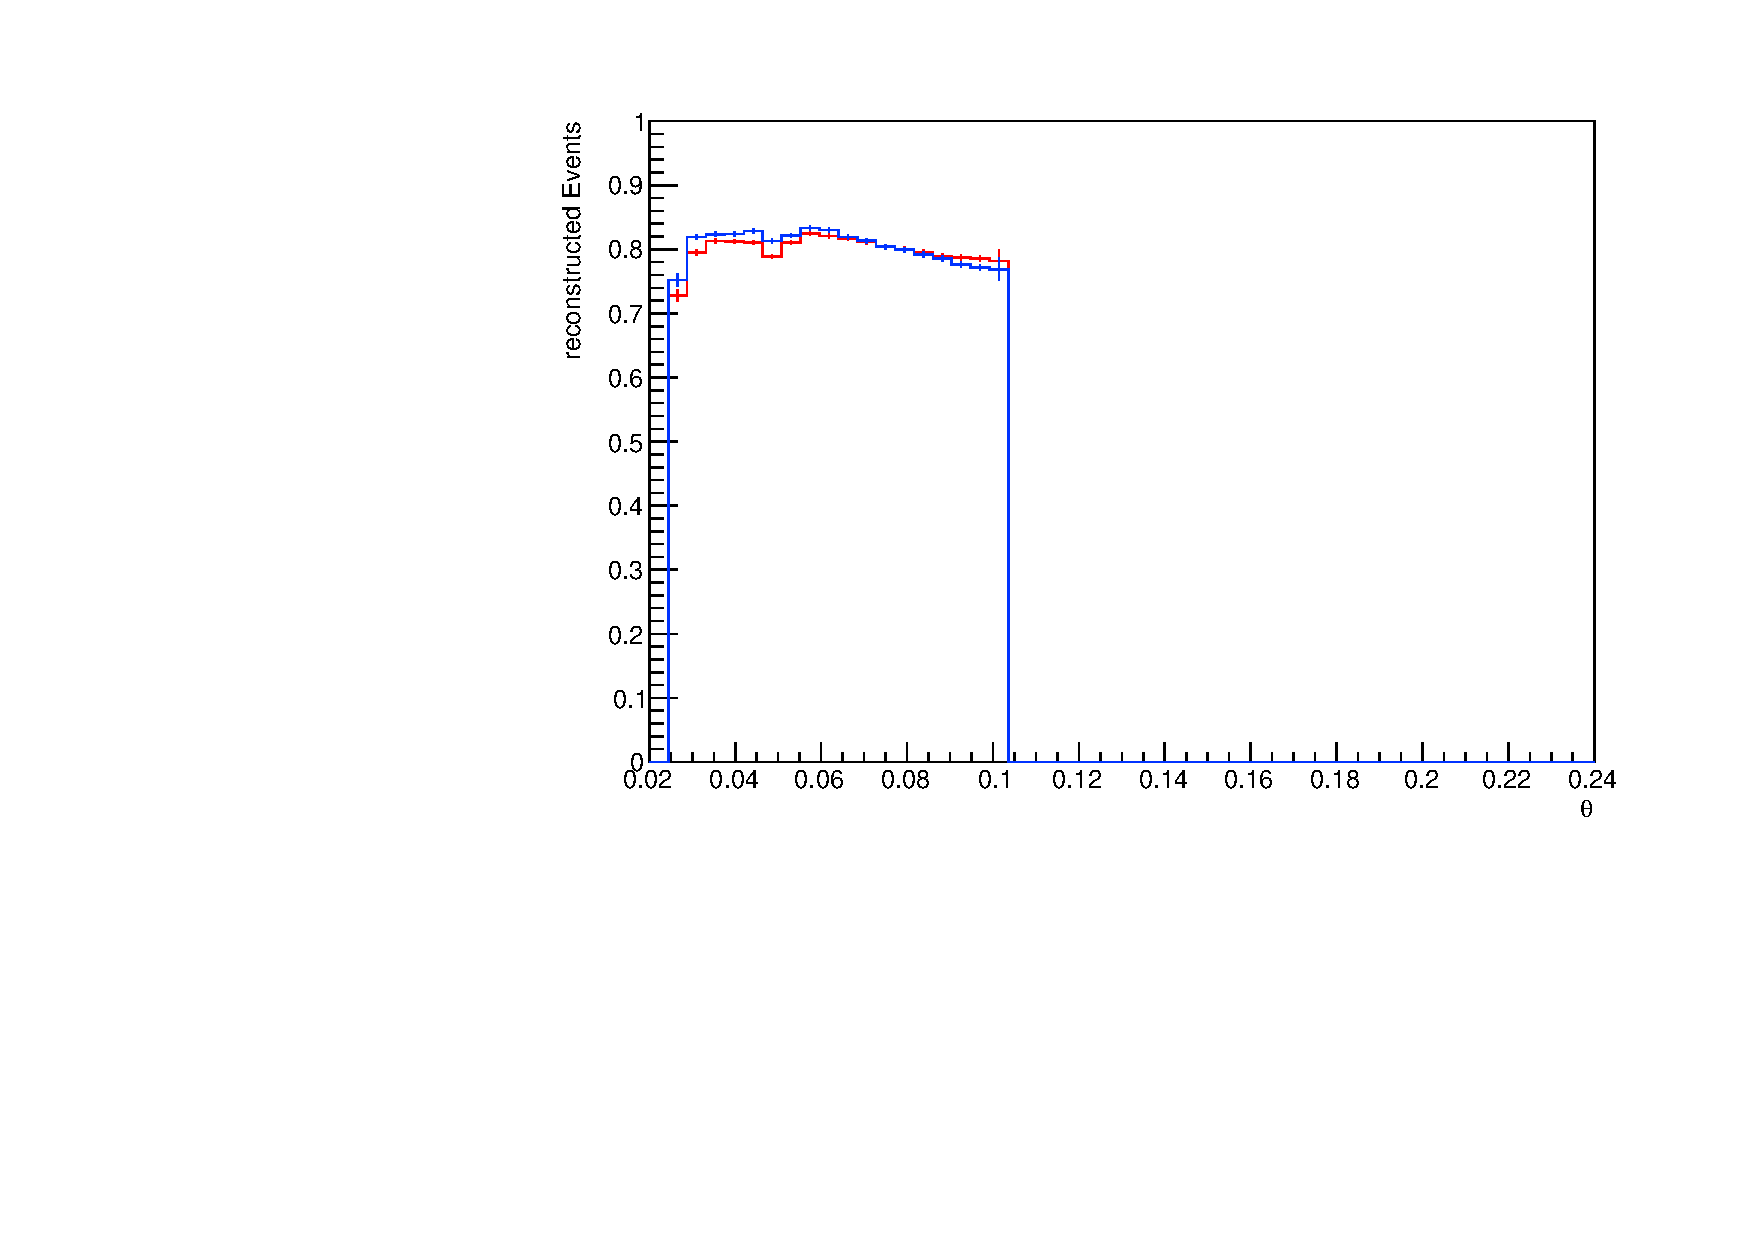
\includegraphics[width=0.9\textwidth]{sec/up_pdf/combined/h_theta_reco_SPi.pdf}
\end{subfigure}
\begin{subfigure}{0.45\textwidth}
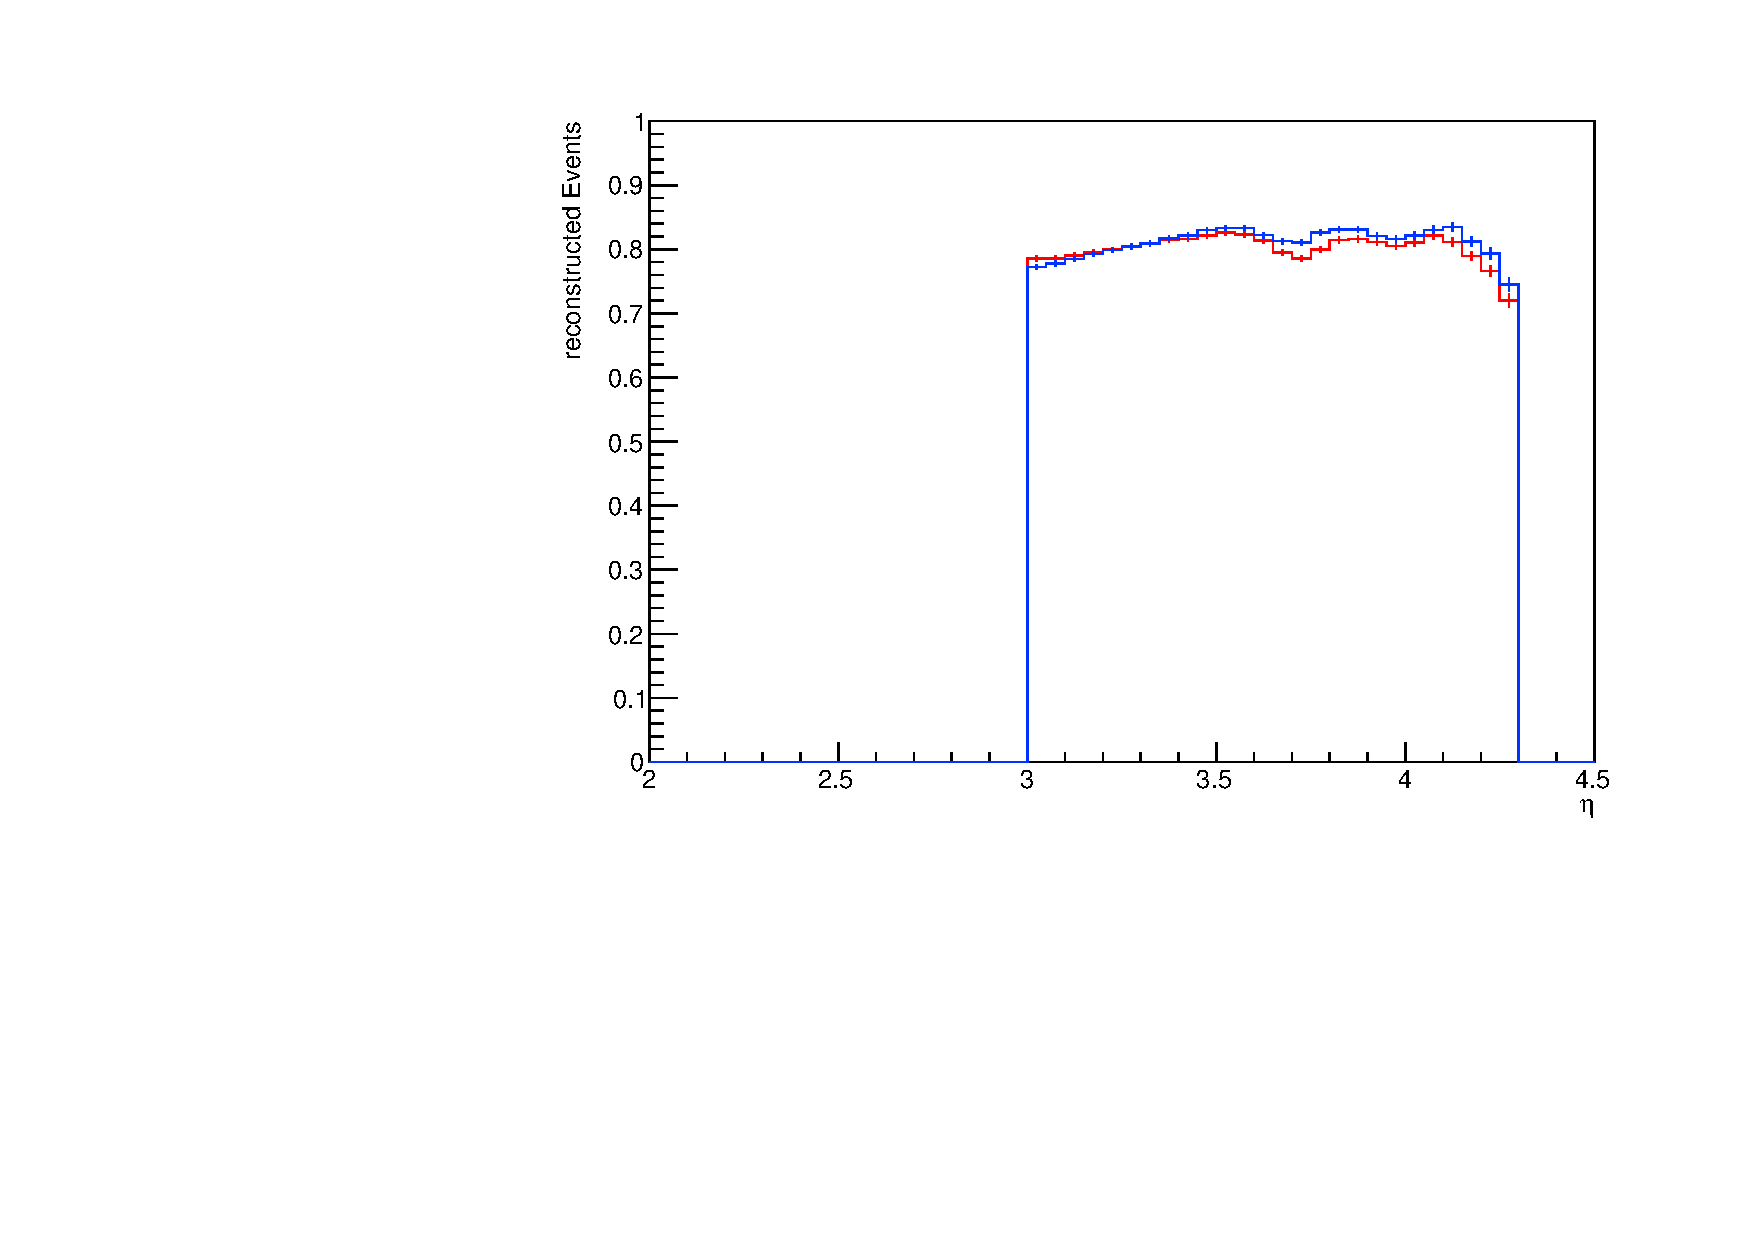
\includegraphics[width=0.9\textwidth]{sec/up_pdf/combined/h_eta_reco_SPi.pdf}
\end{subfigure}
\end{figure}
\end{frame}
\begin{frame}{Comparison of different charges with $DOWN$ polarity - soft $\pi$}
\begin{figure}
\begin{subfigure}{0.45\textwidth}
\includegraphics[width=0.9\textwidth]{sec/down_pdf/combined/h_pt_reco_SPi.pdf}
\end{subfigure}
\begin{subfigure}{0.45\textwidth}
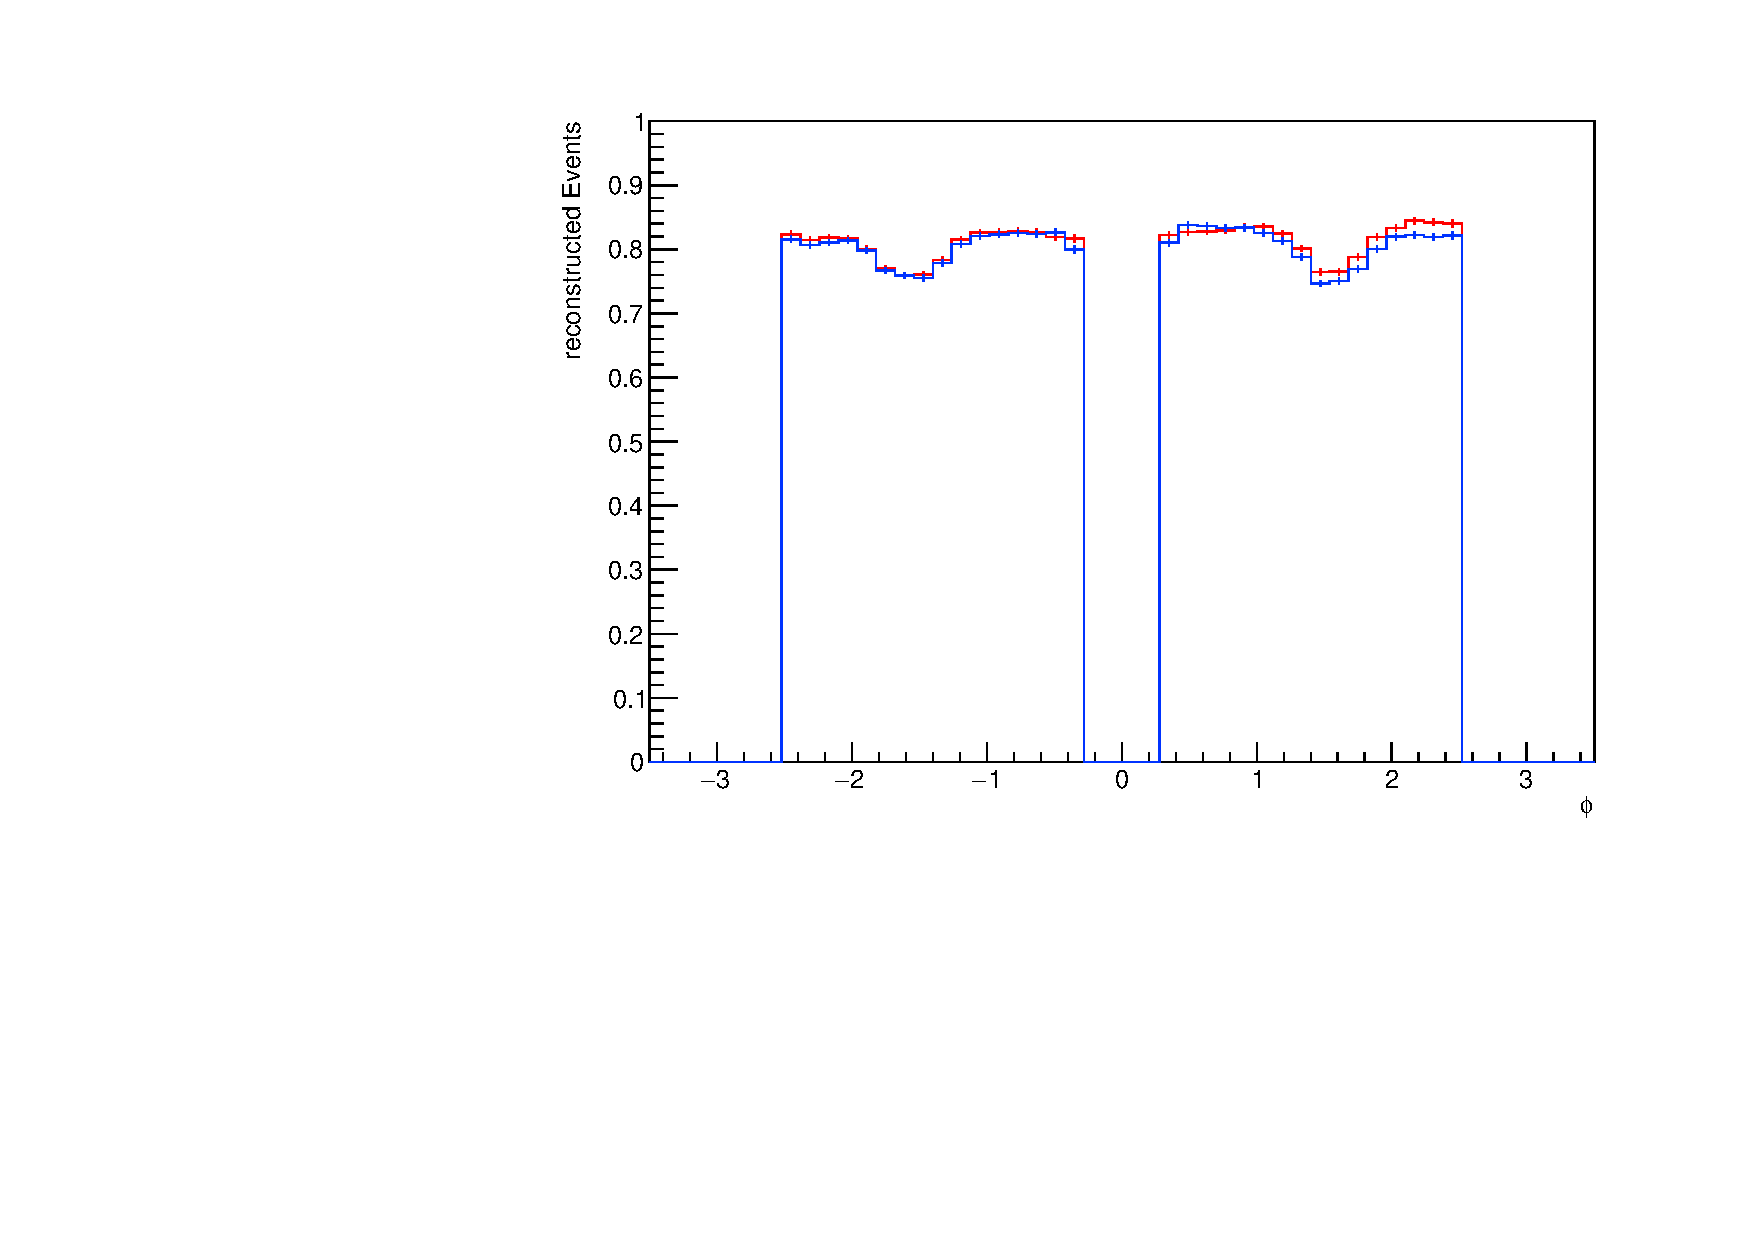
\includegraphics[width=0.9\textwidth]{sec/down_pdf/combined/h_phi_reco_SPi.pdf}
\end{subfigure}
\begin{subfigure}{0.45\textwidth}
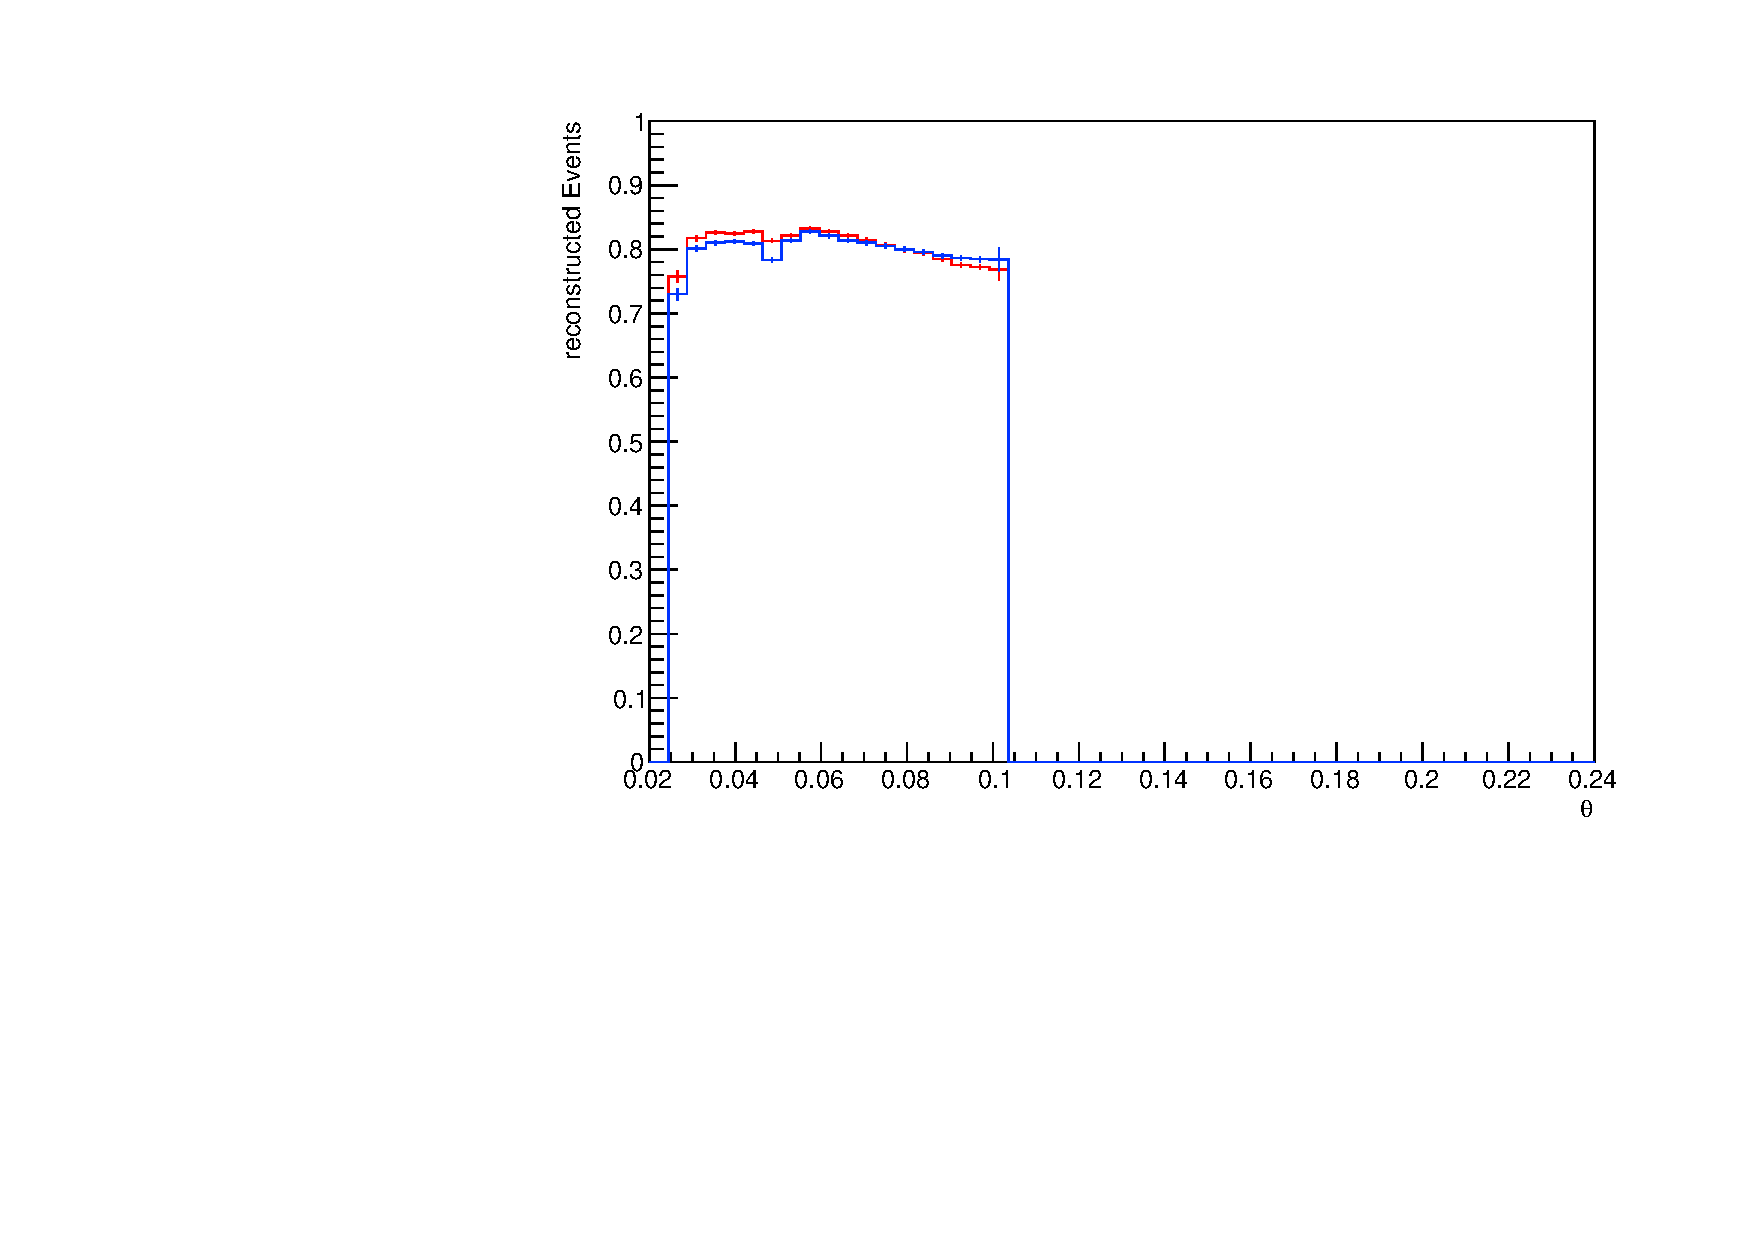
\includegraphics[width=0.9\textwidth]{sec/down_pdf/combined/h_theta_reco_SPi.pdf}
\end{subfigure}
\begin{subfigure}{0.45\textwidth}
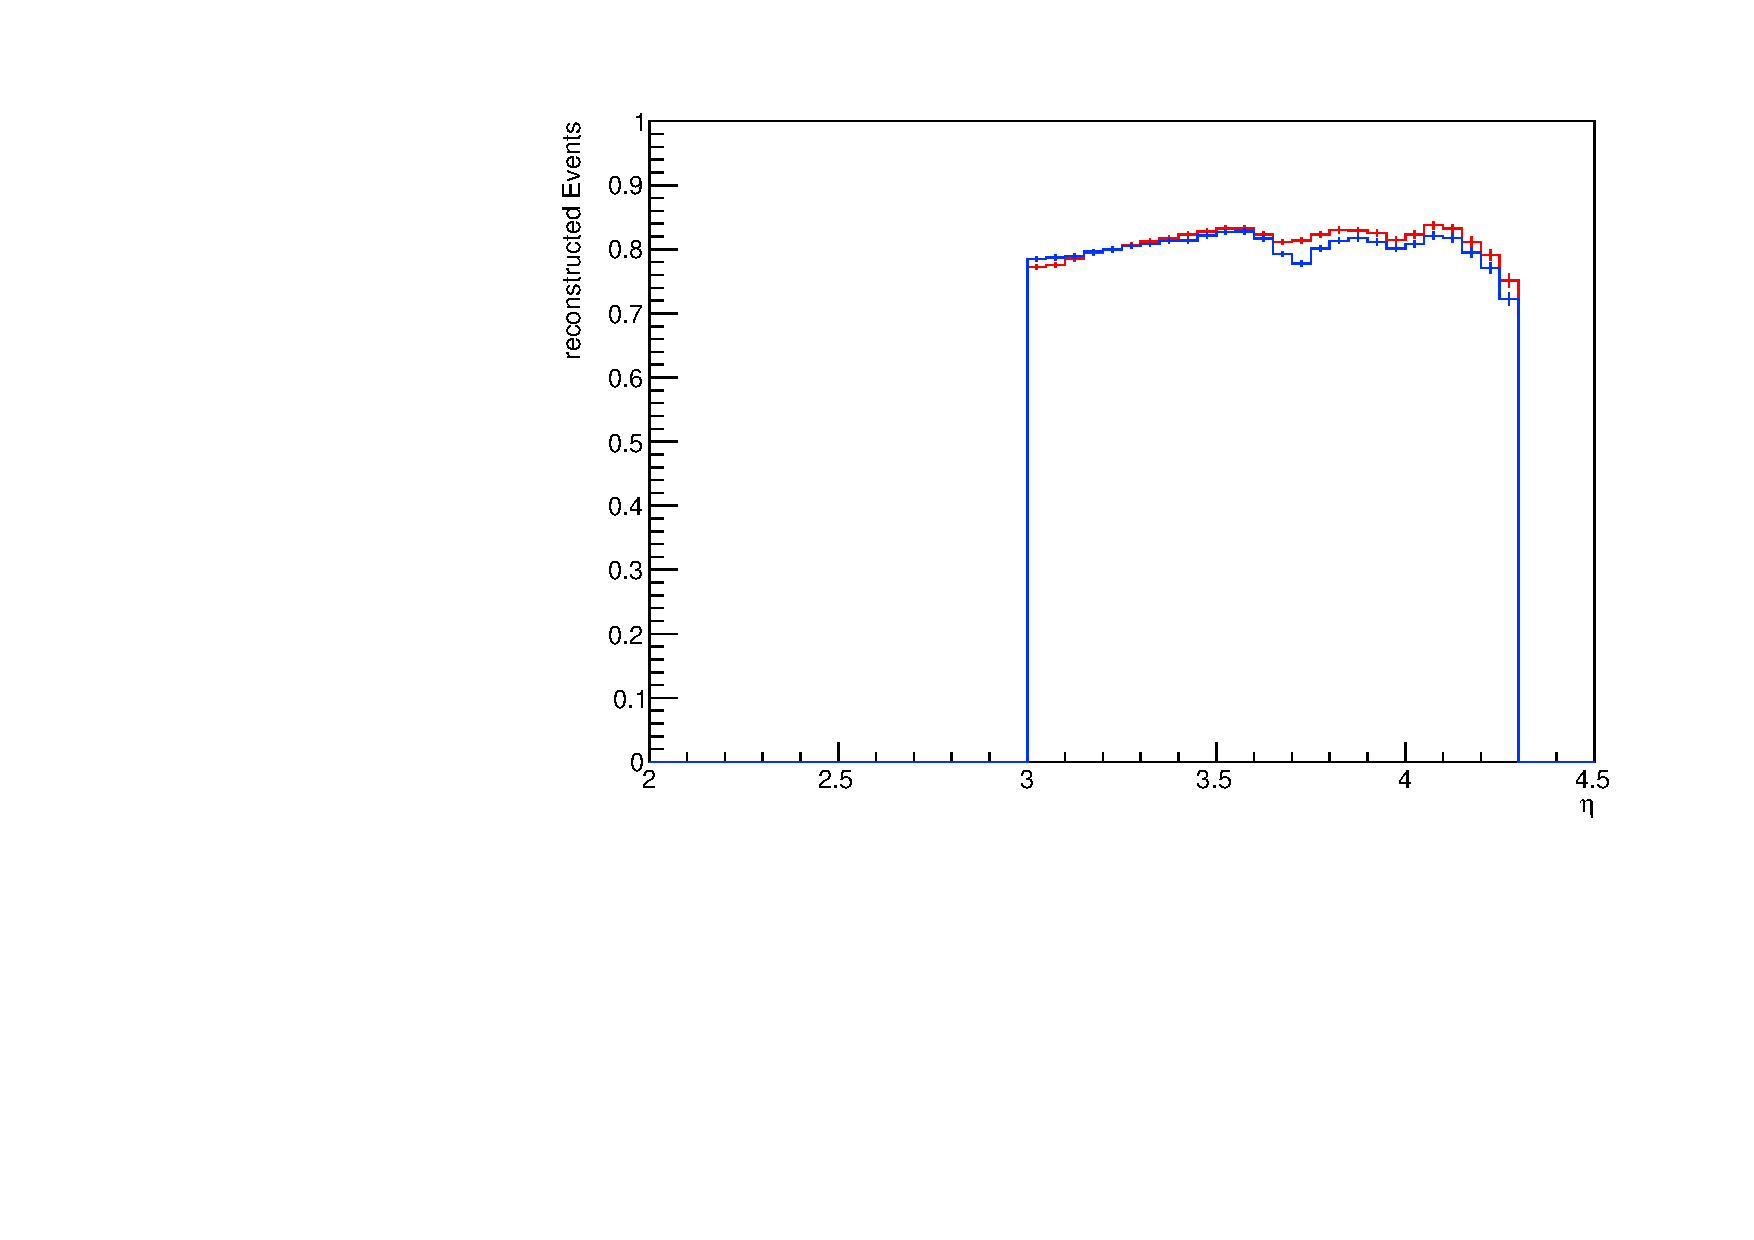
\includegraphics[width=0.9\textwidth]{sec/down_pdf/combined/h_eta_reco_SPi.pdf}
\end{subfigure}
\end{figure}
\end{frame}
\begin{frame}{Comparison - soft $\pi p_\text{T}$}
\centering
\includegraphics[width=0.48\textwidth]{sec/up_pdf/combined/h_pt_reco_SPi.pdf}
\includegraphics[width=0.48\textwidth]{sec/down_pdf/combined/h_pt_reco_SPi.pdf}
\end{frame}
\begin{frame}{Comparison - soft $\pi \phi$}
\centering
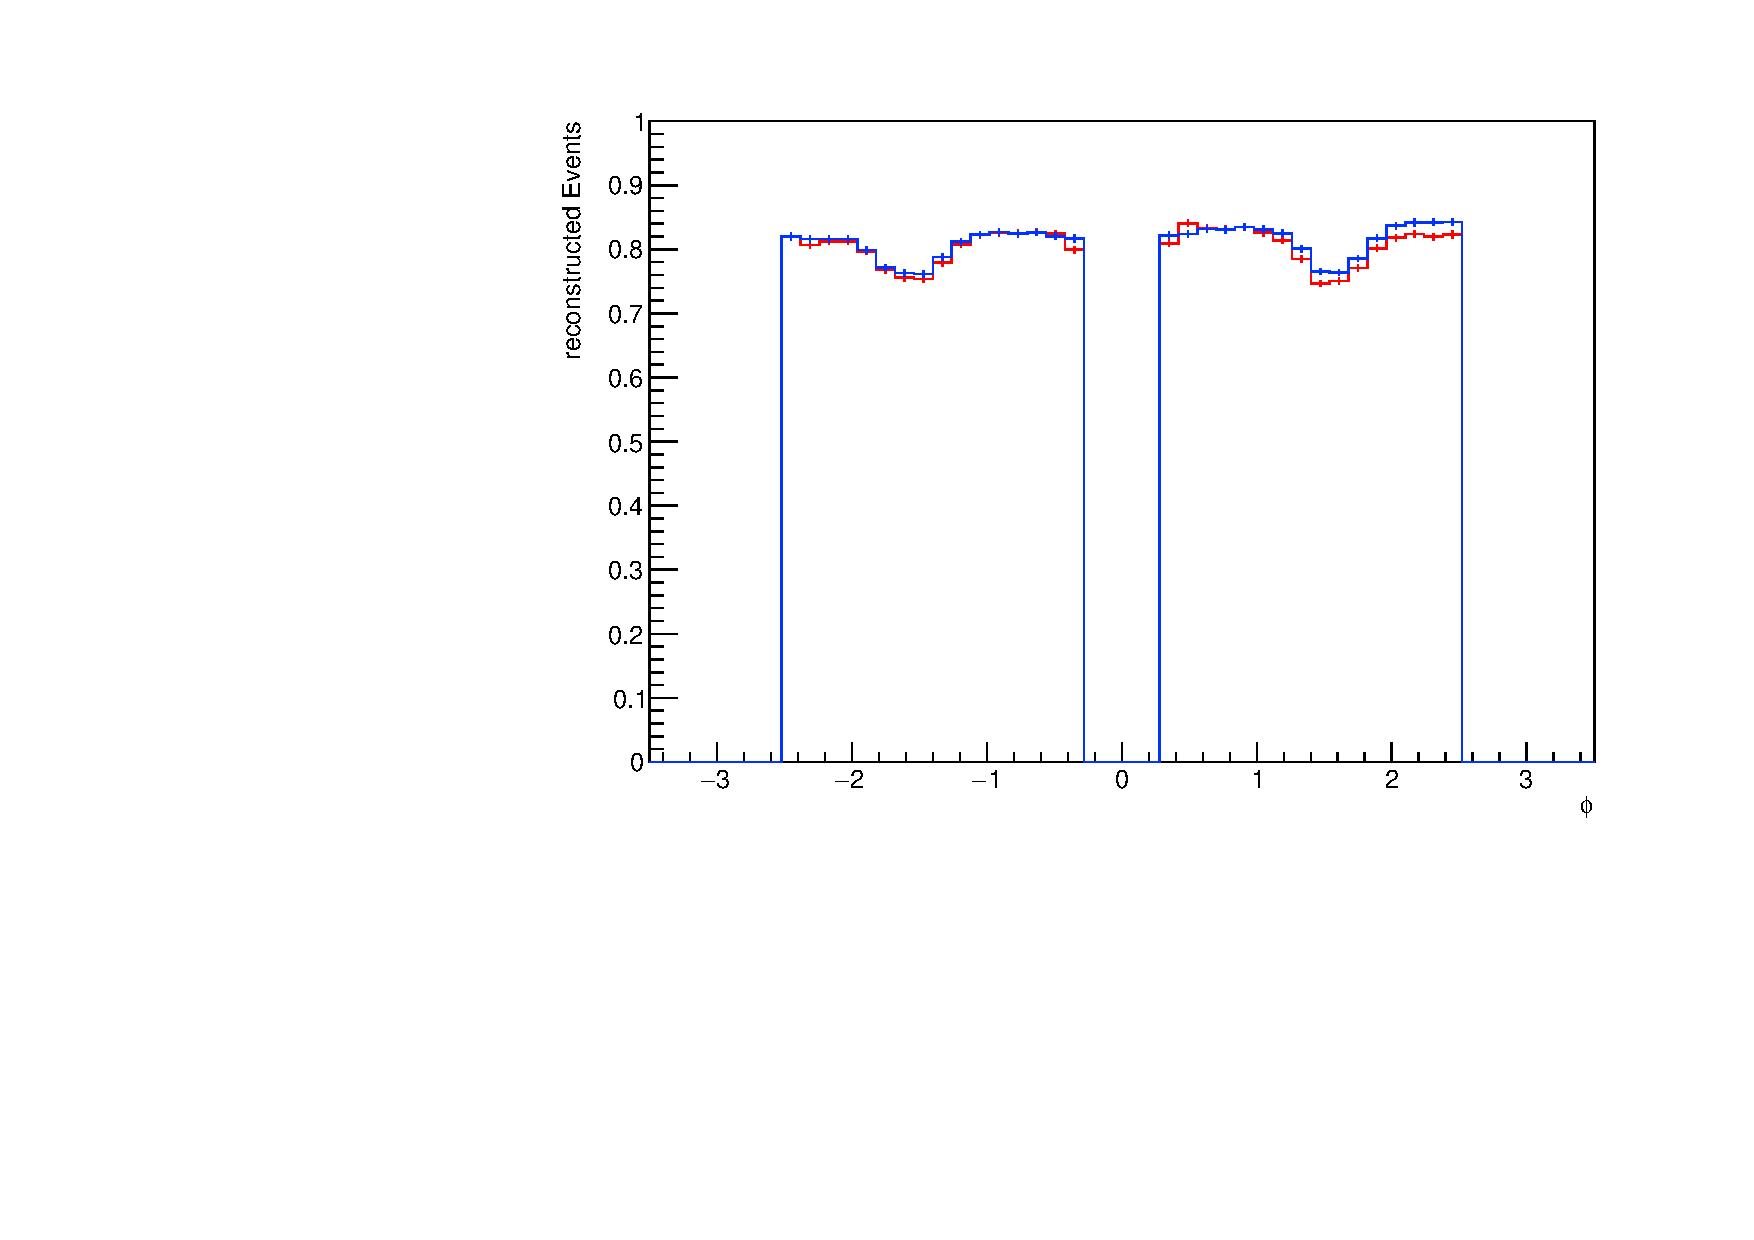
\includegraphics[width=0.48\textwidth]{sec/up_pdf/combined/h_phi_reco_SPi.pdf}
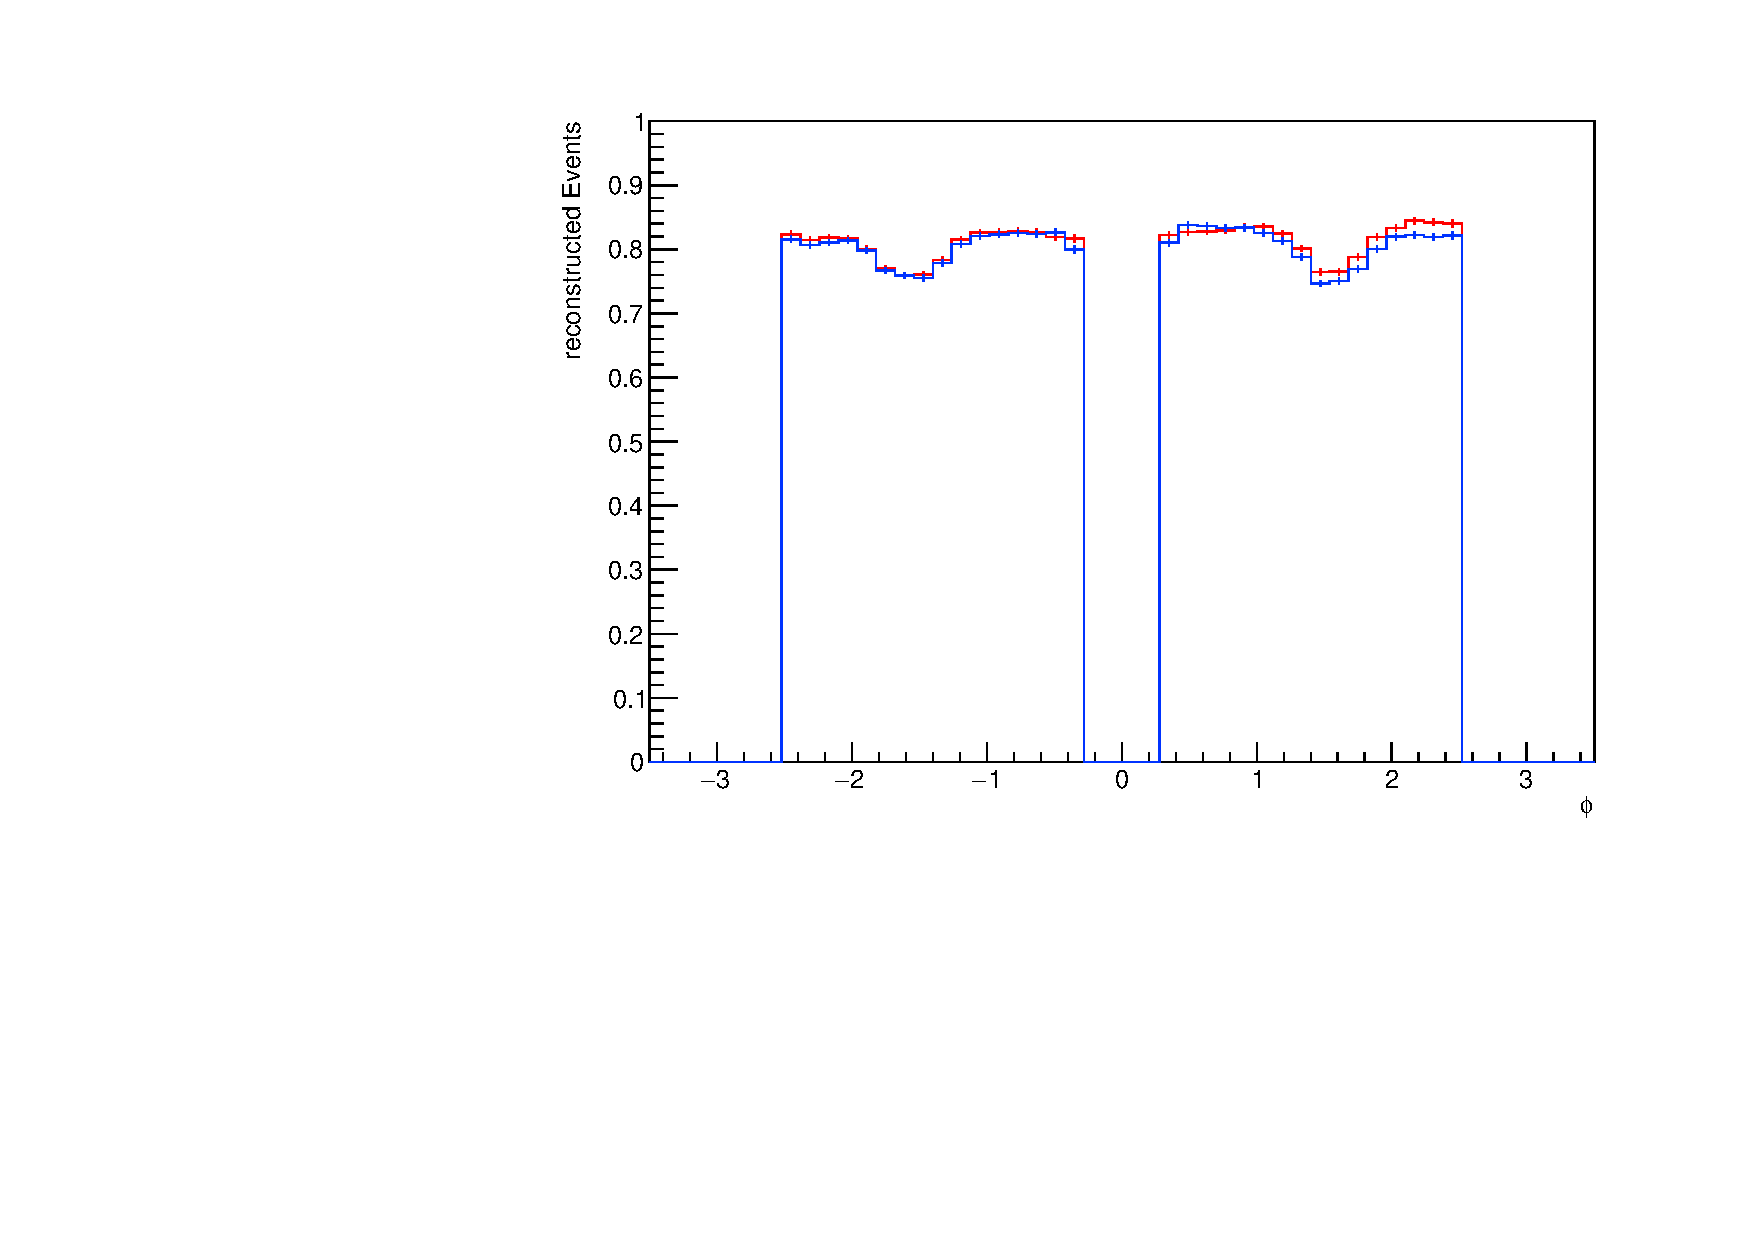
\includegraphics[width=0.48\textwidth]{sec/down_pdf/combined/h_phi_reco_SPi.pdf}
\end{frame}
\begin{frame}{Comparison - soft $\pi \theta$}
\centering
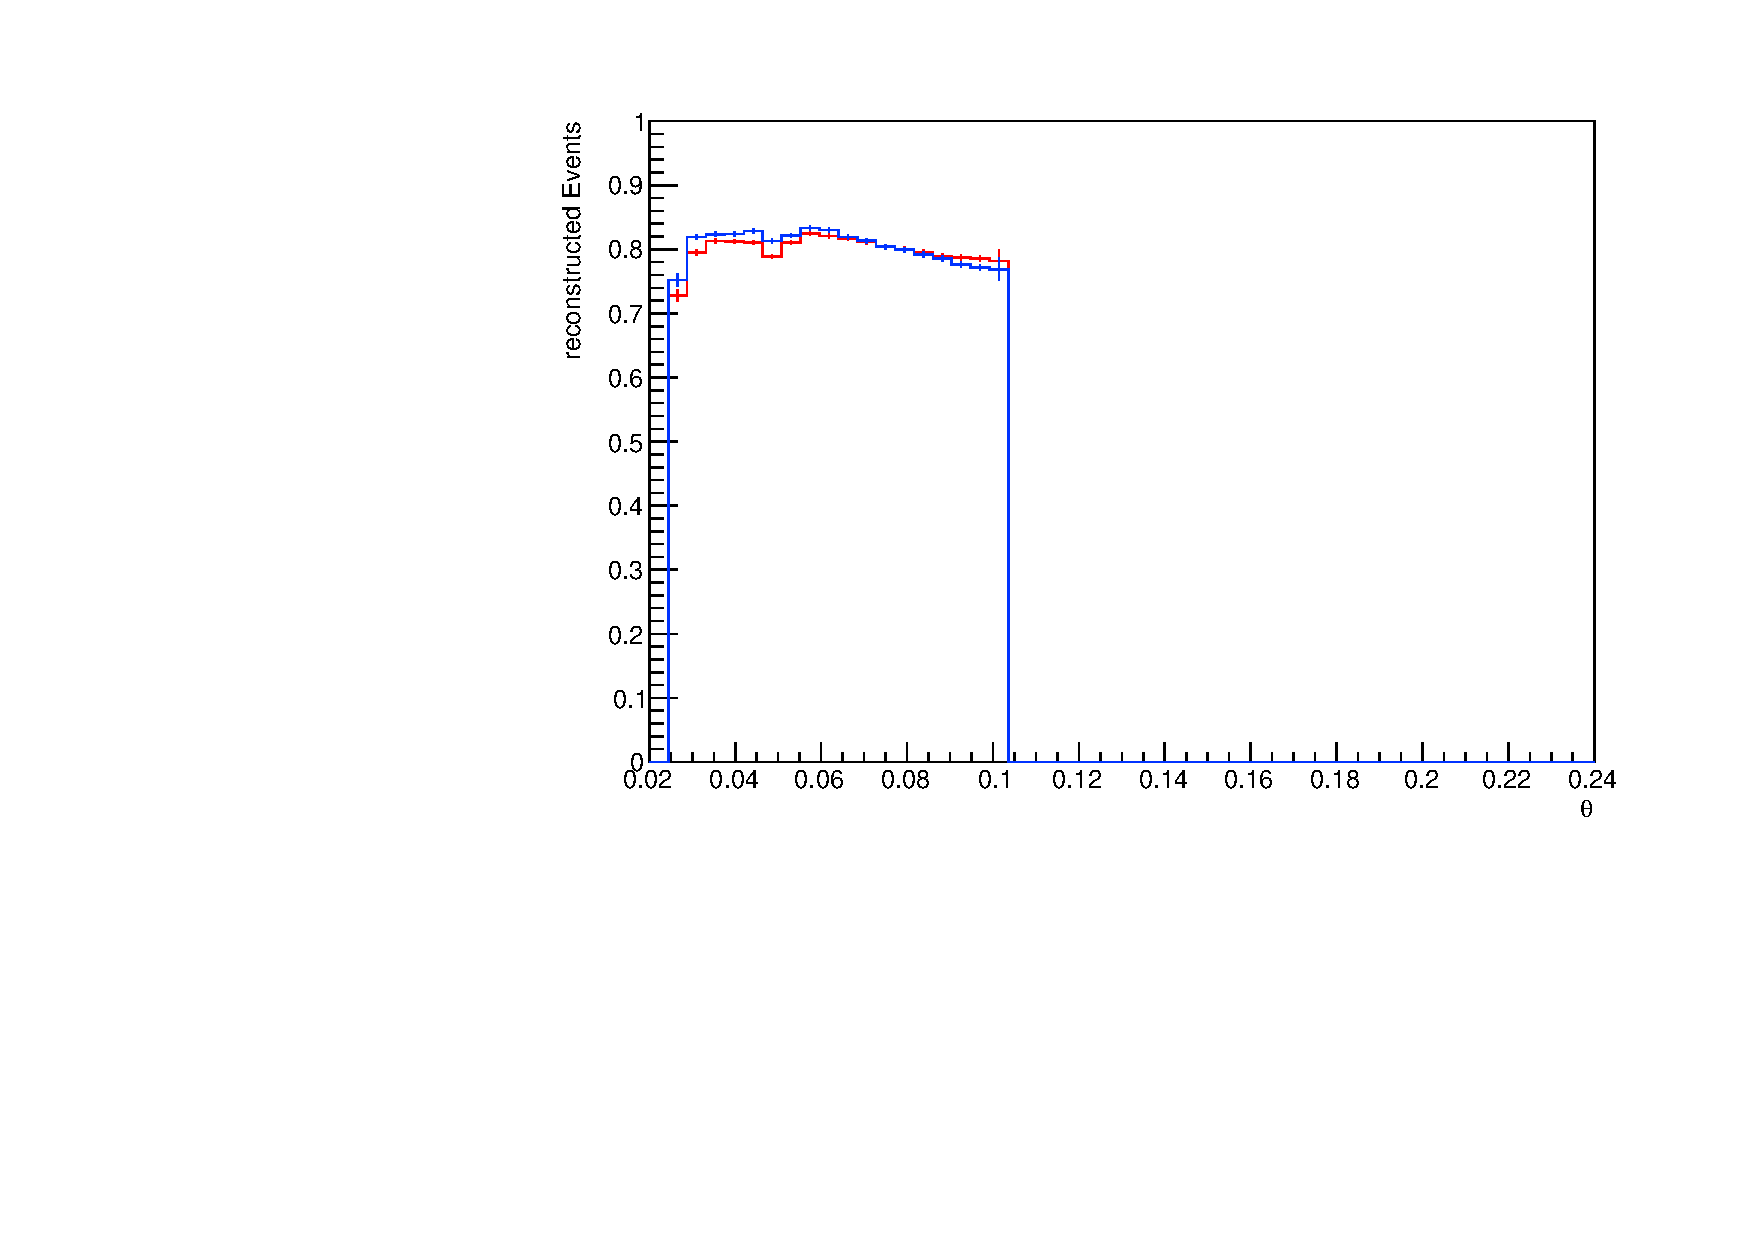
\includegraphics[width=0.48\textwidth]{sec/up_pdf/combined/h_theta_reco_SPi.pdf}
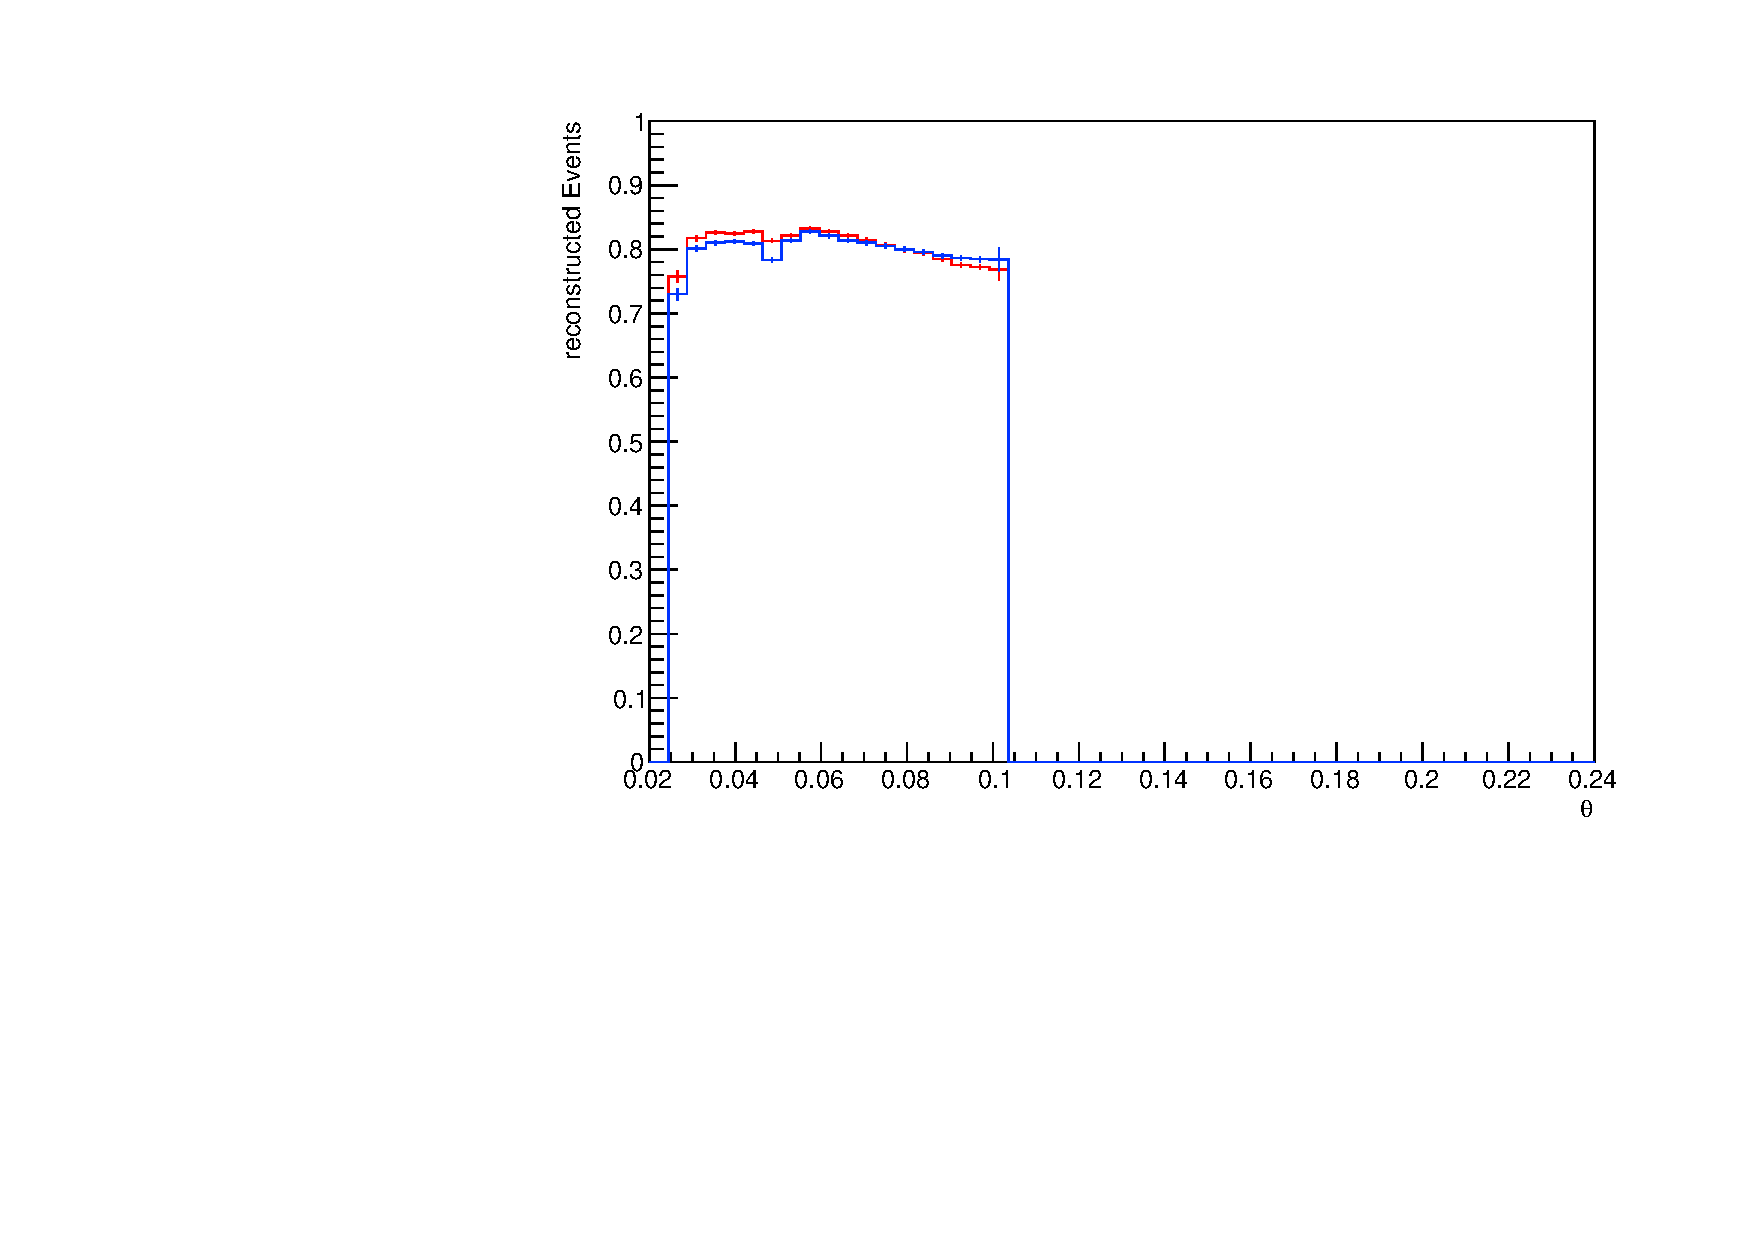
\includegraphics[width=0.48\textwidth]{sec/down_pdf/combined/h_theta_reco_SPi.pdf}
\end{frame}
\begin{frame}{Comparison - soft $\pi \eta$}
\centering
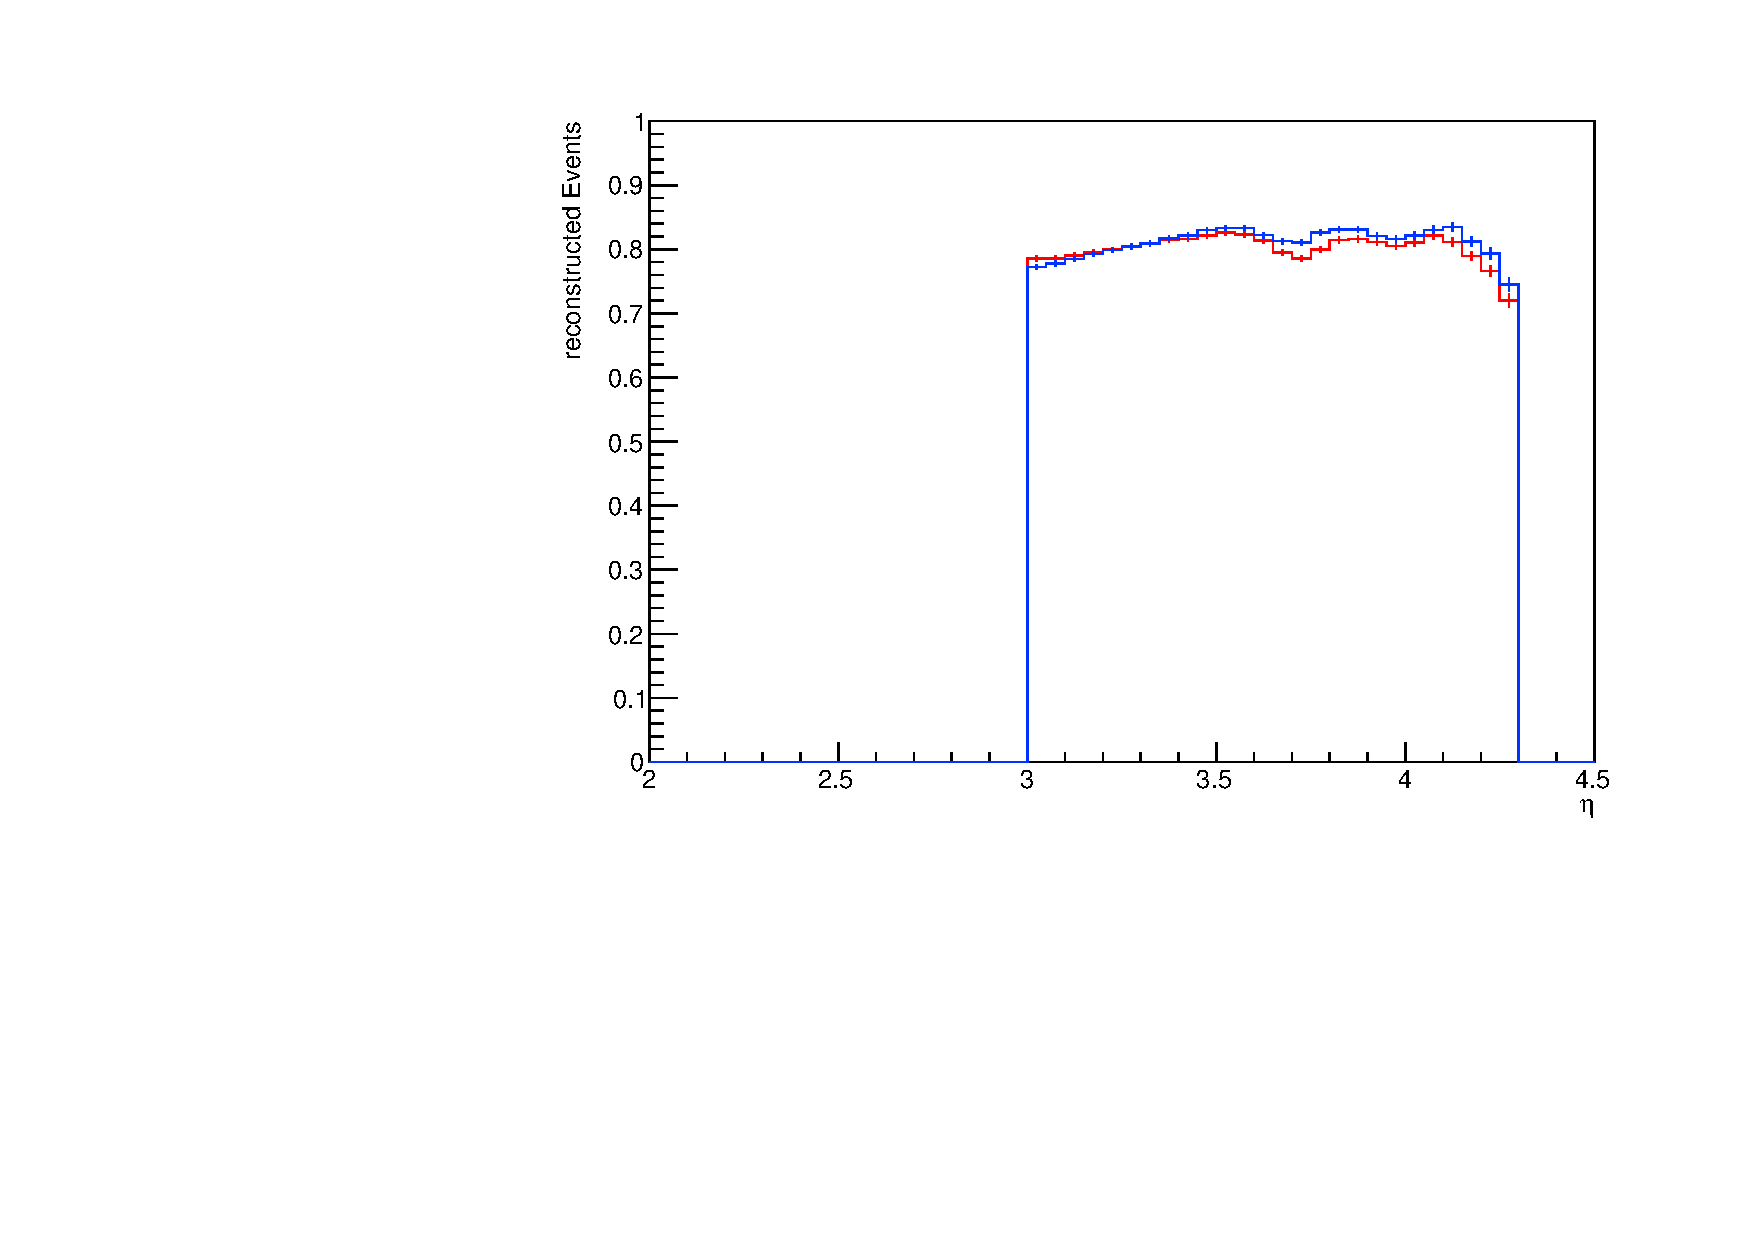
\includegraphics[width=0.48\textwidth]{sec/up_pdf/combined/h_eta_reco_SPi.pdf}
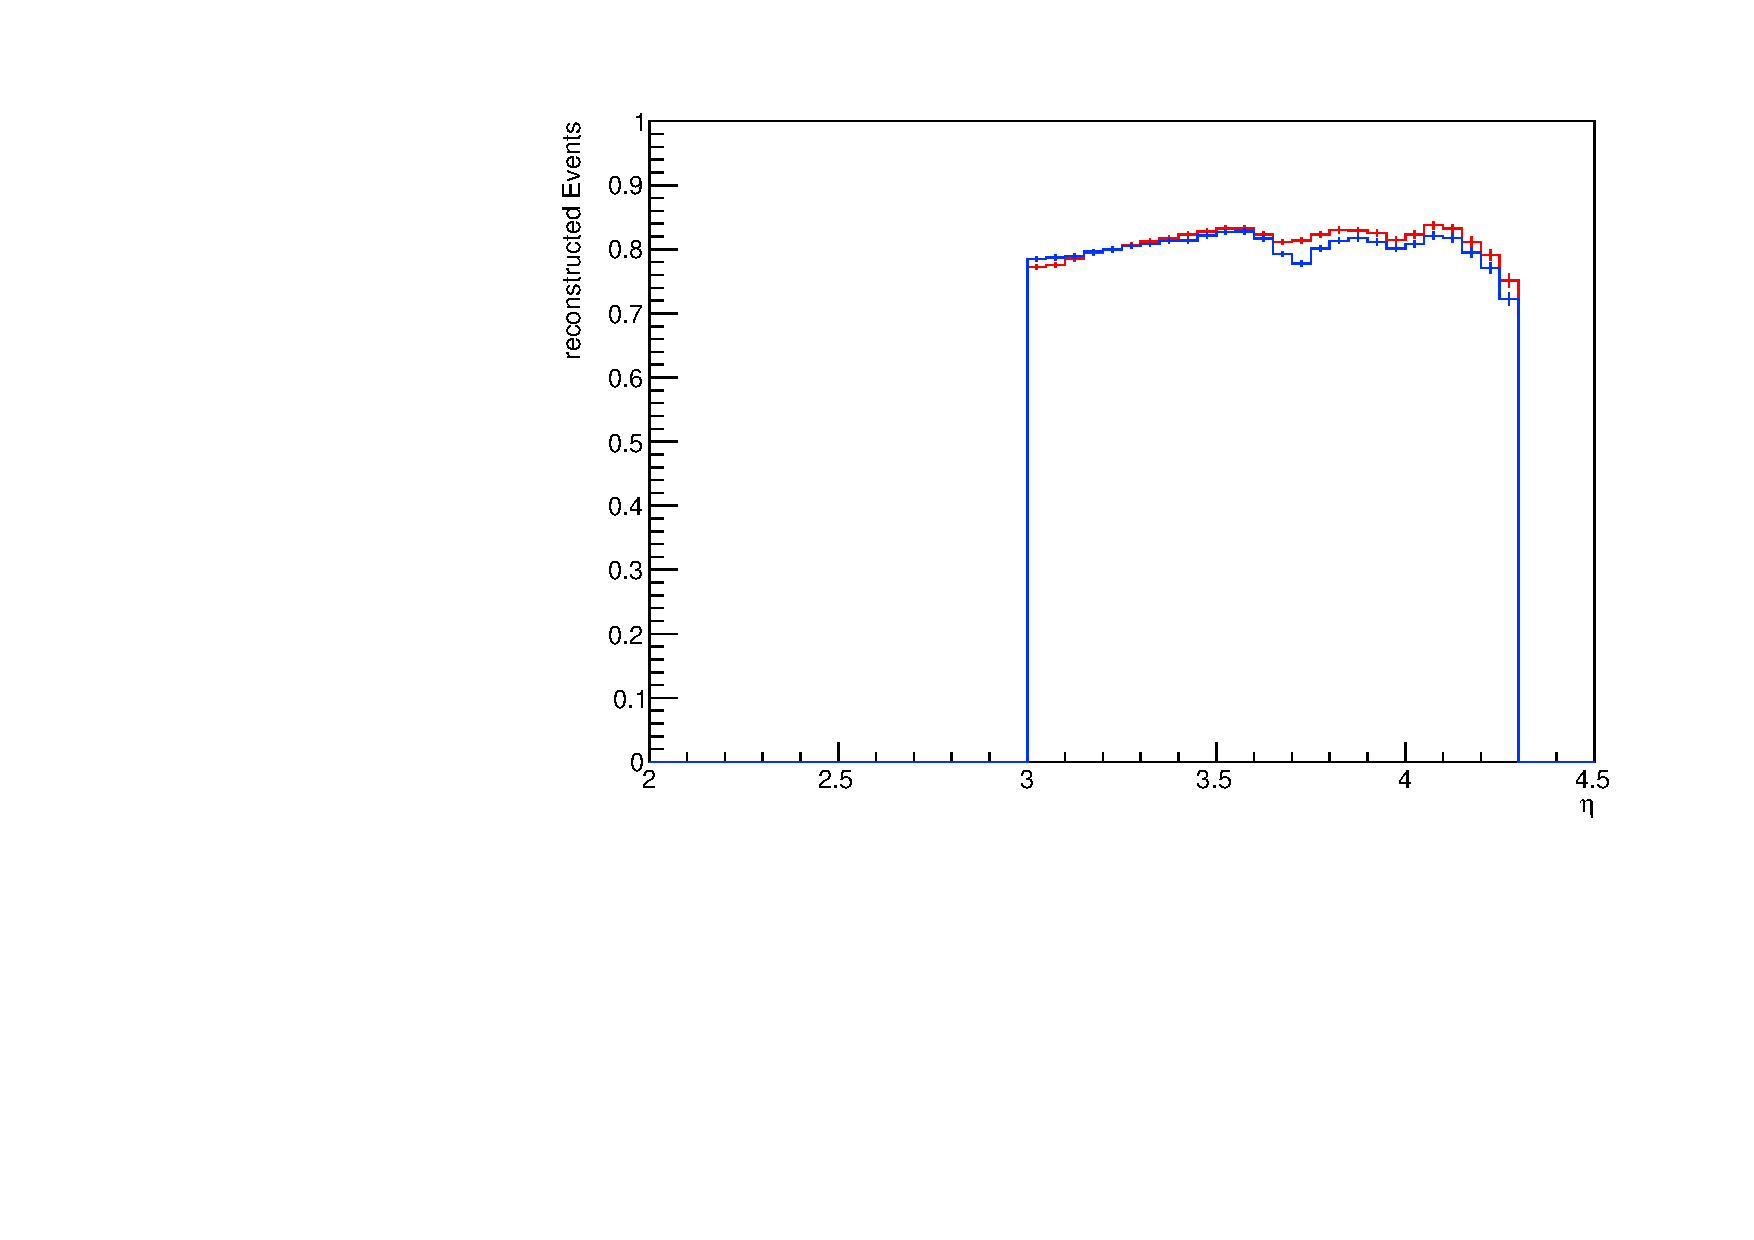
\includegraphics[width=0.48\textwidth]{sec/down_pdf/combined/h_eta_reco_SPi.pdf}
\end{frame}
\begin{frame}{soft $\pi$ deviation dependencies - $UP$ polarity}
\begin{figure}
\begin{subfigure}{0.45\textwidth}
\includegraphics[width=0.9\textwidth]{sec/up_pdf/deviation/h_pt_reco_SPi_pos_dev.pdf}
\end{subfigure}
\begin{subfigure}{0.45\textwidth}
\includegraphics[width=0.9\textwidth]{sec/up_pdf/deviation/h_phi_reco_SPi_pos_dev.pdf}
\end{subfigure}
\begin{subfigure}{0.45\textwidth}
\includegraphics[width=0.9\textwidth]{sec/up_pdf/deviation/h_theta_reco_SPi_pos_dev.pdf}
\end{subfigure}
\begin{subfigure}{0.45\textwidth}
\includegraphics[width=0.9\textwidth]{sec/up_pdf/deviation/h_eta_reco_SPi_pos_dev.pdf}
\end{subfigure}
\end{figure}
\end{frame}
\begin{frame}{soft $\pi$ deviation dependencies - $DOWN$ polarity}
\begin{figure}
\begin{subfigure}{0.45\textwidth}
\includegraphics[width=0.9\textwidth]{sec/down_pdf/deviation/h_pt_reco_SPi_pos_dev.pdf}
\end{subfigure}
\begin{subfigure}{0.45\textwidth}
\includegraphics[width=0.9\textwidth]{sec/down_pdf/deviation/h_phi_reco_SPi_pos_dev.pdf}
\end{subfigure}
\begin{subfigure}{0.45\textwidth}
\includegraphics[width=0.9\textwidth]{sec/down_pdf/deviation/h_theta_reco_SPi_pos_dev.pdf}
\end{subfigure}
\begin{subfigure}{0.45\textwidth}
\includegraphics[width=0.9\textwidth]{sec/down_pdf/deviation/h_eta_reco_SPi_pos_dev.pdf}
\end{subfigure}
\end{figure}
\end{frame}
\begin{frame}{soft $\pi$ deviation - $\phi$}
\centering
\includegraphics[width=0.48\textwidth]{sec/up_pdf/deviation/h_phi_reco_SPi_pos_dev.pdf}
\includegraphics[width=0.48\textwidth]{sec/down_pdf/deviation/h_phi_reco_SPi_pos_dev.pdf}
\end{frame}
\begin{frame}{soft $\pi$ deviation UP+DOWN}
\begin{figure}
\begin{subfigure}{0.45\textwidth}
\includegraphics[width=0.9\textwidth]{sec/up_plus_down_pdf/pT_2.pdf}
\end{subfigure}
\begin{subfigure}{0.45\textwidth}
\includegraphics[width=0.9\textwidth]{sec/up_plus_down_pdf/phi_2.pdf}
\end{subfigure}
\begin{subfigure}{0.45\textwidth}
\includegraphics[width=0.9\textwidth]{sec/up_plus_down_pdf/theta_2.pdf}
\end{subfigure}
\begin{subfigure}{0.45\textwidth}
\includegraphics[width=0.9\textwidth]{sec/up_plus_down_pdf/eta_2.pdf}
\end{subfigure}
\end{figure}
\end{frame}
\begin{frame}{Idea 3}
\begin{itemize}
\item $|\phi| < 0.3 \& |\phi| > 2.5$ \& $\theta < 0.13$
\end{itemize}
\begin{figure}
\begin{subfigure}{0.45\textwidth}
\includegraphics[width=0.9\textwidth]{first/up_pdf/test_u/h_phi_test_SPi_combined.pdf}
\end{subfigure}
\begin{subfigure}{0.45\textwidth}
\includegraphics[width=0.9\textwidth]{first/down_pdf/test_d/h_phi_test_SPi_combined.pdf}
\end{subfigure}
\end{figure}
\end{frame}
\begin{frame}{Deviation before \& after cut}
\begin{table}
	\caption{The deviation $\frac{N_+ - N_-}{N_+ + N_-}/10^{-3}$}
	\resizebox{\textwidth}{!}{
	\begin{tabular}{cS[table-format=1.1]@{${}\pm{}$}S[table-format=1.1]S[table-format=1.1]@{${}\pm{}$}S[table-format=1.1]S[table-format=1.1]@{${}\pm{}$}S[table-format=1.1]S[table-format=1.1]@{${}\pm{}$}S[table-format=1.1]S[table-format=1.1]@{${}\pm{}$}S[table-format=1.1]}
		\toprule
		{Polarity} & \multicolumn{2}{c}{$\pi $} & \multicolumn{2}{c}{$ K $} & \multicolumn{2}{c}{$ soft \pi $} & \multicolumn{2}{c}{$ D^0 $} & \multicolumn{2}{c}{$ D^* $} \\
		\midrule
		$UP$ & -0.1 & 0.4 & 4.7 & 0.4 & -3.8 & 0.5 & -4.7 & 0.5 & -8.2 & 0.5 \\
		$DOWN$ & -0.3 & 0.4 & 5.2 & 0.4 & 3.7 & 0.5 & -5.0 & 0.5 & -0.8 & 0.5\\
		\bottomrule
	\end{tabular}}
	\resizebox{\textwidth}{!}{
	\begin{tabular}{cS[table-format=1.1]@{${}\pm{}$}S[table-format=1.1]S[table-format=1.1]@{${}\pm{}$}S[table-format=1.1]S[table-format=1.1]@{${}\pm{}$}S[table-format=1.1]S[table-format=1.1]@{${}\pm{}$}S[table-format=1.1]S[table-format=1.1]@{${}\pm{}$}S[table-format=1.1]}
		\toprule
		{Polarity} & \multicolumn{2}{c}{$\pi $} & \multicolumn{2}{c}{$ K $} & \multicolumn{2}{c}{$ soft \pi $} & \multicolumn{2}{c}{$ D^0 $} & \multicolumn{2}{c}{$ D^* $} \\
		\midrule
		$UP$ & -0.1 & 0.4 & 4.7 & 0.4 & -1.0 & 0.6 & -4.7 & 0.5 & -5.2 & 0.6\\
		$DOWN$ & -0.3 & 0.4 & 5.2 & 0.4 & 0.3 & 0.6 & -5.0 & 0.5 & -4.0 & 0.6\\
		%$UP$ & -0.1 & 0.4 & 4.7 & 0.4 & 1.2 & 0.6 & -4.7 & 0.5 & -3.0 & 0.6\\
		%$DOWN$ & -0.3 & 0.4 & 5.2 & 0.4 & -1.7 & 0.6 & -5.0 & 0.5 & -6.2 & 0.6\\
		\bottomrule
	\end{tabular}}
\end{table}
\begin{itemize}
\item lower deviation in soft $\pi$, but polarities are affected differently
\item $\approx 33\%$ of events is rejected
\end{itemize}
\end{frame}
\begin{frame}{Comparison of different charges with $UP$ polarity - soft $\pi$}
\begin{figure}
\begin{subfigure}{0.45\textwidth}
\includegraphics[width=0.9\textwidth]{third/up_pdf/combined/h_pt_reco_SPi.pdf}
\end{subfigure}
\begin{subfigure}{0.45\textwidth}
\includegraphics[width=0.9\textwidth]{third/up_pdf/combined/h_phi_reco_SPi.pdf}
\end{subfigure}
\begin{subfigure}{0.45\textwidth}
\includegraphics[width=0.9\textwidth]{third/up_pdf/combined/h_theta_reco_SPi.pdf}
\end{subfigure}
\begin{subfigure}{0.45\textwidth}
\includegraphics[width=0.9\textwidth]{third/up_pdf/combined/h_eta_reco_SPi.pdf}
\end{subfigure}
\end{figure}
\end{frame}
\begin{frame}{Comparison of different charges with $DOWN$ polarity - soft $\pi$}
\begin{figure}
\begin{subfigure}{0.45\textwidth}
\includegraphics[width=0.9\textwidth]{third/down_pdf/combined/h_pt_reco_SPi.pdf}
\end{subfigure}
\begin{subfigure}{0.45\textwidth}
\includegraphics[width=0.9\textwidth]{third/down_pdf/combined/h_phi_reco_SPi.pdf}
\end{subfigure}
\begin{subfigure}{0.45\textwidth}
\includegraphics[width=0.9\textwidth]{third/down_pdf/combined/h_theta_reco_SPi.pdf}
\end{subfigure}
\begin{subfigure}{0.45\textwidth}
\includegraphics[width=0.9\textwidth]{third/down_pdf/combined/h_eta_reco_SPi.pdf}
\end{subfigure}
\end{figure}
\end{frame}
\begin{frame}{Comparison - soft $\pi p_\text{T}$}
\centering
\includegraphics[width=0.48\textwidth]{third/up_pdf/combined/h_pt_reco_SPi.pdf}
\includegraphics[width=0.48\textwidth]{third/down_pdf/combined/h_pt_reco_SPi.pdf}
\end{frame}
\begin{frame}{Comparison - soft $\pi \phi$}
\centering
\includegraphics[width=0.48\textwidth]{third/up_pdf/combined/h_phi_reco_SPi.pdf}
\includegraphics[width=0.48\textwidth]{third/down_pdf/combined/h_phi_reco_SPi.pdf}
\end{frame}
\begin{frame}{Comparison - soft $\pi \theta$}
\centering
\includegraphics[width=0.48\textwidth]{third/up_pdf/combined/h_theta_reco_SPi.pdf}
\includegraphics[width=0.48\textwidth]{third/down_pdf/combined/h_theta_reco_SPi.pdf}
\end{frame}
\begin{frame}{Comparison - soft $\pi \eta$}
\centering
\includegraphics[width=0.48\textwidth]{third/up_pdf/combined/h_eta_reco_SPi.pdf}
\includegraphics[width=0.48\textwidth]{third/down_pdf/combined/h_eta_reco_SPi.pdf}
\end{frame}
\begin{frame}{soft $\pi$ deviation dependencies - $UP$ polarity}
\begin{figure}
\begin{subfigure}{0.45\textwidth}
\includegraphics[width=0.9\textwidth]{third/up_pdf/deviation/h_pt_reco_SPi_pos_dev.pdf}
\end{subfigure}
\begin{subfigure}{0.45\textwidth}
\includegraphics[width=0.9\textwidth]{third/up_pdf/deviation/h_phi_reco_SPi_pos_dev.pdf}
\end{subfigure}
\begin{subfigure}{0.45\textwidth}
\includegraphics[width=0.9\textwidth]{third/up_pdf/deviation/h_theta_reco_SPi_pos_dev.pdf}
\end{subfigure}
\begin{subfigure}{0.45\textwidth}
\includegraphics[width=0.9\textwidth]{third/up_pdf/deviation/h_eta_reco_SPi_pos_dev.pdf}
\end{subfigure}
\end{figure}
\end{frame}
\begin{frame}{soft $\pi$ deviation dependencies - $DOWN$ polarity}
\begin{figure}
\begin{subfigure}{0.45\textwidth}
\includegraphics[width=0.9\textwidth]{third/down_pdf/deviation/h_pt_reco_SPi_pos_dev.pdf}
\end{subfigure}
\begin{subfigure}{0.45\textwidth}
\includegraphics[width=0.9\textwidth]{third/down_pdf/deviation/h_phi_reco_SPi_pos_dev.pdf}
\end{subfigure}
\begin{subfigure}{0.45\textwidth}
\includegraphics[width=0.9\textwidth]{third/down_pdf/deviation/h_theta_reco_SPi_pos_dev.pdf}
\end{subfigure}
\begin{subfigure}{0.45\textwidth}
\includegraphics[width=0.9\textwidth]{third/down_pdf/deviation/h_eta_reco_SPi_pos_dev.pdf}
\end{subfigure}
\end{figure}
\end{frame}
\begin{frame}{soft $\pi$ deviation - $\phi$}
\centering
\includegraphics[width=0.48\textwidth]{third/up_pdf/deviation/h_phi_reco_SPi_pos_dev.pdf}
\includegraphics[width=0.48\textwidth]{third/down_pdf/deviation/h_phi_reco_SPi_pos_dev.pdf}
\end{frame}
\begin{frame}{soft $\pi$ deviation UP+DOWN}
\begin{figure}
\begin{subfigure}{0.45\textwidth}
\includegraphics[width=0.9\textwidth]{third/up_plus_down_pdf/pT_2.pdf}
\end{subfigure}
\begin{subfigure}{0.45\textwidth}
\includegraphics[width=0.9\textwidth]{third/up_plus_down_pdf/phi_2.pdf}
\end{subfigure}
\begin{subfigure}{0.45\textwidth}
\includegraphics[width=0.9\textwidth]{third/up_plus_down_pdf/theta_2.pdf}
\end{subfigure}
\begin{subfigure}{0.45\textwidth}
\includegraphics[width=0.9\textwidth]{third/up_plus_down_pdf/eta_2.pdf}
\end{subfigure}
\end{figure}
\end{frame}
\begin{frame}{Idea 4}
\begin{itemize}
\item $|\phi| < 0.5 \& |\phi| > 2.5$ \& $\theta < 0.13$
\end{itemize}
\begin{figure}
\begin{subfigure}{0.45\textwidth}
\includegraphics[width=0.9\textwidth]{first/up_pdf/test_u/h_phi_test_SPi_combined.pdf}
\end{subfigure}
\begin{subfigure}{0.45\textwidth}
\includegraphics[width=0.9\textwidth]{first/down_pdf/test_d/h_phi_test_SPi_combined.pdf}
\end{subfigure}
\end{figure}
\end{frame}
\begin{frame}{Deviation before \& after cut}
\begin{table}
	\caption{The deviation $\frac{N_+ - N_-}{N_+ + N_-}/10^{-3}$}
	\resizebox{\textwidth}{!}{
	\begin{tabular}{cS[table-format=1.1]@{${}\pm{}$}S[table-format=1.1]S[table-format=1.1]@{${}\pm{}$}S[table-format=1.1]S[table-format=1.1]@{${}\pm{}$}S[table-format=1.1]S[table-format=1.1]@{${}\pm{}$}S[table-format=1.1]S[table-format=1.1]@{${}\pm{}$}S[table-format=1.1]}
		\toprule
		{Polarity} & \multicolumn{2}{c}{$\pi $} & \multicolumn{2}{c}{$ K $} & \multicolumn{2}{c}{$ soft \pi $} & \multicolumn{2}{c}{$ D^0 $} & \multicolumn{2}{c}{$ D^* $} \\
		\midrule
		$UP$ & -0.1 & 0.4 & 4.7 & 0.4 & -3.8 & 0.5 & -4.7 & 0.5 & -8.2 & 0.5 \\
		$DOWN$ & -0.3 & 0.4 & 5.2 & 0.4 & 3.7 & 0.5 & -5.0 & 0.5 & -0.8 & 0.5\\
		\bottomrule
	\end{tabular}}
	\resizebox{\textwidth}{!}{
	\begin{tabular}{cS[table-format=1.1]@{${}\pm{}$}S[table-format=1.1]S[table-format=1.1]@{${}\pm{}$}S[table-format=1.1]S[table-format=1.1]@{${}\pm{}$}S[table-format=1.1]S[table-format=1.1]@{${}\pm{}$}S[table-format=1.1]S[table-format=1.1]@{${}\pm{}$}S[table-format=1.1]}
		\toprule
		{Polarity} & \multicolumn{2}{c}{$\pi $} & \multicolumn{2}{c}{$ K $} & \multicolumn{2}{c}{$ soft \pi $} & \multicolumn{2}{c}{$ D^0 $} & \multicolumn{2}{c}{$ D^* $} \\
		\midrule
		$UP$ & -0.1 & 0.4 & 4.7 & 0.4 & -1.0 & 0.6 & -4.7 & 0.5 & -5.2 & 0.6\\
		$DOWN$ & -0.3 & 0.4 & 5.2 & 0.4 & 0.3 & 0.6 & -5.0 & 0.5 & -4.0 & 0.6\\
		\bottomrule
	\end{tabular}}
\end{table}
\begin{itemize}
\item lower deviation in soft $\pi$, but polarities are affected differently
\item $\approx 33\%$ of events is rejected
\end{itemize}
\end{frame}
\begin{frame}{Comparison of different charges with $UP$ polarity - soft $\pi$}
\begin{figure}
\begin{subfigure}{0.45\textwidth}
\includegraphics[width=0.9\textwidth]{fourth/up_pdf/combined/h_pt_reco_SPi.pdf}
\end{subfigure}
\begin{subfigure}{0.45\textwidth}
\includegraphics[width=0.9\textwidth]{fourth/up_pdf/combined/h_phi_reco_SPi.pdf}
\end{subfigure}
\begin{subfigure}{0.45\textwidth}
\includegraphics[width=0.9\textwidth]{fourth/up_pdf/combined/h_theta_reco_SPi.pdf}
\end{subfigure}
\begin{subfigure}{0.45\textwidth}
\includegraphics[width=0.9\textwidth]{fourth/up_pdf/combined/h_eta_reco_SPi.pdf}
\end{subfigure}
\end{figure}
\end{frame}
\begin{frame}{Comparison of different charges with $DOWN$ polarity - soft $\pi$}
\begin{figure}
\begin{subfigure}{0.45\textwidth}
\includegraphics[width=0.9\textwidth]{fourth/down_pdf/combined/h_pt_reco_SPi.pdf}
\end{subfigure}
\begin{subfigure}{0.45\textwidth}
\includegraphics[width=0.9\textwidth]{fourth/down_pdf/combined/h_phi_reco_SPi.pdf}
\end{subfigure}
\begin{subfigure}{0.45\textwidth}
\includegraphics[width=0.9\textwidth]{fourth/down_pdf/combined/h_theta_reco_SPi.pdf}
\end{subfigure}
\begin{subfigure}{0.45\textwidth}
\includegraphics[width=0.9\textwidth]{fourth/down_pdf/combined/h_eta_reco_SPi.pdf}
\end{subfigure}
\end{figure}
\end{frame}
\begin{frame}{Comparison - soft $\pi p_\text{T}$}
\centering
\includegraphics[width=0.48\textwidth]{fourth/up_pdf/combined/h_pt_reco_SPi.pdf}
\includegraphics[width=0.48\textwidth]{fourth/down_pdf/combined/h_pt_reco_SPi.pdf}
\end{frame}
\begin{frame}{Comparison - soft $\pi \phi$}
\centering
\includegraphics[width=0.48\textwidth]{fourth/up_pdf/combined/h_phi_reco_SPi.pdf}
\includegraphics[width=0.48\textwidth]{fourth/down_pdf/combined/h_phi_reco_SPi.pdf}
\end{frame}
\begin{frame}{Comparison - soft $\pi \theta$}
\centering
\includegraphics[width=0.48\textwidth]{fourth/up_pdf/combined/h_theta_reco_SPi.pdf}
\includegraphics[width=0.48\textwidth]{fourth/down_pdf/combined/h_theta_reco_SPi.pdf}
\end{frame}
\begin{frame}{Comparison - soft $\pi \eta$}
\centering
\includegraphics[width=0.48\textwidth]{fourth/up_pdf/combined/h_eta_reco_SPi.pdf}
\includegraphics[width=0.48\textwidth]{fourth/down_pdf/combined/h_eta_reco_SPi.pdf}
\end{frame}
\begin{frame}{soft $\pi$ deviation dependencies - $UP$ polarity}
\begin{figure}
\begin{subfigure}{0.45\textwidth}
\includegraphics[width=0.9\textwidth]{fourth/up_pdf/deviation/h_pt_reco_SPi_pos_dev.pdf}
\end{subfigure}
\begin{subfigure}{0.45\textwidth}
\includegraphics[width=0.9\textwidth]{fourth/up_pdf/deviation/h_phi_reco_SPi_pos_dev.pdf}
\end{subfigure}
\begin{subfigure}{0.45\textwidth}
\includegraphics[width=0.9\textwidth]{fourth/up_pdf/deviation/h_theta_reco_SPi_pos_dev.pdf}
\end{subfigure}
\begin{subfigure}{0.45\textwidth}
\includegraphics[width=0.9\textwidth]{fourth/up_pdf/deviation/h_eta_reco_SPi_pos_dev.pdf}
\end{subfigure}
\end{figure}
\end{frame}
\begin{frame}{soft $\pi$ deviation dependencies - $DOWN$ polarity}
\begin{figure}
\begin{subfigure}{0.45\textwidth}
\includegraphics[width=0.9\textwidth]{fourth/down_pdf/deviation/h_pt_reco_SPi_pos_dev.pdf}
\end{subfigure}
\begin{subfigure}{0.45\textwidth}
\includegraphics[width=0.9\textwidth]{fourth/down_pdf/deviation/h_phi_reco_SPi_pos_dev.pdf}
\end{subfigure}
\begin{subfigure}{0.45\textwidth}
\includegraphics[width=0.9\textwidth]{fourth/down_pdf/deviation/h_theta_reco_SPi_pos_dev.pdf}
\end{subfigure}
\begin{subfigure}{0.45\textwidth}
\includegraphics[width=0.9\textwidth]{fourth/down_pdf/deviation/h_eta_reco_SPi_pos_dev.pdf}
\end{subfigure}
\end{figure}
\end{frame}
\begin{frame}{soft $\pi$ deviation - $\phi$}
\centering
\includegraphics[width=0.48\textwidth]{fourth/up_pdf/deviation/h_phi_reco_SPi_pos_dev.pdf}
\includegraphics[width=0.48\textwidth]{fourth/down_pdf/deviation/h_phi_reco_SPi_pos_dev.pdf}
\end{frame}
\begin{frame}{soft $\pi$ deviation UP+DOWN}
\begin{figure}
\begin{subfigure}{0.45\textwidth}
\includegraphics[width=0.9\textwidth]{fourth/up_plus_down_pdf/pT_2.pdf}
\end{subfigure}
\begin{subfigure}{0.45\textwidth}
\includegraphics[width=0.9\textwidth]{fourth/up_plus_down_pdf/phi_2.pdf}
\end{subfigure}
\begin{subfigure}{0.45\textwidth}
\includegraphics[width=0.9\textwidth]{fourth/up_plus_down_pdf/theta_2.pdf}
\end{subfigure}
\begin{subfigure}{0.45\textwidth}
\includegraphics[width=0.9\textwidth]{fourth/up_plus_down_pdf/eta_2.pdf}
\end{subfigure}
\end{figure}
\end{frame}
\end{document}


%♥